\documentclass{jlreq}

\usepackage{titlesec}
\usepackage{listings}
\usepackage{fancyhdr}

% url
\usepackage{url}

% \adjustbox
\usepackage{adjustbox}

% tcolorboxの設定
\usepackage[most]{tcolorbox} 
\tcbuselibrary{breakable}
\tcbuselibrary{skins}
\tcbuselibrary{listingsutf8}
% タイトルのフォーマットを変更
\titleformat{\title}
  {\centering\Huge\bfseries}
  {}
  {0em} 
  {}

\titleformat{\subtitle}
  {\centering\Large\itshape}
  {}
  {0em}
  {}

\titleformat{\subsubsection}[block]
  {\normalfont\normalsize\bfseries}
  {\arabic{subsubsection}.}
  {1em}
  {}

\titleformat{\section}[block]
  {\normalfont\large\bfseries}
  {\Roman{section}.}
  {1em} 
  {}
  [\titleline{\titlerule[1pt]}]

\titleformat{\subsection}[block]
  {\normalfont\normalsize\bfseries}
  {\roman{subsection}.}
  {1em}
  {}

% listingsの設定

\renewcommand{\lstlistingname}{コード}

\lstset{
	breaklines = true,
	language = Python,
	keywordstyle = {\bfseries \color[cmyk]{0,1,0,0}},
	commentstyle = {\itshape \color[cmyk]{1,0.4,1,0}},
	numbers = left,
	numberstyle = \tiny,
	stepnumber = 1,
	% frameとnumberの間の距離
	numbersep = 10pt,
	frame = single,
	basicstyle = \ttfamily,
	tabsize = 2,
	captionpos = t,
	backgroundcolor={\color[gray]{.90}},
	showstringspaces = false,
}

% headerの設定
\pagestyle{fancy}
\fancyhf{}

\fancyhead[RO,RE]{\rightmark}
\fancyhead[LO,LE]{\leftmark} 
\fancyfoot[C]{\thepage}

% tikzの設定
\usepackage{tikz}

\usepackage{amssymb} 

\newtcolorbox{definitionbox}[1][]{
    enhanced,
    title=#1, 
    attach boxed title to top left, 
    colback=white!95!blue,
    colbacktitle=white!10!blue!50!black,
    drop fuzzy shadow,
    boxrule=0.25mm,
}

% 定理環境
\newtcolorbox{theorembox}[1][]{
    enhanced,
    colback=white!95!green,
    colframe=green!40!black,
    coltitle=black,
    fonttitle=\bfseries,
    title=#1,
    attach boxed title to top left={yshift=-2mm, xshift=2mm},
    boxed title style={colback=green!30!white, size=small},
    drop fuzzy shadow,
    boxrule=0.5mm,
    sharp corners,
    top=4mm, bottom=4mm,
}

\begin{document}
\tableofcontents
探索の章で扱うアルゴリズムは以下と通りです。

\begin{itemize}
  \item 線形探索
  \item 二分探索
  \item 二分探索木
  \item Treeq
  \item 平衡木(AVL木、B木、赤黒木)
  \item ハッシュ法
\end{itemize}

検索(サーチ)とは、データ集合(配列など)から、目的とする値を持った要素を探し出すことを意味する。

\section{線形探索}

\textbf{線形探索}は、目的とする要素が見つかるまで先頭から順に要素を見ていく探索方法です。例えば、以下の配列で0を探すなら前から順番に、
8, 4, 5, 0, 2の順に要素を見ていきます。

\vspace{0.5cm}

\begin{center}
  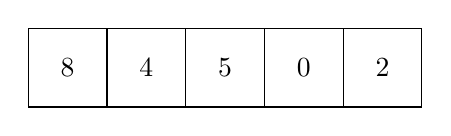
\begin{tikzpicture}
      \draw (0, 0) rectangle (1, 1);
      \node at (0.5, 0.5) {8};
      
      \draw (1, 0) rectangle (2, 1);
      \node at (1.5, 0.5) {4};
      
      \draw (2, 0) rectangle (3, 1);
      \node at (2.5, 0.5) {5};
      
      \draw (3, 0) rectangle (4, 1);
      \node at (3.5, 0.5) {0};
      
      \draw (4, 0) rectangle (5, 1);
      \node at (4.5, 0.5) {2};
  \end{tikzpicture}
\end{center}

\subsection{線形探索の実装}
\begin{lstlisting}[caption=線形探索の実装, frame=TRBL, label={linear}]
def linear_search(array: list[int], value: int) -> int:
    """
    線形探索をして一致するならそのindexを返す. 一致しないときは-1を返す
    """
    for i in range(len(array)):
        if array[i] == value:
            return i
    
    return -1


\end{lstlisting}

\subsection{番兵}

番兵法では探索するデータ集合の最後に目的とする数を追加します。最後に番兵を追加することで、より効率的に探索を行うことができます。
実際には番兵を追加してもそこまで効率が良くなるわけではないですが、番兵を追加することで、ループの条件判定を省略することができます。

\vspace{0.5cm}

\begin{center}
  \begin{tikzpicture}
      \draw (0, 0) rectangle (1, 1);
      \node at (0.5, 0.5) {8};
      
      \draw (1, 0) rectangle (2, 1);
      \node at (1.5, 0.5) {4};
      
      \draw (2, 0) rectangle (3, 1);
      \node at (2.5, 0.5) {5};
      
      \draw (3, 0) rectangle (4, 1);
      \node at (3.5, 0.5) {3};
      
      \draw (4, 0) rectangle (5, 1);
      \node at (4.5, 0.5) {2};
      
      \draw (5, 0) rectangle (6, 1);
      \fill[red, overlay] (5, 0) rectangle (6, 1);
      \node[white] at (5.5, 0.5) {0};
      \node[] at (5.5, -0.5) {番兵};
  \end{tikzpicture}
\end{center}

\begin{lstlisting}[caption=番兵の実装, frame=TRBL, label={sentinel}]
def linear_search(array: list[int], value: int) -> int:
    """
    線形探索をして一致するならそのindexを返す. 一致しないときは-1を返す
    """
    i = 0
    copied_array = array.copy()
    copied_array.append(value)
    while copied_array[i] != value: i += 1
    
    return i if i < len(array) else -1
  \end{lstlisting}

\section{二分探索}

\subsection{配列を探索する二分探索}

二分探索はソートされた配列に対して高速に探索を行うアルゴリズムの一つです。二分探索では探索する区間が条件に応じてどんどん半分になっていくため、
計算量は$O(\log n)$となります。以下の配列に対して、二分探索で18を探す場合を考えましょう。

最初の区間は配列全体を取ります。0-indexedな配列を考えると、midは39となり目的の18より大きいです。midが目的の値より大きい場合、
右の区間を狭めます。right = mid - 1とします。

\vspace{0.5cm}

\begin{center}
  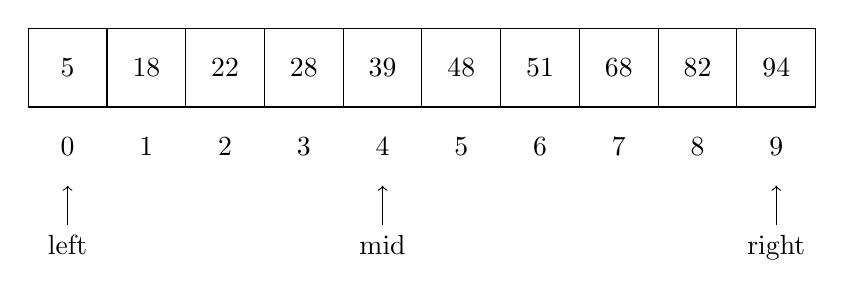
\begin{tikzpicture}
      \draw (0, 0) rectangle (1, 1);
      \node at (0.5, 0.5) {5};
      
      \draw (1, 0) rectangle (2, 1);
      \node at (1.5, 0.5) {18};
      
      \draw (2, 0) rectangle (3, 1);
      \node at (2.5, 0.5) {22};
      
      \draw (3, 0) rectangle (4, 1);
      \node at (3.5, 0.5) {28};
      
      \draw (4, 0) rectangle (5, 1);
      \node at (4.5, 0.5) {39};
      
      \draw (5, 0) rectangle (6, 1);
      \node at (5.5, 0.5) {48};
      
      \draw (6, 0) rectangle (7, 1);
      \node at (6.5, 0.5) {51};
      
      \draw (7, 0) rectangle (8, 1);
      \node at (7.5, 0.5) {68};
      
      \draw (8, 0) rectangle (9, 1);
      \node at (8.5, 0.5) {82};
      
      \draw (9, 0) rectangle (10, 1);
      \node at (9.5, 0.5) {94};

      \foreach \i in {0,1,...,9} {
        \node at (\i+0.5, -0.5) {\i};
    }

      % ラベルをはる
      \draw[<-] (0.5, -1) -- (0.5, -1.5) node[below] {left};
      \draw[<-] (9.5, -1) -- (9.5, -1.5) node[below] {right};
      \draw[<-] (4.5, -1) -- (4.5, -1.5) node[below] {mid};
  \end{tikzpicture}
\end{center}

\vspace{0.5cm}

rightを3に更新しました。mid = (0 + 3) // 2 = 1となります。midの値は18で目的の値と一致します。

\vspace{0.5cm}

\begin{center}
  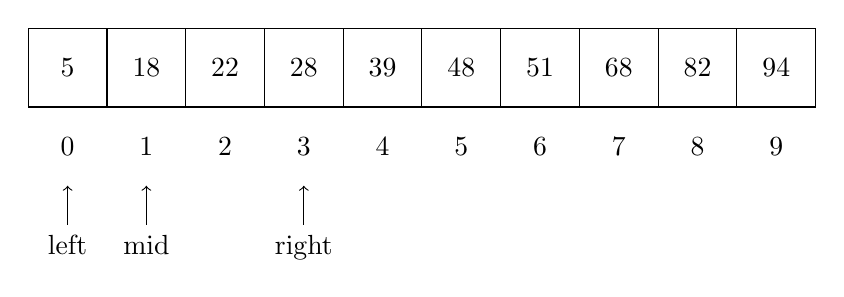
\begin{tikzpicture}
      \draw (0, 0) rectangle (1, 1);
      \node at (0.5, 0.5) {5};
      
      \draw (1, 0) rectangle (2, 1);
      \node at (1.5, 0.5) {18};
      
      \draw (2, 0) rectangle (3, 1);
      \node at (2.5, 0.5) {22};
      
      \draw (3, 0) rectangle (4, 1);
      \node at (3.5, 0.5) {28};
      
      \draw (4, 0) rectangle (5, 1);
      \node at (4.5, 0.5) {39};
      
      \draw (5, 0) rectangle (6, 1);
      \node at (5.5, 0.5) {48};
      
      \draw (6, 0) rectangle (7, 1);
      \node at (6.5, 0.5) {51};
      
      \draw (7, 0) rectangle (8, 1);
      \node at (7.5, 0.5) {68};
      
      \draw (8, 0) rectangle (9, 1);
      \node at (8.5, 0.5) {82};
      
      \draw (9, 0) rectangle (10, 1);
      \node at (9.5, 0.5) {94};

      \foreach \i in {0,1,...,9} {
        \node at (\i+0.5, -0.5) {\i};
    }

      % ラベルをはる
      \draw[<-] (0.5, -1) -- (0.5, -1.5) node[below] {left};
      \draw[<-] (1.5, -1) -- (1.5, -1.5) node[below] {mid};
      \draw[<-] (3.5, -1) -- (3.5, -1.5) node[below] {right};
  \end{tikzpicture}
\end{center}

\vspace{0.5cm}

次に、目的とする値を19として配列に存在しない場合を考えましょう。mid = 1の値は18で目的の値よりも小さいので、下の図のようにleftをmid + 1に更新します。
mid = (2 + 3) // 2 = 2となります。midの値は22で目的の値より大きいです。よって、rightをmid - 1に更新します。
すると、right = 1, left = 2となり、left > rightとなるので探索を終了します。

\vspace{0.5cm}

\begin{center}
  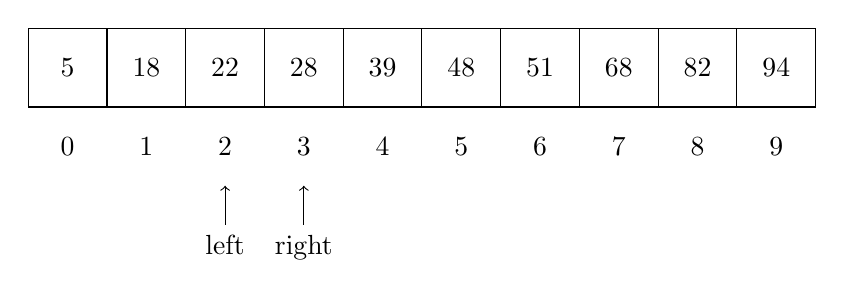
\begin{tikzpicture}
      \draw (0, 0) rectangle (1, 1);
      \node at (0.5, 0.5) {5};
      
      \draw (1, 0) rectangle (2, 1);
      \node at (1.5, 0.5) {18};
      
      \draw (2, 0) rectangle (3, 1);
      \node at (2.5, 0.5) {22};
      
      \draw (3, 0) rectangle (4, 1);
      \node at (3.5, 0.5) {28};
      
      \draw (4, 0) rectangle (5, 1);
      \node at (4.5, 0.5) {39};
      
      \draw (5, 0) rectangle (6, 1);
      \node at (5.5, 0.5) {48};
      
      \draw (6, 0) rectangle (7, 1);
      \node at (6.5, 0.5) {51};
      
      \draw (7, 0) rectangle (8, 1);
      \node at (7.5, 0.5) {68};
      
      \draw (8, 0) rectangle (9, 1);
      \node at (8.5, 0.5) {82};
      
      \draw (9, 0) rectangle (10, 1);
      \node at (9.5, 0.5) {94};

      \foreach \i in {0,1,...,9} {
        \node at (\i+0.5, -0.5) {\i};
    }

      % ラベルをはる
      \draw[<-] (2.5, -1) -- (2.5, -1.5) node[below] {left};
      \draw[<-] (3.5, -1) -- (3.5, -1.5) node[below] {right};
  \end{tikzpicture}
\end{center}

二分探索の実装は以下の通りです。

\begin{lstlisting}[caption=二分探索の実装, frame=TRBL, label={simle_binary}]
def binary_search(A: list[int], value: int) -> int:
    left, right = 0, len(A) - 1
    
    while left <= right:
        mid = (left + right) // 2
        
        if A[mid] == value:
            return mid
        
        if A[mid] < value:
            left = mid + 1
        else:
            right = mid - 1
    
    return -1
\end{lstlisting}

\subsection{一般化した二分探索}
Pythonの標準ライブラリであるbisectのbisect\_leftの実装をしましょう。bisect\_leftはソートされた配列に対して、
与えられた値以上の最小のindexを返す関数です。bisect\_leftは二分探索を用いて実装されています。先ほどの配列から要素を探す二分探索では、要素一致するか否かを判定していましたが、
今回はもっと一般化して「midがある条件を満たすか否か」を判定して範囲を狭めていきます。このとき、leftより右側の区間は
条件を満たさず、rightより左側の区間は条件を満たすようにします。 

二分探索では以下の図のような条件を満たす赤い部分を条件を満たす境界ギリギリになるように更新していきます。

\begin{itemize}
  \item leftは常に条件を満たさない
  \item rightは常に条件を満たす
\end{itemize}

という条件を満たすように処理を進めていき、最終的にleftが条件を満たさない最大のindex、rightが条件を満たす最小のindexを返します。
bisect\_leftではleftが与えられた値よりも小さく、rightが与えられた値以上の最小のindexを返す関数です。

\vspace{0.5cm}

\begin{center}
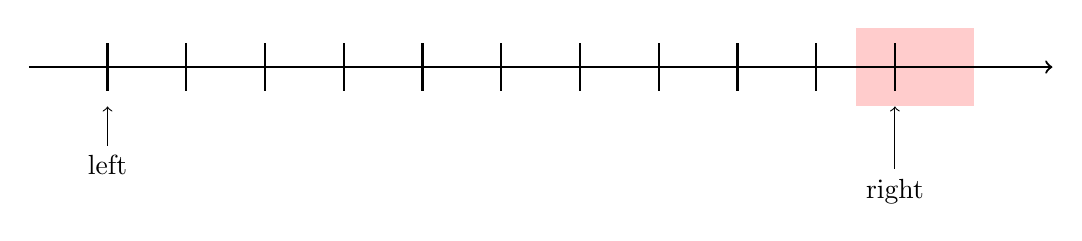
\begin{tikzpicture}
    \fill[red!20] (10.5, 0.5) rectangle (12, 1.5);
    \foreach \x in {1, 2, 3, 4, 5, 6, 7, 8, 9, 10, 11} {
        \draw[thick] (\x, 0.7) -- (\x, 1.3);
    }

    \draw[->, thick] (0, 1) -- (13, 1);
    \draw[<-] (1, 0.5) -- (1, -0.) node[below] {left};
    \draw[<-] (11, 0.5) -- (11, -0.3) node[below] {right};
\end{tikzpicture}
\end{center}

\begin{center}
  \textbf{初期状態}
\end{center}

\vspace{0.5cm}

\begin{center}
  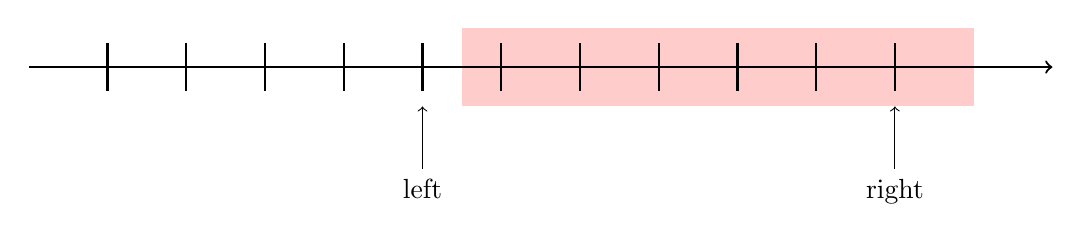
\begin{tikzpicture}
      \fill[red!20] (5.5, 0.5) rectangle (12, 1.5);
      \foreach \x in {1, 2, 3, 4, 5, 6, 7, 8, 9, 10, 11} {
          \draw[thick] (\x, 0.7) -- (\x, 1.3);
      }
  
      \draw[->, thick] (0, 1) -- (13, 1);
      \draw[<-] (5, 0.5) -- (5, -0.3) node[below] {left};
      \draw[<-] (11, 0.5) -- (11, -0.3) node[below] {right};
  \end{tikzpicture}
  \end{center}
  
  \begin{center}
    \textbf{終了状態}
  \end{center}

bisect\_leftの実装は以下の通りです。

\begin{lstlisting}[caption=bisect\_leftの実装, frame=TRBL, label={bisect_left}]
def bisect_left(array: list[int], key: int) -> int:
  left, right = -1, len(array)
  
  while right - left > 1:
      mid = (left + right) // 2
      
      if array[mid] < key:
          left = mid
      else:
          right = mid
  
  return right
\end{lstlisting}

bisect\_leftの実装では、左側が条件を満たさない、右側が条件を満たすといった実装になっています。これだとまだ条件次第でleftが条件を満たす、rightが条件を満たさないという
実装もあり得ます。そこで以下ではめぐる式二分探索のさらに一般化した実装を紹介します。

\subsection{めぐる式二分探索}

めぐる式二分探索では、

\begin{itemize}
  \item ngは常に条件を満たさない
  \item okは常に条件を満たす
\end{itemize}

のように数直線上の右や左という概念を持たせずに実装します。めぐる式二分探索は以下のように実装されます。
is\_okは条件を満たすかどうかを判定する関数ですので、条件に合わせて実装します。

\begin{lstlisting}[caption=めぐる式二分探索, frame=TRBL, label={megru}]
def binary_search(array: list[int], key: int):
    ng, ok = -1, len(array)
    
    while abs(ok - ng) > 1:
        mid = (ng + ok) // 2
        
        if is_ok(array, mid, key):
            ok = mid
        else:
            ng = mid
    
    return ok
\end{lstlisting}

\newpage

\section{二分探索木}
二分探索は探索自体は$O(\log n)$で行うことができますが、配列がソートされているひつようがあり、データの挿入や削除がある場合は毎回ソートがあり非効率ではあります。
解決策としては、\textbf{データ構造で解決}や\textbf{Treeq}などがあります。データ構造で解決する方法の一つが\textbf{二分探索木}です。

\textbf{二分探索木}は以下の性質を持った木構造です。

\begin{itemize}
  \item 左子ノードは親ノードよりも小さい(または等しい) (下の図では$B \leq A$)
  \item 右子ノードは親ノードよりも大きい (下の図では$A < C$)
\end{itemize}

\begin{center}
    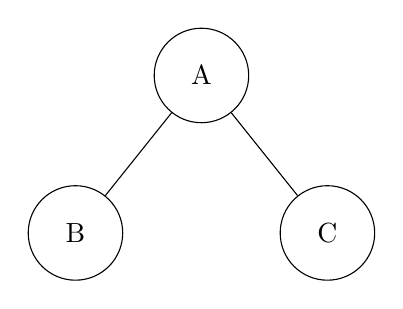
\begin{tikzpicture}[scale=0.4]
      \node[circle, draw, minimum size=1.2cm] (A) at (0, 0) {};
      \node[circle, draw, minimum size=1.2cm] (B) at (-4, -5) {};
      \node[circle, draw, minimum size=1.2cm] (C) at (4, -5) {};

      % 線を引く
      \draw (A) --(B);
      \draw (A) -- (C);

      % 値を入れる
      \node at (0, 0) {A};
      \node at (-4, -5) {B};
      \node at (4, -5) {C};
    \end{tikzpicture}
\end{center}

二分探索木で行う処理は以下の通りです。

\begin{itemize}
  \item 木の作成
  \item 探索
  \item 削除
\end{itemize}

\subsection{二分探索木の作成}
\texttt{[22,18, 5, 82, 51, 39]}の配列を二分探索木に変換してみましょう。

\vspace{0.5cm}

\begin{center}
  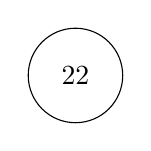
\begin{tikzpicture}
    \node[circle, draw, minimum size=1.2cm] (A) at (0, 0) {}; 

    % 値を入れる
    \node at (0, 0) {22};
  \end{tikzpicture}
\end{center}

\begin{center}
  \textbf{22を挿入}
\end{center}

\vspace{0.5cm}

\begin{center}
  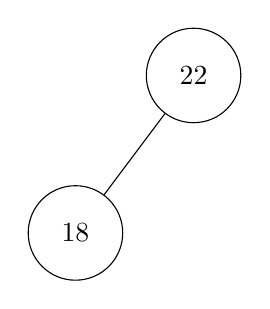
\begin{tikzpicture}
    \node[circle, draw, minimum size=1.2cm] (A) at (0, 0) {}; 
    \node[circle, draw, minimum size=1.2cm] (B) at (-1.5, -2) {};

    % 線を引く
    \draw (A) --(B);

    % 値を入れる
    \node at (0, 0) {22};
    \node at (-1.5, -2) {18};
  \end{tikzpicture}
\end{center}

\begin{center}
  \textbf{18を挿入}
\end{center}

\vspace{0.5cm}

\begin{center}
  \begin{tikzpicture}
    \node[circle, draw, minimum size=1.2cm] (A) at (0, 0) {}; 
    \node[circle, draw, minimum size=1.2cm] (B) at (-1.5, -2) {};
    \node[circle, draw, minimum size=1.2cm] (C) at (-3, -4) {};

    % 線を引く
    \draw (A) --(B);
    \draw (B) -- (C);

    % 値を入れる
    \node at (0, 0) {22};
    \node at (-1.5, -2) {18};
    \node at (-3, -4) {5};
  \end{tikzpicture}
\end{center}

\begin{center}
  \textbf{5を挿入}
\end{center}

\vspace{0.5cm}

\begin{center}
  \begin{tikzpicture}
    \node[circle, draw, minimum size=1.2cm] (A) at (0, 0) {}; 
    \node[circle, draw, minimum size=1.2cm] (B) at (-1.5, -2) {};
    \node[circle, draw, minimum size=1.2cm] (C) at (-3, -4) {};
    \node[circle, draw, minimum size=1.2cm] (D) at (1.5, -2) {};

    % 線を引く
    \draw (A) --(B);
    \draw (B) -- (C);
    \draw (A) -- (D);

    % 値を入れる
    \node at (0, 0) {22};
    \node at (-1.5, -2) {18};
    \node at (-3, -4) {5};
    \node at (1.5, -2) {82};
  \end{tikzpicture}
\end{center}

\begin{center}
  \textbf{82を挿入}
\end{center}

\vspace{0.5cm}

\begin{center}
  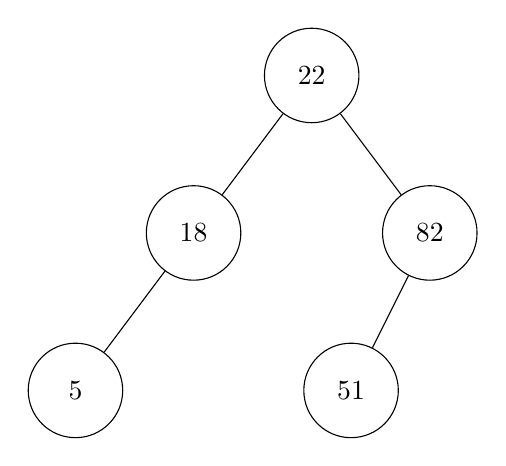
\begin{tikzpicture}
    \node[circle, draw, minimum size=1.2cm] (A) at (0, 0) {}; 
    \node[circle, draw, minimum size=1.2cm] (B) at (-1.5, -2) {};
    \node[circle, draw, minimum size=1.2cm] (C) at (-3, -4) {};
    \node[circle, draw, minimum size=1.2cm] (D) at (1.5, -2) {};
    \node[circle, draw, minimum size=1.2cm] (E) at (0.5, -4) {};

    % 線を引く
    \draw (A) --(B);
    \draw (B) -- (C);
    \draw (A) -- (D);
    \draw (D) -- (E);

    % 値を入れる
    \node at (0, 0) {22};
    \node at (-1.5, -2) {18};
    \node at (-3, -4) {5};
    \node at (1.5, -2) {82};
    \node at (0.5, -4) {51};
  \end{tikzpicture}
\end{center}

\begin{center}
  \textbf{51を挿入}
\end{center}

\vspace{0.5cm}

\begin{center}
  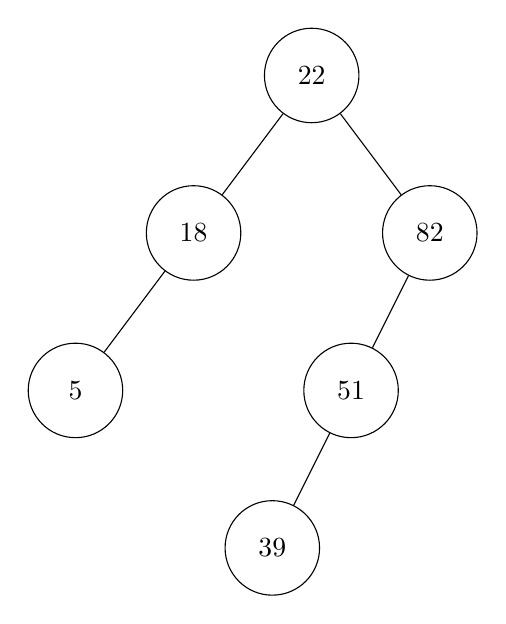
\begin{tikzpicture}
    \node[circle, draw, minimum size=1.2cm] (A) at (0, 0) {}; 
    \node[circle, draw, minimum size=1.2cm] (B) at (-1.5, -2) {};
    \node[circle, draw, minimum size=1.2cm] (C) at (-3, -4) {};
    \node[circle, draw, minimum size=1.2cm] (D) at (1.5, -2) {};
    \node[circle, draw, minimum size=1.2cm] (E) at (0.5, -4) {};
    \node[circle, draw, minimum size=1.2cm] (F) at (-0.5, -6) {};

    % 線を引く
    \draw (A) --(B);
    \draw (B) -- (C);
    \draw (A) -- (D);
    \draw (D) -- (E);
    \draw (E) -- (F);

    % 値を入れる
    \node at (0, 0) {22};
    \node at (-1.5, -2) {18};
    \node at (-3, -4) {5};
    \node at (1.5, -2) {82};
    \node at (0.5, -4) {51}; 
    \node at (-0.5, -6) {39};

  \end{tikzpicture}
\end{center}

\begin{center}
  \textbf{39を挿入}
\end{center}

\subsection{二分探索木の探索}
上の木を例に51を探してみましょう。根から順に探していきます。
\vspace{0.5cm}

\begin{center}
  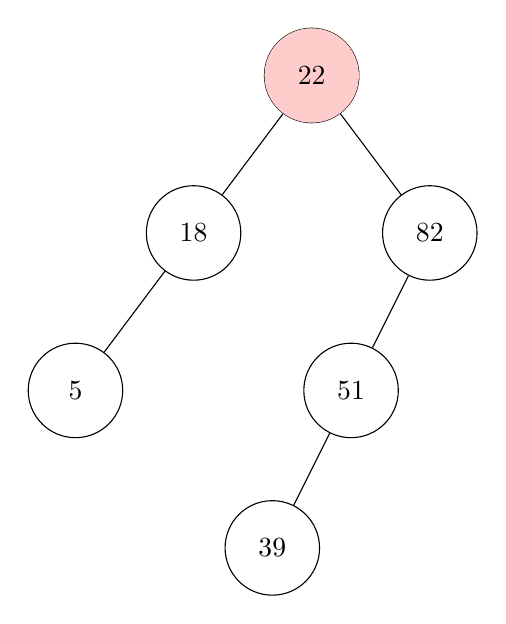
\begin{tikzpicture}
    \node[circle, draw, minimum size=1.2cm] (A) at (0, 0) {}; 
    \node[circle, draw, minimum size=1.2cm] (B) at (-1.5, -2) {};
    \node[circle, draw, minimum size=1.2cm] (C) at (-3, -4) {};
    \node[circle, draw, minimum size=1.2cm] (D) at (1.5, -2) {};
    \node[circle, draw, minimum size=1.2cm] (E) at (0.5, -4) {};
    \node[circle, draw, minimum size=1.2cm] (F) at (-0.5, -6) {};

    % 色を塗る
    \fill[red!20] (0, 0) circle (0.6);

    % 線を引く
    \draw (A) --(B);
    \draw (B) -- (C);
    \draw (A) -- (D);
    \draw (D) -- (E);
    \draw (E) -- (F);

    % 値を入れる
    \node at (0, 0) {22};
    \node at (-1.5, -2) {18};
    \node at (-3, -4) {5};
    \node at (1.5, -2) {82};
    \node at (0.5, -4) {51}; 
    \node at (-0.5, -6) {39};

  \end{tikzpicture}
\end{center}

\vspace{0.5cm}

51は22よりも大きいので右の子ノードに進みます。

\begin{center}
  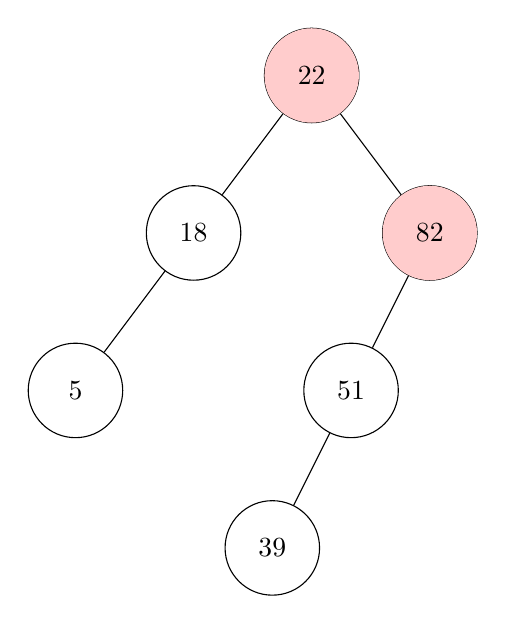
\begin{tikzpicture}
    \node[circle, draw, minimum size=1.2cm] (A) at (0, 0) {}; 
    \node[circle, draw, minimum size=1.2cm] (B) at (-1.5, -2) {};
    \node[circle, draw, minimum size=1.2cm] (C) at (-3, -4) {};
    \node[circle, draw, minimum size=1.2cm] (D) at (1.5, -2) {};
    \node[circle, draw, minimum size=1.2cm] (E) at (0.5, -4) {};
    \node[circle, draw, minimum size=1.2cm] (F) at (-0.5, -6) {};

    % 色を塗る
    \fill[red!20] (0, 0) circle (0.6);
    \fill[red!20] (1.5, -2) circle (0.6);

    % 線を引く
    \draw (A) --(B);
    \draw (B) -- (C);
    \draw (A) -- (D);
    \draw (D) -- (E);
    \draw (E) -- (F);

    % 値を入れる
    \node at (0, 0) {22};
    \node at (-1.5, -2) {18};
    \node at (-3, -4) {5};
    \node at (1.5, -2) {82};
    \node at (0.5, -4) {51}; 
    \node at (-0.5, -6) {39};

  \end{tikzpicture}
\end{center}

51は82よりも小さいので左の子ノードに進みます。見つかりました。

\vspace{0.5cm}

\begin{center}
  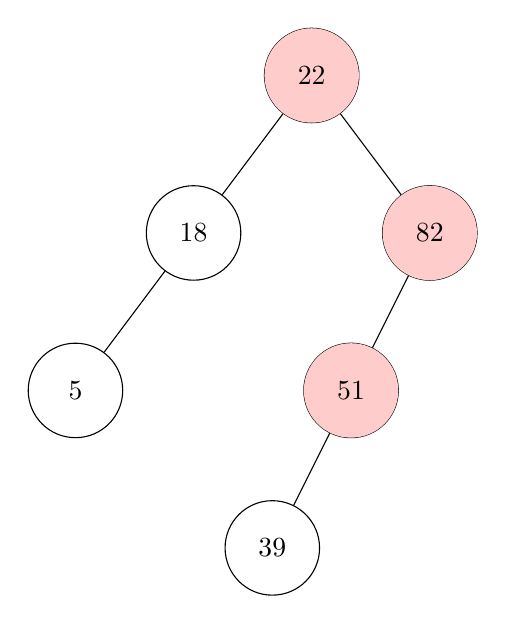
\begin{tikzpicture}
    \node[circle, draw, minimum size=1.2cm] (A) at (0, 0) {}; 
    \node[circle, draw, minimum size=1.2cm] (B) at (-1.5, -2) {};
    \node[circle, draw, minimum size=1.2cm] (C) at (-3, -4) {};
    \node[circle, draw, minimum size=1.2cm] (D) at (1.5, -2) {};
    \node[circle, draw, minimum size=1.2cm] (E) at (0.5, -4) {};
    \node[circle, draw, minimum size=1.2cm] (F) at (-0.5, -6) {};

    % 色を塗る
    \fill[red!20] (0, 0) circle (0.6);
    \fill[red!20] (1.5, -2) circle (0.6);
    \fill[red!20] (0.5, -4) circle (0.6);

    % 線を引く
    \draw (A) --(B);
    \draw (B) -- (C);
    \draw (A) -- (D);
    \draw (D) -- (E);
    \draw (E) -- (F);

    % 値を入れる
    \node at (0, 0) {22};
    \node at (-1.5, -2) {18};
    \node at (-3, -4) {5};
    \node at (1.5, -2) {82};
    \node at (0.5, -4) {51}; 
    \node at (-0.5, -6) {39};

  \end{tikzpicture}
\end{center}

\subsection{二分探索木の削除}

二分探索木からノードを削除する場合は以下の3つのケースがあります。

\begin{itemize}
  \item 子ノードがない場合
  \item 子ノードが1つの場合
  \item 子ノードが2つの場合
\end{itemize}

\subsubsection{子ノードがない場合}
例えば5を削除する場合を考えます。5は左右の子ノードがないので、他のノードに影響がないためそのまま削除します。

\begin{center}
  \begin{tikzpicture}
    \node[circle, draw, minimum size=1.2cm] (A) at (0, 0) {}; 
    \node[circle, draw, minimum size=1.2cm] (B) at (-1.5, -2) {};
    \node[circle, draw, minimum size=1.2cm, dotted] (C) at (-3, -4) {};
    \node[circle, draw, minimum size=1.2cm] (D) at (1.5, -2) {};
    \node[circle, draw, minimum size=1.2cm] (E) at (0.5, -4) {};
    \node[circle, draw, minimum size=1.2cm] (F) at (-0.5, -6) {};

    % 線を引く
    \draw (A) --(B);
    \draw [dotted] (B) -- (C);
    \draw (A) -- (D);
    \draw (D) -- (E);
    \draw (E) -- (F);

    % 値を入れる
    \node at (0, 0) {22};
    \node at (-1.5, -2) {18};
    \node at (-3, -4) {5};
    \node at (1.5, -2) {82};
    \node at (0.5, -4) {51}; 
    \node at (-0.5, -6) {39};

  \end{tikzpicture}
\end{center}

\subsubsection{子ノードが1つの場合}
次に18を削除する場合を考えます。18は左の子ノードが5しか持っていないので、5を18の位置に移動させます。18は親ノードから見て
左の子ノードですが、右ノードの場合も同様に処理します。

\vspace{0.5cm}

\begin{center}
  \begin{tikzpicture}
    \node[circle, draw, minimum size=1.2cm] (A) at (0, 0) {}; 
    \node[circle, draw, minimum size=1.2cm] (B) at (-1.5, -2) {};
    \node[circle, draw, minimum size=1.2cm, dotted] (C) at (-3, -4) {};
    \node[circle, draw, minimum size=1.2cm] (D) at (1.5, -2) {};
    \node[circle, draw, minimum size=1.2cm] (E) at (0.5, -4) {};
    \node[circle, draw, minimum size=1.2cm] (F) at (-0.5, -6) {};

    % 線を引く
    \draw (A) --(B);
    \draw [dotted] (B) -- (C);
    \draw (A) -- (D);
    \draw (D) -- (E);
    \draw (E) -- (F);

    % 値を入れる
    \node at (0, 0) {22};
    \node at (-1.5, -2) {5};
    \node at (-3, -4) {};
    \node at (1.5, -2) {82};
    \node at (0.5, -4) {51}; 
    \node at (-0.5, -6) {39};

  \end{tikzpicture}
\end{center}

\subsubsection{子ノードが2つの場合}
最後に22を削除する場合を考えます。削除するノードが2つの子ノードを持っている場合は、削除するノードの左の子ノードの最大値か、右の子ノードの最小値を持ってきて、
削除するノードに移動させます。ここでは、22の右の子ノードの最小値39を持ってきて、22の位置に移動させます。

\vspace{0.5cm}

\begin{center}
  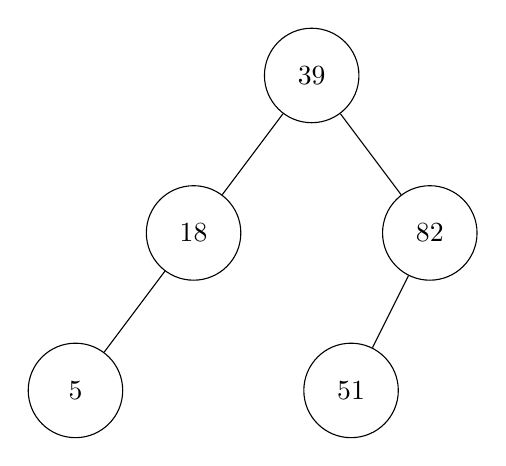
\begin{tikzpicture}
    \node[circle, draw, minimum size=1.2cm] (A) at (0, 0) {}; 
    \node[circle, draw, minimum size=1.2cm] (B) at (-1.5, -2) {};
    \node[circle, draw, minimum size=1.2cm] (C) at (-3, -4) {};
    \node[circle, draw, minimum size=1.2cm] (D) at (1.5, -2) {};
    \node[circle, draw, minimum size=1.2cm] (E) at (0.5, -4) {};

    % 線を引く
    \draw (A) --(B);
    \draw (B) -- (C);
    \draw (A) -- (D);
    \draw (D) -- (E);

    % 値を入れる
    \node at (0, 0) {39};
    \node at (-1.5, -2) {18};
    \node at (-3, -4) {5};
    \node at (1.5, -2) {82};
    \node at (0.5, -4) {51}; 

  \end{tikzpicture}
\end{center}

\subsection{二分木の実装}
\begin{lstlisting}[caption=二分木の実装, frame=TRBL, label={binary_tree}]
class Node:
  def __init__(self, data: int) -> None:
      self.data: int = data
      self.right: Node | None = None
      self.left: Node | None = None
      
  def __str__(self) -> str:
      return str(self.data)
  
class BinarySearchTree:
  def __init__(self):
      self.root = None
      
  def create(self, array: list[int]) -> None:
      for i in range(len(array)):
          self.insert(array[i])
  
  def insert(self, data: int) -> None:
      if self.root is None:
          self.root = Node(data)
      else:
          self._insert_recursively(self.root, data)
  
  def _insert_recursively(self, node: Node, data: int) -> None:
      if data <= node.data:
          if node.left is None:
              node.left = Node(data)
          else:
              self._insert_recursively(node.left, data)
      else:
          if node.right is None:
              node.right = Node(data)
          else:
              self._insert_recursively(node.right, data)
  
  def search(self, value: int) -> Node | None:
      if self.root is None:
          return self.root
      
      return self._search_recursively(self.root, value)
      
  def _search_recursively(self, node: Node, value: int) -> Node | None:
      if node.data == value:
          return node
      
      if value < node.data:
          if node.left is None:
              return node.left
          else:
              return self._search_recursively(node.left, value)
      else:
          if node.right is None:
              return node.right
          else:
              return self._search_recursively(node.right, value)
  
  def delete(self, value: int) -> Node | None:
      if self.root is None:
          return self.root
      else:
          self.root = self._delete_recursively(self.root, value)
  
  def _delete_recursively(self, node: Node, value: int) -> Node | None:
      if value < node.data:
          if node.left is None:
              return None
          else:
              node.left = self._delete_recursively(node.left, value)
      elif value > node.data:
          if node.right is None:
              return None
          else:
              node.right = self._delete_recursively(node.right, value)
      else:
          if node.left is None and node.right is None:
              return None
          elif node.left is None:
              return node.right
          elif node.right is None:
              return node.left
          else:
              successor = self._successor()
              node.data = successor.data
              self._delete_recursively(node.right, successor.data)
              
      return node
  
  def _successor(self) -> Node | None:
      if self.root is None:
          return self.root
      
      node = self.root
      
      while node.left is not None:
          node = node.left
      
      return node
\end{lstlisting}

\newpage

\section{平衡木}
\subsection{二分木の問題点}
二分木は最悪の場合木が以下のように片方に伸びてしまった場合、計算量が$O(n)$になってしまいます。

\vspace{0.5cm}

\begin{center}
  \begin{tikzpicture}[scale=0.6]
    \node[circle, draw, minimum size=1.2cm] (A) at (0, 0) {}; 
    \node[circle, draw, minimum size=1.2cm] (B) at (1.5, -2) {};
    \node[circle, draw, minimum size=1.2cm] (C) at (3, -4) {};
    \node[circle, draw, minimum size=1.2cm] (D) at (4.5, -6) {};
    \node[circle, draw, minimum size=1.2cm] (E) at (6, -8) {};

    % 線を引く
    \draw (A) --(B);
    \draw (B) -- (C);
    \draw (C) -- (D);
    \draw (D) -- (E);

    % 値を入れる
    \node at (0, 0) {1};
    \node at (1.5, -2) {2};
    \node at (3, -4) {3};
    \node at (4.5, -6) {4};
    \node at (6, -8) {5};

  \end{tikzpicture}
\end{center}

\vspace{0.5cm}

\subsection{平衡木}
平衡木は\textbf{回転}や乱択アルゴリズムを用いて木の高さを自動的に小さくする方向に調整できる木構造です。

扱う平衡木の代表的なものには以下のものがあります。

\begin{itemize}
  \item AVL木
  \item 赤黒木
  \item B木
  \item Treap
\end{itemize}

\subsection{AVL木}
AVL木とは、\textbf{Adelson-Velsky and Landis}の名前から取られた木構造で、以下の性質を持ちます。

\begin{itemize}
  \item 任意のノードにおいて、左右の部分木の高さの差が1以下である
\end{itemize}

\vspace{0.5cm}

以降の考察のために\textbf{balance factor}という言葉を導入します。

\begin{definitionbox}[balance factor]
  あるノードの左部分木の高さから右部分木の高さを引いた値を\textbf{balance factor}といいます。
  \begin{itemize}
    \item balance factor = 左部分木の高さ - 右部分木の高さ
  \end{itemize}
\end{definitionbox}

AVL木の性質をbalance factorを使って表すと以下のようになります。

\begin{itemize}
  \item 任意のノードにおいて、balance factorは-1, 0, 1のいずれかである
\end{itemize}

AVL木の例を以下に示します。ノードの横に書いてあるのがbalance factorです。

\vspace{0.5cm}

\begin{center}
  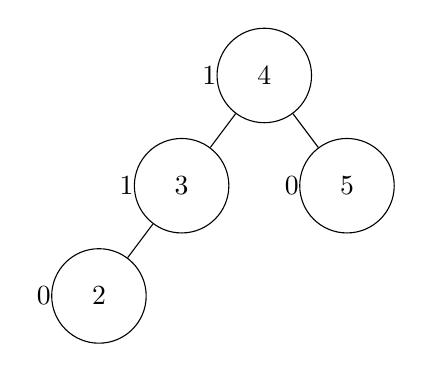
\begin{tikzpicture}[scale=0.7]
    \node[circle, draw, minimum size=1.2cm] (A) at (0, 0) {4}; 
    \node[circle, draw, minimum size=1.2cm] (B) at (-1.5, -2) {3};
    \node[circle, draw, minimum size=1.2cm] (C) at (-3, -4) {2};
    \node[circle, draw, minimum size=1.2cm] (E) at (1.5, -2) {5};


    % 線を引く
    \draw (A) --(B);
    \draw (B) -- (C);
    \draw (A) -- (E);

    % balance factor
    \node at (0 - 1, -1 + 1) {1};
    \node at (-1.5 - 1, -3 + 1) {1};
    \node at (-3 - 1, -5 + 1) {0};
    \node at (1.5 - 1, -3 + 1) {0};

  \end{tikzpicture}
\end{center}

次はAVL木の条件を満たしていない木です。
\vspace{0.5cm}

\begin{center}
  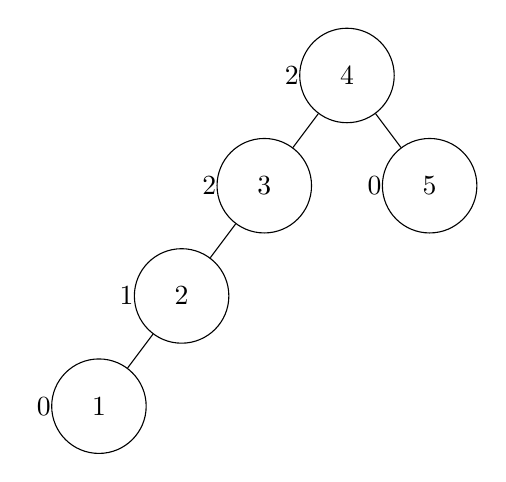
\begin{tikzpicture}[scale=0.7]
    \node[circle, draw, minimum size=1.2cm] (A) at (0, 0) {4}; 
    \node[circle, draw, minimum size=1.2cm] (B) at (-1.5, -2) {3};
    \node[circle, draw, minimum size=1.2cm] (C) at (-3, -4) {2};
    \node[circle, draw, minimum size=1.2cm] (D) at (-4.5, -6) {1};
    \node[circle, draw, minimum size=1.2cm] (E) at (1.5, -2) {5};


    % 線を引く
    \draw (A) --(B);
    \draw (B) -- (C);
    \draw (C) -- (D);
    \draw (A) -- (E);

    % balance factor
    \node at (0 - 1, -1 + 1) {2};
    \node at (-1.5 - 1, -3 + 1) {2};
    \node at (-3 - 1, -5 + 1) {1};
    \node at (-4.5 - 1, -7 + 1) {0};
    \node at (1.5 - 1, -3 + 1) {0};

  \end{tikzpicture}
\end{center}

\newpage

1. 左回転
\begin{center}
\begin{tikzpicture}[scale=0.7, every node/.style={circle, draw, minimum size=1.2cm}]
  \node (A) at (0, 2) {A}; 
  \node (B) at (2, 0) {B};
  \node (C) at (4, -2) {C};

  \draw (A) -- (B);
  \draw (B) -- (C);

  \node[draw=none, fill=none] at (7, 1) {$\longrightarrow$};
  \node[draw=none, fill=none] at (7, 2.5) {左回転};
  
  \node (B1) at (12, 2) {B}; 
  \node (A1) at (10, 0) {A};
  \node (C1) at (14, 0) {C};

  \draw (B1) -- (A1);
  \draw (B1) -- (C1);

  % balance factor
  \node[draw=none, fill=none] at (0, 2 + 1 + 0.2) {-2};
  \node[draw=none, fill=none] at (2, 0 + 1 + 0.2) {-1};
  \node[draw=none, fill=none] at (4, -2 + 1 + 0.2) {0};

  \node[draw=none, fill=none] at (12, 2 + 1 + 0.2) {0};
  \node[draw=none, fill=none] at (10, 0 + 1 + 0.2) {0};
  \node[draw=none, fill=none] at (14, 0 + 1 + 0.2) {0};
\end{tikzpicture}
\end{center}

2. 右回転
\begin{center}
  \begin{tikzpicture}[scale=0.7, every node/.style={circle, draw, minimum size=1.2cm}]    
    \node[draw=none, fill=none] at (6, 1) {$\longrightarrow$};
    \node[draw=none, fill=none] at (6, 2.5) {右回転};
    
    \node (C2) at (2, 2) {A}; 
    \node (B2) at (0, 0) {B};
    \node (A2) at (-2, -2) {C};
  
    \draw (C2) -- (B2);
    \draw (B2) -- (A2);
  
    \node (B3) at (12, 2) {B}; 
    \node (C3) at (10, 0) {C};
    \node (A3) at (14, 0) {A};

    \draw (B3) -- (C3);
    \draw (B3) -- (A3);

    % balance factor
    \node[draw=none, fill=none] at (2, 2 + 1 + 0.2) {2};
    \node[draw=none, fill=none] at (0, 0 + 1 + 0.2) {1};
    \node[draw=none, fill=none] at (-2, -2 + 1 + 0.2) {0};

    \node[draw=none, fill=none] at (12, 2 + 1 + 0.2) {0};
    \node[draw=none, fill=none] at (10, 0 + 1 + 0.2) {0};
    \node[draw=none, fill=none] at (14, 0 + 1 + 0.2) {0};
  \end{tikzpicture}
\end{center}

\vspace{0.5cm}

3. 左右回転
\begin{center}
  \begin{tikzpicture}[scale=0.7, every node/.style={circle, draw, minimum size=1.2cm}]    
    % 1個目の木 (Original Tree)
    \node (A) at (0, 2) {A}; 
    \node (C) at (-2, 0) {B};
    \node (B) at (0, -2) {C};

    \draw (A) -- (C);
    \draw (C) -- (B);

    % Arrow for Left Rotation
    \node[draw=none, fill=none] at (4, 1) {$\longrightarrow$};
    \node[draw=none, fill=none] at (4, 2.5) {左回転};
    
    % 2個目の木 (Intermediate Tree after Left Rotation)
    \node (A1) at (8, 2) {A}; 
    \node (B1) at (6, 0) {B};
    \node (C1) at (4, -2) {C};

    \draw (A1) -- (B1);
    \draw (B1) -- (C1);

    % Arrow for Right Rotation
    \node[draw=none, fill=none] at (12, 1) {$\longrightarrow$};
    \node[draw=none, fill=none] at (12, 2.5) {右回転};
    
    % 3個目の木 (Final Balanced Tree after Right Rotation)
    \node (B2) at (16, 2) {A}; 
    \node (A2) at (14, 0) {B};
    \node (C2) at (18, 0) {C};

    % Drawing the edges
    \draw (B2) -- (A2);
    \draw (B2) -- (C2);

    % balance factor
    \node[draw=none, fill=none] at (0, 2 + 1 + 0.2) {2};
    \node[draw=none, fill=none] at (-2, 0 + 1 + 0.2) {-1};
    \node[draw=none, fill=none] at (0, -2 + 1 + 0.2) {0};

    \node[draw=none, fill=none] at (8, 2 + 1 + 0.2) {2};
    \node[draw=none, fill=none] at (6, 0 + 1 + 0.2) {1};
    \node[draw=none, fill=none] at (4, -2 + 1 + 0.2) {0};

    \node[draw=none, fill=none] at (16, 2 + 1 + 0.2) {0};
    \node[draw=none, fill=none] at (14, 0 + 1 + 0.2) {0};
    \node[draw=none, fill=none] at (18, 0 + 1 + 0.2) {0};
  \end{tikzpicture}
\end{center}

4. 右左回転

\begin{center}
  \begin{tikzpicture}[scale=0.7, every node/.style={circle, draw, minimum size=1.2cm}]    
    % 1個目の木 (Original Tree)
    \node (A) at (0, 2) {A}; 
    \node (B) at (2, 0) {B};
    \node (C) at (0, -2) {C};

    \draw (A) -- (B);
    \draw (B) -- (C);

    % Arrow for Right Rotation
    \node[draw=none, fill=none] at (6, 1) {$\longrightarrow$};
    \node[draw=none, fill=none] at (6, 2.5) {右回転};
    
    % 2個目の木 (Intermediate Tree after Right Rotation)
    \node (B1) at (10, 2) {B}; 
    \node (A1) at (12, 0) {A};
    \node (C1) at (14, -2) {C};

    \draw (B1) -- (A1);
    \draw (A1) -- (C1);

    % Arrow for Left Rotation
    \node[draw=none, fill=none] at (16, 1) {$\longrightarrow$};
    \node[draw=none, fill=none] at (16, 2.5) {左回転};
    
    % 3個目の木 (Final Balanced Tree after Left Rotation)
    \node (B2) at (20, 2) {B}; 
    \node (A2) at (18, 0) {A};
    \node (C2) at (22, 0) {C};

    % Drawing the edges
    \draw (B2) -- (A2);
    \draw (B2) -- (C2);

    % balance factor
    \node[draw=none, fill=none] at (0, 2 + 1 + 0.2) {-2};
    \node[draw=none, fill=none] at (2, 0 + 1 + 0.2) {1};
    \node[draw=none, fill=none] at (0, -2 + 1 + 0.2) {0};

    \node[draw=none, fill=none] at (10, 2 + 1 + 0.2) {-2};
    \node[draw=none, fill=none] at (12, 0 + 1 + 0.2) {-1};
    \node[draw=none, fill=none] at (14, -2 + 1 + 0.2) {0};

    \node[draw=none, fill=none] at (20, 2 + 1 + 0.2) {0};
    \node[draw=none, fill=none] at (18, 0 + 1 + 0.2) {0};
    \node[draw=none, fill=none] at (22, 0 + 1 + 0.2) {0};
  \end{tikzpicture}
\end{center}

  \begin{lstlisting}[caption=二分ヒープの実装, label=binaryheap, frame=TRBL, label={binaryheap}]
  class Node:
      def \_\_init\_\_(self, value: int) -> None:
          self.data: int = value
          self.left: Node | None = None
          self.right: Node | None = None
          self.height: int = 0
      
      def \_\_str\_\_(self) -> str:
          return f"Node: data = {self.data} height = {self.height}"
          
  class AVLTree:
      def \_\_init\_\_(self):
          self.root = None
      
      def \_height(self, node: Node | None) -> int:
          if node is None:
              return -1
          
          return node.height
          
      def \_update\_height(self, node:
       Node) -> None:
          node.height = 1 + max(self.\_height(node.left), self.\_height(node.right))
  
      def \_balance\_factor(self, node: Node) -> int:
          return self.\_height(node.left) - self.\_height(node.right)
  
      def \_right\_rotate(self, node: Node) -> Node:
          new\_root = node.left
          node.left = new\_root.right
          new\_root.right = node
          
          self.\_update\_height(node)
          self.\_update\_height(new\_root)
          
          return new\_root 
      
      def \_left\_rotate(self, node: Node) -> Node:
          new\_root = node.right
          node.right = new\_root.left
          new\_root.left = node
          
          self.\_update\_height(node)
          self.\_update\_height(new\_root)
          
          return new\_root
          
      def create(self, values: list[int]) -> None:
          for value in values:
              self.insert(value)
      
      def insert(self, value: int) -> None:
          if self.root is None:
              self.root = Node(value)
              return self.root
          else:
              self.root = self.\_insert\_recursively(self.root, value)
              return self.root
      
      def \_insert\_recursively(self, node: Node, value: int) -> Node:
          if value <= node.data:
              if node.left is None:
                  node.left = Node(value)
              else:
                  node.left = self.\_insert\_recursively(node.left, value)
          else:
              if node.right is None:
                  node.right = Node(value)
              else:
                  node.right = self.\_insert\_recursively(node.right, value)
          
          self.\_update\_height(node)
          
          balance\_factor = self.\_balance\_factor(node)
          
          if balance\_factor > 1 and value < node.left.data:
              return self.\_right\_rotate(node)
          
          if balance\_factor > 1 and value > node.left.data:
              node.left = self.\_left\_rotate(node.left)
              return self.\_right\_rotate(node)
          
          if balance\_factor < -1 and value > node.right.data:
              return self.\_left\_rotate(node)
          
          if balance\_factor < -1 and value < node.right.data:
              node.right = self.\_right\_rotate(node.right)
              return self.\_left\_rotate(node)
          
          return node
          
      
      def search(self, value: int) -> Node | None:
          if self.root is None:
              return None
          
          return self.\_search\_recursively(self.root, value)
  
      def \_search\_recursively(self, node: Node, value: int) -> Node | None:
          if value == node.data:
              return node
          
          if value < node.data:
              if node.left is None:
                  return None
              else:
                  return self.\_search\_recursively(node.left, value)
          else:
              if node.right is None:
                  return None
              else:
                  return self.\_search\_recursively(node.right, value)
              
      
      def delete(self, value: int) -> Node | None:
          if self.root is None:
              return self.root
          else:
              self.root = self.\_delete\_recursively(self.root, value)
              return self.root
      
      def \_delete\_recursively(self, node: Node, value: int) -> Node | None:
          if value < node.data:
              node.left = self.\_delete\_recursively(node.left, value)
          elif value > node.data:
              node.right = self.\_delete\_recursively(node.right, value)
          else:
              if node.left is None and node.right is None:
                  return None
              elif node.left is None:
                  return node.right
              elif node.right is None:
                  return node.left
              else:
                  min\_node = self.\_find\_min(node.right)
                  node.data = min\_node.data
                  node.right = self.\_delete\_recursively(node.right, min\_node.data)
          
          self\.\_update\_height(node)
          
          balance\_factor = self.\_balance\_factor(node)
          
          if balance\_factor > 1 and self.\_balance\_factor(node.left) >= 0:
              return self.\_right\_rotate(node)
          
          if balance\_factor < -1 and self.\_balance\_factor(node.right) <= 0:
              return self.\_left\_rotate(node)
          
          if balance\_factor > 1 and self.\_balance\_factor(node.left) < 0:
              node.left = self.\_left\_rotate(node.left)
              return self.\_right\_rotate(node)
          
          if balance\_factor < -1 and self.\_balance\_factor(node.right) > 0:
              node.right = self.\_right\_rotate(node.right)
              return self.\_left\_rotate(node)
          
          return node
  \end{lstlisting}

\newpage
\subsection{B木}
AVL木は二分木であるため、データの数が多い場合に気が高くなり検索や挿入に時間がかかってしまう問題があります。そこで枝の数が
2本よりも多く取るB木というデータ構造を紹介します。B木は応用範囲が広く以下の様な様々なものに使われています。

\begin{itemize}
  \item データベース
  \item ファイルシステム
\end{itemize}

B木はノードが持てる最大の枝の本数$order$によって定義されます。二分木ではノードは1つの値を持っていてその値との大小比較で
左右の子ノードに振り分けていましたが、B木ではノードが複数の値を持ち、その値の範囲で子ノードに振り分けます。
order=$3$のB木の例を以下に示します。\texttt{[10, 5, 3, 2, 8, 4, 1, 6]}
のデータをorder=$3$のB木に入れていきます。

\vspace{0.5cm}

\begin{center}
  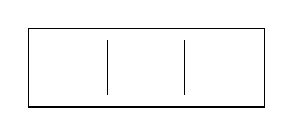
\begin{tikzpicture}[scale=0.7, every node/.style={circle, draw, minimum size=1.2cm}]    
    \node [rectangle, minimum width=3cm, minimum height=1cm, draw] (A) at (0, 0) {};
    \draw (0.7, 0.5) -- (0.7, -0.5);
    \draw (-0.7, 0.5) -- (-0.7, -0.5);
  \end{tikzpicture}
\end{center}

\subsubsection{B木の実装}

\begin{lstlisting}[caption=B木の実装, label=btree, frame=TRBL, label={btree}]
from bisect import bisect_left, bisect_right

class Node:
    def __init__(self):
        self.keys: list[int] = []
        self.children: list[Node] = []

class BTree:
    def __init__(self, order: int) -> None:
        self.order = order
        self.root = Node()
    
    def _median(self, array: list[int]) -> int:
        return array[len(array) // 2]

    def insert(self, value: int) -> None:
        node = self._insert_recursively(self.root, value)
        if node:
            new_root = Node()
            new_root.keys = [node[0]]
            new_root.children = [node[1], node[2]]
            self.root = new_root
    
    def _insert_recursively(self, node: Node, value: int):
        # 葉ノード
        if not node.children:
            node.keys.append(value)
            node.keys.sort()
            if len(node.keys) < self.order:
                return None 
            else:
                return self._split(node)
        else:  
            index = bisect_right(node.keys, value)
            result = self._insert_recursively(node.children[index], value)
            
            if result is not None:
                median, left_node, right_node = result
                node.keys.insert(index, median)
                
                # 修正:左ノードを適切に設定し、右ノードを挿入
                node.children[index] = left_node  # 左の子ノードを置き換える
                node.children.insert(index + 1, right_node)  # 右の子ノードを挿入

                if len(node.keys) < self.order:
                    return None
                else:
                    return self._split(node) 
            return None

    def _split(self, node: Node):
        median_index = len(node.keys) // 2
        median = node.keys[median_index]

        left_node = Node()
        right_node = Node()

        left_node.keys = node.keys[:median_index]
        right_node.keys = node.keys[median_index + 1:]

        if node.children:
            left_node.children = node.children[:median_index + 1]
            right_node.children = node.children[median_index + 1:]

        return median, left_node, right_node

    def search(self, value: int) -> bool:
        node = self.root
        if value in node.keys:
            return True
        else:
            return self._search_recursively(self.root, value)
    
    def _search_recursively(self, node: Node, value: int) -> bool:
        if len(node.children) == 0:
            return False
        
        index = bisect_left(node.keys, value)
        next_node = node.children[index]
        
        if value in next_node.keys:
            return True
        else:
            return self._search_recursively(node.children[index], value)

b_tree = BTree(order=3)
b_tree.insert(5)
b_tree.insert(10)
b_tree.insert(15)
b_tree.insert(20)
b_tree.insert(30)

b_tree.insert(21)
b_tree.insert(22)
\end{lstlisting}

\newpage

\subsection{赤黒木}
赤黒木はAVL木同様平衡二分探索木の1つで、以下の特徴を持っています。

\begin{itemize}
  \item 各ノードは赤か黒の色を持つ
  \item 根ノードは黒である
  \item 赤のノードの子ノードは黒である
  \item あるノードからその子孫の葉ノードまでの黒の数は同じである
  \item 葉ノードは黒である
\end{itemize}


\section{参考}
\textbf{二分探索}

\begin{itemize}
  \item \url{https://qiita.com/drken/items/97e37dd6143e33a64c8c}
\end{itemize}


\noindent \textbf{二分探索木}
\begin{itemize}
  \item \url{https://www.geeksforgeeks.org/introduction-to-avl-tree/}
\end{itemize}

\noindent \textbf{B木}
\begin{itemize}
  \item \url{https://www.geeksforgeeks.org/b-tree-in-python/}
  \item \url{https://www.javatpoint.com/b-tree}
  \item \url{https://wqwq3215.medium.com/b-tree%E3%82%92%E7%90%86%E8%A7%A3%E3%81%97%E3%81%A6%E3%81%84%E3%81%8F-142f93fc3c6c}
\end{itemize}

\noindent \textbf{赤黒木}

\begin{itemize}
  \item \url{https://qiita.com/kgoto/items/b15b9a494deae010d660}
  \item \url{http://wwwa.pikara.ne.jp/okojisan/rb-tree/index.html}
\end{itemize}
\section{力任せ法}
力任せ法は文字通り文字列において、所望のパターンが見つかるまで前から順に比較していく方法です。
以下でtextとpatternの文字列が与えられたときに、textの中にpatternが含まれるかどうか考えましょう。文字列の文字を表す記法は
text[i]のように0-indexで表します。

最初はtext[0]とpattern[0]を比較すると一致しません。一致しないときは、textのcursorを1つ進めてtext[1]とpattern[0]を比較します。

\vspace{0.5cm}
\begin{center}
    \begin{tabular}{|c|c|c|c|c|c|c|c|c|c|c|c|c|}
        \hline
		\makebox[0.5cm]{B} & \makebox[0.5cm]{A} & \makebox[0.5cm]{B} & \makebox[0.5cm]{A} & \makebox[0.5cm]{B} & \makebox[0.5cm]{C} & \makebox[0.5cm]{B} & \makebox[0.5cm]{A} & \makebox[0.5cm]{B} & \makebox[0.5cm]{A} & \makebox[0.5cm]{B} & \makebox[0.5cm]{D} & \makebox[0.5cm]{B} \\ 
        \hline
    \end{tabular}
\end{center}
\begin{center}
    text
\end{center}

\vspace{0.5cm}

% セルの幅を統一した二つ目の表
\begin{center}
    \begin{tabular}{|c|c|c|c|c|c|c|c|c|c|c|c|c|}
        \hline
        \makebox[0.5cm]{A} & \makebox[0.5cm]{B} & \makebox[0.5cm]{A} & \makebox[0.5cm]{B} & \makebox[0.5cm]{D} & \makebox[0.5cm]{} & \makebox[0.5cm]{} & \makebox[0.5cm]{} & \makebox[0.5cm]{} & \makebox[0.5cm]{} & \makebox[0.5cm]{} & \makebox[0.5cm]{} & \makebox[0.5cm]{} \\ 
        \hline
    \end{tabular}
\end{center}
\begin{center}
    pattern
\end{center}

text[1]とpattern[0]を比較すると、一致します。しかし、text[5]とpattern[4]が一致しないので、textのcursorを1つ進めてtext[2]とpattern[0]を比較します。

\vspace{0.5cm}
\begin{center}
    \begin{tabular}{|c|c|c|c|c|c|c|c|c|c|c|c|c|}
        \hline
		\makebox[0.5cm]{B} & \makebox[0.5cm]{A} & \makebox[0.5cm]{B} & \makebox[0.5cm]{A} & \makebox[0.5cm]{B} & \makebox[0.5cm]{C} & \makebox[0.5cm]{B} & \makebox[0.5cm]{A} & \makebox[0.5cm]{B} & \makebox[0.5cm]{A} & \makebox[0.5cm]{B} & \makebox[0.5cm]{D} & \makebox[0.5cm]{B} \\ 
        \hline
    \end{tabular}
\end{center}
\begin{center}
    text
\end{center}

\vspace{0.5cm}

% セルの幅を統一した二つ目の表
\begin{center}
    \begin{tabular}{|c|c|c|c|c|c|c|c|c|c|c|c|c|}
        \hline
        \makebox[0.5cm]{} & \makebox[0.5cm]{A} & \makebox[0.5cm]{B} & \makebox[0.5cm]{A} & \makebox[0.5cm]{B} & \makebox[0.5cm]{D} & \makebox[0.5cm]{} & \makebox[0.5cm]{} & \makebox[0.5cm]{} & \makebox[0.5cm]{} & \makebox[0.5cm]{} & \makebox[0.5cm]{} & \makebox[0.5cm]{} \\ 
        \hline
    \end{tabular}
\end{center}
\begin{center}
    pattern
\end{center}

これを一致していくまで続けていくと、以下のようになります。

\vspace{0.5cm}
\begin{center}
    \begin{tabular}{|c|c|c|c|c|c|c|c|c|c|c|c|c|}
        \hline
        \makebox[0.5cm]{B} & \makebox[0.5cm]{A} & \makebox[0.5cm]{B} & \makebox[0.5cm]{A} & \makebox[0.5cm]{B} & \makebox[0.5cm]{C} & \makebox[0.5cm]{B} & \makebox[0.5cm]{A} & \makebox[0.5cm]{B} & \makebox[0.5cm]{A} & \makebox[0.5cm]{B} & \makebox[0.5cm]{D} & \makebox[0.5cm]{B} \\ 
        \hline
    \end{tabular}
\end{center}
\begin{center}
    text
\end{center}

\vspace{0.5cm}

% セルの幅を統一した二つ目の表
\begin{center}
    \begin{tabular}{|c|c|c|c|c|c|c|c|c|c|c|c|c|}
        \hline
        \makebox[0.5cm]{} & \makebox[0.5cm]{} & \makebox[0.5cm]{} & \makebox[0.5cm]{} & \makebox[0.5cm]{} & \makebox[0.5cm]{} & \makebox[0.5cm]{} & \makebox[0.5cm]{A} & \makebox[0.5cm]{B} & \makebox[0.5cm]{A} & \makebox[0.5cm]{B} & \makebox[0.5cm]{D} & \makebox[0.5cm]{} \\ 
        \hline
    \end{tabular}
\end{center}
\begin{center}
    pattern
\end{center}

例を通じて力任せ法では、textを0からtextの長さ - patternの長さまで動かすことで、patternがtextに含まれるかどうかを判定することができます。C言語で
プログラムを書いてみましょう。

\begin{lstlisting}[caption=力任せの実装, label=force, frame=TRBL]
def brute_force(text: str, pattern: str) -> int:
    for text_cursor in range(len(text) - len(pattern) + 1):
        pattern_cursor = 0
        moving_text_cursor = text_cursor
        while pattern_cursor < len(pattern) and text[moving_text_cursor] == pattern[pattern_cursor]:
            pattern_cursor += 1
            moving_text_cursor += 1
        
        if pattern_cursor == len(pattern):
            return text_cursor
    
    return -1
\end{lstlisting}

\section{KMP法}
\subsection{力任せ法の無駄}
\vspace{0.5cm}
\begin{center}
    \begin{tabular}{|c|c|c|c|c|c|c|c|c|c|c|c|c|}
        \hline
		\makebox[0.5cm]{B} & \makebox[0.5cm]{A} & \makebox[0.5cm]{B} & \makebox[0.5cm]{A} & \makebox[0.5cm]{B} & \makebox[0.5cm]{C} & \makebox[0.5cm]{B} & \makebox[0.5cm]{A} & \makebox[0.5cm]{B} & \makebox[0.5cm]{A} & \makebox[0.5cm]{B} & \makebox[0.5cm]{D} & \makebox[0.5cm]{B} \\ 
        \hline
    \end{tabular}
    \begin{tikzpicture}[overlay, scale=0.5]
        \draw[->, thick] (-19.9, -2) -- (-19.9, -1.5);
    \end{tikzpicture}
\end{center}
\begin{center}
    text
\end{center}

\vspace{0.5cm}

% セルの幅を統一した二つ目の表
\begin{center}
    \begin{tabular}{|c|c|c|c|c|c|c|c|c|c|c|c|c|}
        \hline
        \makebox[0.5cm]{} & \makebox[0.5cm]{A} & \makebox[0.5cm]{B} & \makebox[0.5cm]{A} & \makebox[0.5cm]{B} & \makebox[0.5cm]{D} & \makebox[0.5cm]{} & \makebox[0.5cm]{} & \makebox[0.5cm]{} & \makebox[0.5cm]{} & \makebox[0.5cm]{} & \makebox[0.5cm]{} & \makebox[0.5cm]{} \\ 
        \hline
    \end{tabular}
\end{center}
\begin{center}
    pattern
\end{center}

\vspace{1cm}

上の例ではtext[1]から照合を始めてtext[5]で照合が失敗していることがわかります。力任せ法では
次にtext[2]から照合を始めることになりますが、それはtextの方のcursorが一度通った場所を再度通ることになります。このように、力任せ法は
textのcursorが一度通った場所を再び通ることが多いため、無駄が多いといえます。
ただ、上の例ではABABというパターンがあって、ABABの部分が繰り返されていることがわかります。このような繰り返し部分がある場合、
次に照合を始める位置をスキップすることで無駄が省けそうではないでしょうか?下の例では、textのcursorが後戻りすることなく、patternの位置も
前にスキップされています。

\vspace{0.5cm}
\begin{center}
    \begin{tabular}{|c|c|c|c|c|c|c|c|c|c|c|c|c|}
        \hline
		\makebox[0.5cm]{B} & \makebox[0.5cm]{A} & \makebox[0.5cm]{B} & \makebox[0.5cm]{A} & \makebox[0.5cm]{B} & \makebox[0.5cm]{C} & \makebox[0.5cm]{B} & \makebox[0.5cm]{A} & \makebox[0.5cm]{B} & \makebox[0.5cm]{A} & \makebox[0.5cm]{B} & \makebox[0.5cm]{D} & \makebox[0.5cm]{B} \\ 
        \hline
    \end{tabular}
    \begin{tikzpicture}[overlay, scale=0.5]
        \draw[->, thick] (-16.4, -2) -- (-16.4, -1.5);
    \end{tikzpicture}
\end{center}
\begin{center}
    text
\end{center}

\vspace{0.5cm}

% セルの幅を統一した二つ目の表
\begin{center}
    \begin{tabular}{|c|c|c|c|c|c|c|c|c|c|c|c|c|}
        \hline
        \makebox[0.5cm]{} & \makebox[0.5cm]{} & \makebox[0.5cm]{} & \makebox[0.5cm]{A} & \makebox[0.5cm]{B} & \makebox[0.5cm]{A} & \makebox[0.5cm]{B} & \makebox[0.5cm]{D} & \makebox[0.5cm]{} & \makebox[0.5cm]{} & \makebox[0.5cm]{} & \makebox[0.5cm]{} & \makebox[0.5cm]{} \\ 
        \hline
    \end{tabular}
\end{center}
\begin{center}
    pattern
\end{center}

\vspace{1cm}

\subsection{KMP法}
上のスキップを実現する方法の1つにKMP法があります。KMP法の流れを具体例を見て確認します。

\vspace{0.5cm}
\begin{center}
    \begin{tabular}{|c|c|c|c|c|c|c|c|c|c|c|c|c|}
        \hline
		\makebox[0.5cm]{B} & \makebox[0.5cm]{A} & \makebox[0.5cm]{B} & \makebox[0.5cm]{A} & \makebox[0.5cm]{B} & \makebox[0.5cm]{C} & \makebox[0.5cm]{B} & \makebox[0.5cm]{A} & \makebox[0.5cm]{B} & \makebox[0.5cm]{A} & \makebox[0.5cm]{B} & \makebox[0.5cm]{D} & \makebox[0.5cm]{B} \\ 
        \hline
    \end{tabular}
    \begin{tikzpicture}[overlay, scale=0.5]
        \draw[->, thick] (-13.1, -2) -- (-13.1, -1.5);
    \end{tikzpicture}
\end{center}
\begin{center}
    text
\end{center}

\vspace{0.5cm}

% セルの幅を統一した二つ目の表
\begin{center}
    \begin{tabular}{|c|c|c|c|c|c|c|c|c|c|c|c|c|}
        \hline
        \makebox[0.5cm]{} & \makebox[0.5cm]{A} & \makebox[0.5cm]{B} & \makebox[0.5cm]{A} & \makebox[0.5cm]{B} & \makebox[0.5cm]{D} & \makebox[0.5cm]{} & \makebox[0.5cm]{} & \makebox[0.5cm]{} & \makebox[0.5cm]{} & \makebox[0.5cm]{} & \makebox[0.5cm]{} & \makebox[0.5cm]{} \\ 
        \hline
    \end{tabular}
    \begin{tikzpicture}[overlay, scale=0.5]
        \draw[->, thick] (-13.1, -2) -- (-13.1, -1.5);
    \end{tikzpicture}
\end{center}
\begin{center}
    pattern
\end{center}

\vspace{0.5cm}

\begin{center}
    (1)
\end{center}

%%%%%%%%%%%%%%%%%%%%%%%%%%%%%%%%%%%%%%%%%%%%%%%%%%%%%%%%%%%%

\vspace{0.5cm}
\begin{center}
    \begin{tabular}{|c|c|c|c|c|c|c|c|c|c|c|c|c|}
        \hline
		\makebox[0.5cm]{B} & \makebox[0.5cm]{A} & \makebox[0.5cm]{B} & \makebox[0.5cm]{A} & \makebox[0.5cm]{B} & \makebox[0.5cm]{C} & \makebox[0.5cm]{B} & \makebox[0.5cm]{A} & \makebox[0.5cm]{B} & \makebox[0.5cm]{A} & \makebox[0.5cm]{B} & \makebox[0.5cm]{D} & \makebox[0.5cm]{B} \\ 
        \hline
    \end{tabular}
    \begin{tikzpicture}[overlay, scale=0.5]
        \draw[->, thick] (-13.1, -2) -- (-13.1, -1.5);
    \end{tikzpicture}
\end{center}
\begin{center}
    text
\end{center}

\vspace{0.5cm}

\begin{center}
    \begin{tabular}{|c|c|c|c|c|c|c|c|c|c|c|c|c|}
        \hline
        \makebox[0.5cm]{} & \makebox[0.5cm]{} & \makebox[0.5cm]{} & \makebox[0.5cm]{A} & \makebox[0.5cm]{B} & \makebox[0.5cm]{A} & \makebox[0.5cm]{B} & \makebox[0.5cm]{D} & \makebox[0.5cm]{} & \makebox[0.5cm]{} & \makebox[0.5cm]{} & \makebox[0.5cm]{} & \makebox[0.5cm]{} \\ 
        \hline
    \end{tabular}
    \begin{tikzpicture}[overlay, scale=0.5]
        \draw[->, thick] (-13.1, -2) -- (-13.1, -1.5);
    \end{tikzpicture}
\end{center}
\begin{center}
    pattern
\end{center}

\vspace{0.5cm}

\begin{center}
    (2)
\end{center}

\vspace{0.5cm}

%%%%%%%%%%%%%%%%%%%%%%%%%%%%%%%%%%%%%%%%%%%%%%%%%
\vspace{0.5cm}
\begin{center}
    \begin{tabular}{|c|c|c|c|c|c|c|c|c|c|c|c|c|}
        \hline
		\makebox[0.5cm]{B} & \makebox[0.5cm]{A} & \makebox[0.5cm]{B} & \makebox[0.5cm]{A} & \makebox[0.5cm]{B} & \makebox[0.5cm]{C} & \makebox[0.5cm]{B} & \makebox[0.5cm]{A} & \makebox[0.5cm]{B} & \makebox[0.5cm]{A} & \makebox[0.5cm]{B} & \makebox[0.5cm]{D} & \makebox[0.5cm]{B} \\ 
        \hline
    \end{tabular}
    \begin{tikzpicture}[overlay, scale=0.5]
        \draw[->, thick] (-13.1, -2) -- (-13.1, -1.5);
    \end{tikzpicture}
\end{center}
\begin{center}
    text
\end{center}

\vspace{0.5cm}

\begin{center}
    \begin{tabular}{|c|c|c|c|c|c|c|c|c|c|c|c|c|}
        \hline
        \makebox[0.5cm]{} & \makebox[0.5cm]{} & \makebox[0.5cm]{} & \makebox[0.5cm]{} & \makebox[0.5cm]{} & \makebox[0.5cm]{A} & \makebox[0.5cm]{B} & \makebox[0.5cm]{A} & \makebox[0.5cm]{B} & \makebox[0.5cm]{D} & \makebox[0.5cm]{} & \makebox[0.5cm]{} & \makebox[0.5cm]{} \\ 
        \hline
    \end{tabular}
    \begin{tikzpicture}[overlay, scale=0.5]
        \draw[->, thick] (-13.1, -2) -- (-13.1, -1.5);
    \end{tikzpicture}
\end{center}
\begin{center}
    pattern
\end{center}

\vspace{0.5cm}

\begin{center}
    (3)
\end{center}
%%%%%%%%%%%%%%%%%%%%%%%%%%%%%%%%%%%
\vspace{0.5cm}
\begin{center}
    \begin{tabular}{|c|c|c|c|c|c|c|c|c|c|c|c|c|}
        \hline
		\makebox[0.5cm]{B} & \makebox[0.5cm]{A} & \makebox[0.5cm]{B} & \makebox[0.5cm]{A} & \makebox[0.5cm]{B} & \makebox[0.5cm]{C} & \makebox[0.5cm]{B} & \makebox[0.5cm]{A} & \makebox[0.5cm]{B} & \makebox[0.5cm]{A} & \makebox[0.5cm]{B} & \makebox[0.5cm]{D} & \makebox[0.5cm]{B} \\ 
        \hline
    \end{tabular}
    \begin{tikzpicture}[overlay, scale=0.5]
        \draw[->, thick] (-11.1, -2) -- (-11.1, -1.5);
    \end{tikzpicture}
\end{center}
\begin{center}
    text
\end{center}

\vspace{0.5cm}

\begin{center}
    \begin{tabular}{|c|c|c|c|c|c|c|c|c|c|c|c|c|}
        \hline
        \makebox[0.5cm]{} & \makebox[0.5cm]{} & \makebox[0.5cm]{} & \makebox[0.5cm]{} & \makebox[0.5cm]{} & \makebox[0.5cm]{} & \makebox[0.5cm]{A} & \makebox[0.5cm]{B} & \makebox[0.5cm]{A} & \makebox[0.5cm]{B} & \makebox[0.5cm]{D} & \makebox[0.5cm]{} & \makebox[0.5cm]{} \\ 
        \hline
    \end{tabular}
    \begin{tikzpicture}[overlay, scale=0.5]
        \draw[->, thick] (-11.1, -2) -- (-11.1, -1.5);
    \end{tikzpicture}
\end{center}
\begin{center}
    pattern
\end{center}

\vspace{0.5cm}

\begin{center}
    (4)
\end{center}

%%%%%%%%%%%%%%%%%%%%%%%%%
\vspace{0.5cm}
\vspace{0.5cm}
\begin{center}
    \begin{tabular}{|c|c|c|c|c|c|c|c|c|c|c|c|c|}
        \hline
		\makebox[0.5cm]{B} & \makebox[0.5cm]{A} & \makebox[0.5cm]{B} & \makebox[0.5cm]{A} & \makebox[0.5cm]{B} & \makebox[0.5cm]{C} & \makebox[0.5cm]{B} & \makebox[0.5cm]{A} & \makebox[0.5cm]{B} & \makebox[0.5cm]{A} & \makebox[0.5cm]{B} & \makebox[0.5cm]{D} & \makebox[0.5cm]{B} \\ 
        \hline
    \end{tabular}
    \begin{tikzpicture}[overlay, scale=0.5]
        \draw[->, thick] (-9.6, -2) -- (-9.6, -1.5);
    \end{tikzpicture}
\end{center}
\begin{center}
    text
\end{center}

\vspace{0.5cm}

\begin{center}
    \begin{tabular}{|c|c|c|c|c|c|c|c|c|c|c|c|c|}
        \hline
        \makebox[0.5cm]{} & \makebox[0.5cm]{} & \makebox[0.5cm]{} & \makebox[0.5cm]{} & \makebox[0.5cm]{} & \makebox[0.5cm]{} & \makebox[0.5cm]{} & \makebox[0.5cm]{A} & \makebox[0.5cm]{B} & \makebox[0.5cm]{A} & \makebox[0.5cm]{B} & \makebox[0.5cm]{D} & \makebox[0.5cm]{} \\ 
        \hline
    \end{tabular}
    \begin{tikzpicture}[overlay, scale=0.5]
        \draw[->, thick] (-9.6, -2) -- (-9.6, -1.5);
    \end{tikzpicture}
\end{center}
\begin{center}
    pattern
\end{center}

\vspace{0.5cm}

\begin{center}
    (5) 一致
\end{center}

\vspace{0.5cm}

(1)ではpattern[4]で照合失敗しており、pattern[0]からpattern[3](ABAB)の前半とtext[1]からtext[4]の(ABAB)の後半2文字が一致しています。つまり、
最初の2文字は比べなくても一致していることがわかります。そのため(2)ではpatternのcursorをpatten[2]にして照合を開始しています。

(2)では文字が一致しておらず、patternをずらしてもtext[4], ,text[5]には一致しないので、(3)ではpatternのcursorをはじめに戻しています。

(3)と(4)では文字が一致しておらず、さらにpatternもこれ以上右にシフトすることができないので、textとpatternともに最初の位置からcursorを開始しています。

(5)ではpatternがtextに含まれていることがわかりました。

上の例で見たtextとpatternで一致しているときに飛ばせるcursorの数はpatternによって事前に決まります。そのため、文字列照合の前に\textbf{スキップテーブル}作成を
前処理として行います。

スキップテーブルは以下の条件を満たします。

\begin{itemize}
    \item スキップテーブルの配列の長さはpatternの長さ - 1
    \item スキップテーブルのi番目の要素は、patternのi番目までの部分文字列の最大の接頭辞と接尾辞の長さ、つまりpattern[0]からpattern[i]までの文字列を見たとき、
    前から何文字目までが後ろから何文字目までと一致しているかを表す。
    \item スキップテーブルの最初の要素は0
\end{itemize}

\vspace{0.1cm}

スキップテーブルを作成するには、pattern同士をずらして比べていきます。その際に以下の手順で作成します。

\begin{itemize}
    \item 文字がマッチする場合は、直近の最長部分一致の長さを記録し、そのまま照合を次の文字に進める
    \item 文字がマッチしない場合は、マッチが失敗した位置からパターンの中で可能な部分一致の場所に移動する(KMP法そのもの)
\end{itemize}

%%%%%%%%%%%%%%%%%%%%%%%%%%%%%%%%%%%%%%%%%%%%%%%%%%%%%%%%%%%%%
\vspace{0.5cm}
\begin{center}
    \begin{tabular}{|c|c|c|c|c|c|c|c|c|c|c|c|c|c|}
        \hline
        \makebox[0.5cm]{B} & \makebox[0.5cm]{A} & \makebox[0.5cm]{B} & \makebox[0.5cm]{A} & \makebox[0.5cm]{B} & \makebox[0.5cm]{C} & \makebox[0.5cm]{B} & \makebox[0.5cm]{A} & \makebox[0.5cm]{B} & \makebox[0.5cm]{A} & \makebox[0.5cm]{B} & \makebox[0.5cm]{D} & \makebox[0.5cm]{B} & \makebox[0.5cm]{} \\ 
        \hline
    \end{tabular}
\end{center}
\begin{center}
    \begin{tabular}{|c|c|c|c|c|c|c|c|c|c|c|c|c|c|}
        \hline
        \makebox[0.5cm]{} & \makebox[0.5cm]{B} & \makebox[0.5cm]{A} & \makebox[0.5cm]{B} & \makebox[0.5cm]{A} & \makebox[0.5cm]{B} & \makebox[0.5cm]{C} & \makebox[0.5cm]{B} & \makebox[0.5cm]{A} & \makebox[0.5cm]{B} & \makebox[0.5cm]{A} & \makebox[0.5cm]{B} & \makebox[0.5cm]{D} & \makebox[0.5cm]{B} \\ 
        \hline
    \end{tabular}
\end{center}

\begin{center}
    pattern
\end{center}

\vspace{0.5cm}
%%%%%%%%%%%%%%%%%%%%%%%%%%%%%%%%%%%%%%%%%%%%%%%%%%%%%%%%%%%%%

pattern[1]とpattern[0]から照合を開始します。pattern[1]で照合が失敗しました。pattern[0]で失敗するとpatternを動かせないので
skip[1]に0を入れてcursorを進めます。

\vspace{0.5cm}
\begin{center}
    \begin{tabular}{|c|c|c|c|c|c|c|c|c|c|c|c|}
        \hline
        \makebox[0.5cm]{0} & \makebox[0.5cm]{0} & \makebox[0.5cm]{} & \makebox[0.5cm]{} & \makebox[0.5cm]{} & \makebox[0.5cm]{} & \makebox[0.5cm]{} & \makebox[0.5cm]{} & \makebox[0.5cm]{} & \makebox[0.5cm]{} & \makebox[0.5cm]{} & \makebox[0.5cm]{} \\ 
        \hline
    \end{tabular}

    % boxの下にindexを振る
    \begin{tikzpicture}[overlay, remember picture]
        \foreach \i [count=\n from 1] in {0, 1, 2, 3, 4, 5, 6, 7, 8, 9, 10, 11} {
            \node at ({\n * 0.85 - 5.55}, 0) {\i};
        }
    \end{tikzpicture}

    \begin{center}
        skip
    \end{center}
\end{center}

\vspace{0.5cm}

次はpattern[2]とpattern[0]を照合します。今回は文字が一致しているため、0 + 1をしてskip[2]に1を入れてcursorを進めます。
また、pattern[3]とpattern[1]、pattern[4]とpattern[2]も一致しているため、skip[3]とskip[4]にはそれぞれ2と3を入れます。

%%%%%%%%%%%%%%%%%%%%%%%%%
\vspace{0.5cm}
\begin{center}
    \begin{tabular}{|c|c|c|c|c|c|c|c|c|c|c|c|c|c|c|}
        \hline
        \makebox[0.5cm]{B} & \makebox[0.5cm]{A} & \makebox[0.5cm]{B} & \makebox[0.5cm]{A} & \makebox[0.5cm]{B} & \makebox[0.5cm]{C} & \makebox[0.5cm]{B} & \makebox[0.5cm]{A} & \makebox[0.5cm]{B} & \makebox[0.5cm]{A} & \makebox[0.5cm]{B} & \makebox[0.5cm]{D} & \makebox[0.5cm]{B} & \makebox[0.5cm]{}  & \makebox[0.5cm]{}  \\ 
        \hline
    \end{tabular}
\end{center}
\begin{center}
    \begin{tabular}{|c|c|c|c|c|c|c|c|c|c|c|c|c|c|c|}
        \hline
        \makebox[0.5cm]{} &\makebox[0.5cm]{} & \makebox[0.5cm]{B} & \makebox[0.5cm]{A} & \makebox[0.5cm]{B} & \makebox[0.5cm]{A} & \makebox[0.5cm]{B} & \makebox[0.5cm]{C} & \makebox[0.5cm]{B} & \makebox[0.5cm]{A} & \makebox[0.5cm]{B} & \makebox[0.5cm]{A} & \makebox[0.5cm]{B} & \makebox[0.5cm]{D} & \makebox[0.5cm]{B} \\ 
        \hline
    \end{tabular}
\end{center}

\begin{center}
    pattern
\end{center}

\vspace{0.5cm}
%%%%%%%%%%%%%%%%%%%%%%%%%%%%%%%%%%%%%%%%%%%%%%%%%%%%%%%%%%%%%

\vspace{0.5cm}
\begin{center}
    \begin{tabular}{|c|c|c|c|c|c|c|c|c|c|c|c|}
        \hline
        \makebox[0.5cm]{0} & \makebox[0.5cm]{0} & \makebox[0.5cm]{1} & \makebox[0.5cm]{2} & \makebox[0.5cm]{3} & \makebox[0.5cm]{} & \makebox[0.5cm]{} & \makebox[0.5cm]{} & \makebox[0.5cm]{} & \makebox[0.5cm]{} & \makebox[0.5cm]{} & \makebox[0.5cm]{} \\ 
        \hline
    \end{tabular}

    % boxの下にindexを振る
    \begin{tikzpicture}[overlay, remember picture]
        \foreach \i [count=\n from 1] in {0, 1, 2, 3, 4, 5, 6, 7, 8, 9, 10, 11} {
            \node at ({\n * 0.85 - 5.55}, 0) {\i};
        }
    \end{tikzpicture}

    \begin{center}
        skip
    \end{center}
\end{center}

\vspace{0.5cm}

pattern[5]とpattern[3]は一致していません。マッチが失敗した位置からパターンの中で可能な部分一致の場所
に移動するつまり、skip[3-1] = skip[2]の1にします。

\vspace{0.5cm}
\begin{center}
    \begin{tabular}{|c|c|c|c|c|c|c|c|c|c|c|c|c|c|c|c|c|}
        \hline
        \makebox[0.5cm]{B} & \makebox[0.5cm]{A} & \makebox[0.5cm]{B} & \makebox[0.5cm]{A} & \makebox[0.5cm]{B} & \makebox[0.5cm]{C} & \makebox[0.5cm]{B} & \makebox[0.5cm]{A} & \makebox[0.5cm]{B} & \makebox[0.5cm]{A} & \makebox[0.5cm]{B} & \makebox[0.5cm]{D} & \makebox[0.5cm]{B} & \makebox[0.5cm]{}  & \makebox[0.5cm]{} & \makebox[0.5cm]{} & \makebox[0.5cm]{} \\ 
        \hline
    \end{tabular}
\end{center}
\begin{center}
    \begin{tabular}{|c|c|c|c|c|c|c|c|c|c|c|c|c|c|c|c|c|}
        \hline
        \makebox[0.5cm]{} & \makebox[0.5cm]{} &\makebox[0.5cm]{} &\makebox[0.5cm]{} & \makebox[0.5cm]{B} & \makebox[0.5cm]{A} & \makebox[0.5cm]{B} & \makebox[0.5cm]{A} & \makebox[0.5cm]{B} & \makebox[0.5cm]{C} & \makebox[0.5cm]{B} & \makebox[0.5cm]{A} & \makebox[0.5cm]{B} & \makebox[0.5cm]{A} & \makebox[0.5cm]{B} & \makebox[0.5cm]{D} & \makebox[0.5cm]{B}\\ 
        \hline
    \end{tabular}
\end{center}

\begin{center}
    pattern
\end{center}

\vspace{0.5cm}
比較せずともpattern[4]とpattern[0]は一致していることに注意をしてください。ただ。pattern[5]とpattern[1]で比較して失敗しているので、skip[1-1]を見てpatternを0から開始に移動します。
%%%%%%%%%%%%%%%%%%%%%%%%%%%%%%%%%%%%%%%%%%%%%%%%%%%
\vspace{0.5cm}
\begin{center}
    \begin{tabular}{|c|c|c|c|c|c|c|c|c|c|c|c|c|c|c|c|c|c|}
        \hline
        \makebox[0.5cm]{B} & \makebox[0.5cm]{A} & \makebox[0.5cm]{B} & \makebox[0.5cm]{A} & \makebox[0.5cm]{B} & \makebox[0.5cm]{C} & \makebox[0.5cm]{B} & \makebox[0.5cm]{A} & \makebox[0.5cm]{B} & \makebox[0.5cm]{A} & \makebox[0.5cm]{B} & \makebox[0.5cm]{D} & \makebox[0.5cm]{B} & \makebox[0.5cm]{}  & \makebox[0.5cm]{} & \makebox[0.5cm]{} & \makebox[0.5cm]{}  & \makebox[0.5cm]{}\\ 
        \hline
    \end{tabular}
\end{center}
\begin{center}
    \begin{tabular}{|c|c|c|c|c|c|c|c|c|c|c|c|c|c|c|c|c|c|}
        \hline
        \makebox[0.5cm]{} & \makebox[0.5cm]{} & \makebox[0.5cm]{} &\makebox[0.5cm]{} &\makebox[0.5cm]{} & \makebox[0.5cm]{B} & \makebox[0.5cm]{A} & \makebox[0.5cm]{B} & \makebox[0.5cm]{A} & \makebox[0.5cm]{B} & \makebox[0.5cm]{C} & \makebox[0.5cm]{B} & \makebox[0.5cm]{A} & \makebox[0.5cm]{B} & \makebox[0.5cm]{A} & \makebox[0.5cm]{B} & \makebox[0.5cm]{D} & \makebox[0.5cm]{B}\\ 
        \hline
    \end{tabular}
\end{center}

\begin{center}
    pattern
\end{center}
%%%%%%%%%%%%%%%%%%%%%%%%%%%%%%%%%%%%%%%%%%%%%%%%%%%

\vspace{0.5cm}
下のpatternを移動できるだけ移動しても一致していないので、skip[5]には0を入れて再びcursorを前に移動させます。下の図のように次に移動すると上のpattern[10]までは
一致していることがわかるので、skipを同様に埋めてしまいます。

\vspace{0.5cm}
\begin{center}
    \begin{tabular}{|c|c|c|c|c|c|c|c|c|c|c|c|c|c|c|c|c|c|c|}
        \hline
        \makebox[0.5cm]{B} & \makebox[0.5cm]{A} & \makebox[0.5cm]{B} & \makebox[0.5cm]{A} & \makebox[0.5cm]{B} & \makebox[0.5cm]{C} & \makebox[0.5cm]{B} & \makebox[0.5cm]{A} & \makebox[0.5cm]{B} & \makebox[0.5cm]{A} & \makebox[0.5cm]{B} & \makebox[0.5cm]{D} & \makebox[0.5cm]{B} & \makebox[0.5cm]{}  & \makebox[0.5cm]{} & \makebox[0.5cm]{} & \makebox[0.5cm]{} & \makebox[0.5cm]{} & \makebox[0.5cm]{}\\ 
        \hline
    \end{tabular}
\end{center}
\begin{center}
    \begin{tabular}{|c|c|c|c|c|c|c|c|c|c|c|c|c|c|c|c|c|c|c|}
        \hline
        \makebox[0.5cm]{} & \makebox[0.5cm]{} &\makebox[0.5cm]{} & \makebox[0.5cm]{} &\makebox[0.5cm]{} &\makebox[0.5cm]{} & \makebox[0.5cm]{B} & \makebox[0.5cm]{A} & \makebox[0.5cm]{B} & \makebox[0.5cm]{A} & \makebox[0.5cm]{B} & \makebox[0.5cm]{C} & \makebox[0.5cm]{B} & \makebox[0.5cm]{A} & \makebox[0.5cm]{B} & \makebox[0.5cm]{A} & \makebox[0.5cm]{B} & \makebox[0.5cm]{D} & \makebox[0.5cm]{B}\\ 
        \hline
    \end{tabular}
\end{center}

\begin{center}
    pattern
\end{center}

\vspace{0.5cm}
\begin{center}
    \begin{tabular}{|c|c|c|c|c|c|c|c|c|c|c|c|}
        \hline
        \makebox[0.5cm]{0} & \makebox[0.5cm]{0} & \makebox[0.5cm]{1} & \makebox[0.5cm]{2} & \makebox[0.5cm]{3} & \makebox[0.5cm]{0} & \makebox[0.5cm]{1} & \makebox[0.5cm]{2} & \makebox[0.5cm]{3} & \makebox[0.5cm]{4} & \makebox[0.5cm]{5} & \makebox[0.5cm]{} \\ 
        \hline
    \end{tabular}

    % boxの下にindexを振る
    \begin{tikzpicture}[overlay, remember picture]
        \foreach \i [count=\n from 1] in {0, 1, 2, 3, 4, 5, 6, 7, 8, 9, 10, 11} {
            \node at ({\n * 0.85 - 5.55}, 0) {\i};
        }
    \end{tikzpicture}

    \begin{center}
        skip
    \end{center}
\end{center}

pattern[11]とpattern[5]を比較すると一致していないので、skip[5-1] = skip[4]を見ると3になっているので下のpatternの照合位置を4からにします。

\vspace{0.5cm}
\begin{center}
    \begin{tabular}{|c|c|c|c|c|c|c|c|c|c|c|c|c|c|c|c|c|c|c|c|c|c|}
        \hline
        \makebox[0.5cm]{B} & \makebox[0.5cm]{A} & \makebox[0.5cm]{B} & \makebox[0.5cm]{A} & \makebox[0.5cm]{B} & \makebox[0.5cm]{C} & \makebox[0.5cm]{B} & \makebox[0.5cm]{A} & \makebox[0.5cm]{B} & \makebox[0.5cm]{A} & \makebox[0.5cm]{B} & \makebox[0.5cm]{D} & \makebox[0.5cm]{B} & \makebox[0.5cm]{}  & \makebox[0.5cm]{} & \makebox[0.5cm]{} & \makebox[0.5cm]{} & \makebox[0.5cm]{} & \makebox[0.5cm]{} & \makebox[0.5cm]{} & \makebox[0.5cm]{} & \makebox[0.5cm]{}\\ 
        \hline
    \end{tabular}
\end{center}
\begin{center}
    \begin{tabular}{|c|c|c|c|c|c|c|c|c|c|c|c|c|c|c|c|c|c|c|c|c|c|c}
        \hline
        \makebox[0.5cm]{} & \makebox[0.5cm]{} &\makebox[0.5cm]{} & \makebox[0.5cm]{} &\makebox[0.5cm]{} & \makebox[0.5cm]{} &\makebox[0.5cm]{} &\makebox[0.5cm]{} & \makebox[0.5cm]{B} & \makebox[0.5cm]{A} & \makebox[0.5cm]{B} & \makebox[0.5cm]{A} & \makebox[0.5cm]{B} & \makebox[0.5cm]{C} & \makebox[0.5cm]{B} & \makebox[0.5cm]{A} & \makebox[0.5cm]{B} & \makebox[0.5cm]{A} & \makebox[0.5cm]{B} & \makebox[0.5cm]{D} & \makebox[0.5cm]{B} & \makebox[0.5cm]{} \\ 
        \hline
    \end{tabular}
\end{center}

\begin{center}
    pattern
\end{center}

\vspace{0.5cm}

pattern[11](D)とpattern[3](A)はまたもや一致していないので、skip[3-1] = skip[2]を見ると1になっているので、下のpatternの照合位置を1からにします。

%%%%%%%%%%%%%%%%%%%%%%%%%%%%%%%%%%%%%%%%%%%%%%%%%%%
\vspace{0.5cm}
\begin{center}
    \begin{tabular}{|c|c|c|c|c|c|c|c|c|c|c|c|c|c|c|c|c|c|c|c|c|c|}
        \hline
        \makebox[0.5cm]{B} & \makebox[0.5cm]{A} & \makebox[0.5cm]{B} & \makebox[0.5cm]{A} & \makebox[0.5cm]{B} & \makebox[0.5cm]{C} & \makebox[0.5cm]{B} & \makebox[0.5cm]{A} & \makebox[0.5cm]{B} & \makebox[0.5cm]{A} & \makebox[0.5cm]{B} & \makebox[0.5cm]{D} & \makebox[0.5cm]{B} & \makebox[0.5cm]{}  & \makebox[0.5cm]{} & \makebox[0.5cm]{} & \makebox[0.5cm]{} & \makebox[0.5cm]{} & \makebox[0.5cm]{} & \makebox[0.5cm]{} & \makebox[0.5cm]{} & \makebox[0.5cm]{}\\ 
        \hline
    \end{tabular}
\end{center}
\begin{center}
    \begin{tabular}{|c|c|c|c|c|c|c|c|c|c|c|c|c|c|c|c|c|c|c|c|c|c|c|c|}
        \hline
        \makebox[0.5cm]{} &\makebox[0.5cm]{} &\makebox[0.5cm]{} & \makebox[0.5cm]{} &\makebox[0.5cm]{} & \makebox[0.5cm]{} &\makebox[0.5cm]{} & \makebox[0.5cm]{} &\makebox[0.5cm]{} &\makebox[0.5cm]{} & \makebox[0.5cm]{B} & \makebox[0.5cm]{A} & \makebox[0.5cm]{B} & \makebox[0.5cm]{A} & \makebox[0.5cm]{B} & \makebox[0.5cm]{C} & \makebox[0.5cm]{B} & \makebox[0.5cm]{A} & \makebox[0.5cm]{B} & \makebox[0.5cm]{A} & \makebox[0.5cm]{B} & \makebox[0.5cm]{D} & \makebox[0.5cm]{B} & \makebox[0.5cm]{} \\ 
        \hline
    \end{tabular}
\end{center}

\begin{center}
    pattern
\end{center}
%%%%%%%%%%%%%%%%%%%%%%%%%%%%%%%%%%%%%%%%%%%%%%%%%%%
またまたpattern[11]とpattern[1]は一致しておらず、もうpatternの移動する余裕はないのでskip[10]には0を入れます。

\vspace{0.5cm}
\begin{center}
    \begin{tabular}{|c|c|c|c|c|c|c|c|c|c|c|c|}
        \hline
        \makebox[0.5cm]{0} & \makebox[0.5cm]{0} & \makebox[0.5cm]{1} & \makebox[0.5cm]{2} & \makebox[0.5cm]{3} & \makebox[0.5cm]{0} & \makebox[0.5cm]{1} & \makebox[0.5cm]{2} & \makebox[0.5cm]{3} & \makebox[0.5cm]{4} & \makebox[0.5cm]{5} & \makebox[0.5cm]{0}\\ 
        \hline
    \end{tabular}

    % boxの下にindexを振る
    \begin{tikzpicture}[overlay, remember picture]
        \foreach \i [count=\n from 1] in {0, 1, 2, 3, 4, 5, 6, 7, 8, 9, 10, 11} {
            \node at ({\n * 0.85 - 5.55}, 0) {\i};
        }
    \end{tikzpicture}

    \begin{center}
        skip
    \end{center}
\end{center}

\vspace{0.5cm}
これでスキップテーブルは完成です。好きな文字列と上の例で扱った文字列を照合してみると理解が深まります。

実装のポイントは以下の2つです。

\begin{itemize}
    \item スキップテーブルの作成
    \item 前処理で用意したスキップテーブルを使った文字列照合
\end{itemize}

\begin{lstlisting}[caption=KMP法の実装, frame=TRBL, label={KMP}]
def create_table(pattern: str) -> list[int]:
    skip = [0] * (len(pattern) - 1)
    j = 0

    for i in range(1, len(pattern) - 1):
        if pattern[i] == pattern[j]:
            j += 1
            skip[i] = j
        else:
            while j > 0 and pattern[i] != pattern[j]:
                j = skip[j-1]
            
            # 例によっては忘れがちなので注意
            if pattern[i] == pattern[j]:
                j += 1
            
            skip[i] = j
    
    return skip

def kmp(text: str, patten: str) -> int:
    skip_table = create_table(patten)
    pattern_cursor = 0
    # len(text) - len(pattern) + 1ではないことに注意
    for text_cursor in range(len(text)):
        if text[text_cursor] == patten[pattern_cursor]:
            pattern_cursor += 1
        else:
            while pattern_cursor > 0 and text[text_cursor] != patten[pattern_cursor]:
                pattern_cursor = skip_table[pattern_cursor - 1]
            
            if text[text_cursor] == pattern[pattern_cursor]:
                pattern_cursor += 1
                
        
        if pattern_cursor == len(patten):
            return text_cursor - len(patten) + 1
        
    return - 1
\end{lstlisting}

\newpage

\section{BM法}
\subsection{BM法の仕組み}
BM法は照合パターンの前からではなくて、後ろから照合を開始します。照合パターンの一番最後つまりDから照合を開始
します。CとDは一致していないので、ずらします。
\vspace{0.5cm}
\begin{center}
    \begin{tabular}{|c|c|c|c|c|c|c|c|c|c|c|c|c|c|c|c|}
        \hline
        \makebox[0.5cm]{B} & \makebox[0.5cm]{A} & \makebox[0.5cm]{B} & \makebox[0.5cm]{A} & \makebox[0.5cm]{C} & \makebox[0.5cm]{C} & \makebox[0.5cm]{B} & \makebox[0.5cm]{A} & \makebox[0.5cm]{B} & \makebox[0.5cm]{A} & \makebox[0.5cm]{B} & \makebox[0.5cm]{A} & \makebox[0.5cm]{B}  & \makebox[0.5cm]{D} & \makebox[0.5cm]{B}\\ 
        \hline
    \end{tabular}
\end{center}
\begin{center}
    \begin{tabular}{|c|c|c|c|c|c|c|c|c|c|c|c|c|c|c|c|}
        \hline
        \makebox[0.5cm]{A} & \makebox[0.5cm]{B} & \makebox[0.5cm]{A} & \makebox[0.5cm]{B} & \makebox[0.5cm]{D} & \makebox[0.5cm]{} & \makebox[0.5cm]{} & \makebox[0.5cm]{} & \makebox[0.5cm]{} & \makebox[0.5cm]{} & \makebox[0.5cm]{} & \makebox[0.5cm]{}  & \makebox[0.5cm]{} & \makebox[0.5cm]{} & \makebox[0.5cm]{}\\ 
        \hline
    \end{tabular}
\end{center}
\vspace{0.5cm}

BM法では以下のように最初から多くスキップすることが多いです。

\vspace{0.5cm}

\begin{center}
    \begin{tabular}{|c|c|c|c|c|c|c|c|c|c|c|c|c|c|c|c|}
        \hline
        \makebox[0.5cm]{B} & \makebox[0.5cm]{A} & \makebox[0.5cm]{B} & \makebox[0.5cm]{A} & \makebox[0.5cm]{C} & \makebox[0.5cm]{C} & \makebox[0.5cm]{B} & \makebox[0.5cm]{A} & \makebox[0.5cm]{B} & \makebox[0.5cm]{A} & \makebox[0.5cm]{B} & \makebox[0.5cm]{A} & \makebox[0.5cm]{B}  & \makebox[0.5cm]{D} & \makebox[0.5cm]{B}\\ 
        \hline
    \end{tabular}
\end{center}
\begin{center}
    \begin{tabular}{|c|c|c|c|c|c|c|c|c|c|c|c|c|c|c|c|}
        \hline
        \makebox[0.5cm]{} & \makebox[0.5cm]{} & \makebox[0.5cm]{} & \makebox[0.5cm]{} & \makebox[0.5cm]{} & \makebox[0.5cm]{A} & \makebox[0.5cm]{B} & \makebox[0.5cm]{A} & \makebox[0.5cm]{B} & \makebox[0.5cm]{D} & \makebox[0.5cm]{} & \makebox[0.5cm]{}  & \makebox[0.5cm]{} & \makebox[0.5cm]{} & \makebox[0.5cm]{}\\ 
        \hline
    \end{tabular}
\end{center}
\vspace{0.5cm}

またAとDは一致していないのでスキップします。今回はAという文字で照合が失敗していますが、照合パターンにもAがあるので先ほどのように一気に飛ばせません。

\vspace{0.5cm}

\begin{center}
    \begin{tabular}{|c|c|c|c|c|c|c|c|c|c|c|c|c|c|c|c|}
        \hline
        \makebox[0.5cm]{B} & \makebox[0.5cm]{A} & \makebox[0.5cm]{B} & \makebox[0.5cm]{A} & \makebox[0.5cm]{C} & \makebox[0.5cm]{C} & \makebox[0.5cm]{B} & \makebox[0.5cm]{A} & \makebox[0.5cm]{B} & \makebox[0.5cm]{A} & \makebox[0.5cm]{B} & \makebox[0.5cm]{A} & \makebox[0.5cm]{B}  & \makebox[0.5cm]{D} & \makebox[0.5cm]{B}\\ 
        \hline
    \end{tabular}
\end{center}
\begin{center}
    \begin{tabular}{|c|c|c|c|c|c|c|c|c|c|c|c|c|c|c|c|}
        \hline
        \makebox[0.5cm]{} & \makebox[0.5cm]{} & \makebox[0.5cm]{} & \makebox[0.5cm]{} & \makebox[0.5cm]{} & \makebox[0.5cm]{} & \makebox[0.5cm]{} & \makebox[0.5cm]{A} & \makebox[0.5cm]{B} & \makebox[0.5cm]{A} & \makebox[0.5cm]{B} & \makebox[0.5cm]{D}  & \makebox[0.5cm]{} & \makebox[0.5cm]{} & \makebox[0.5cm]{}\\ 
        \hline
    \end{tabular}
\end{center}
\vspace{0.5cm}

次も同様に考えると以下のようになり、一致します。

\vspace{0.5cm}

\begin{center}
    \begin{tabular}{|c|c|c|c|c|c|c|c|c|c|c|c|c|c|c|c|}
        \hline
        \makebox[0.5cm]{B} & \makebox[0.5cm]{A} & \makebox[0.5cm]{B} & \makebox[0.5cm]{A} & \makebox[0.5cm]{C} & \makebox[0.5cm]{C} & \makebox[0.5cm]{B} & \makebox[0.5cm]{A} & \makebox[0.5cm]{B} & \makebox[0.5cm]{A} & \makebox[0.5cm]{B} & \makebox[0.5cm]{A} & \makebox[0.5cm]{B}  & \makebox[0.5cm]{D} & \makebox[0.5cm]{B}\\ 
        \hline
    \end{tabular}
\end{center}
\begin{center}
    \begin{tabular}{|c|c|c|c|c|c|c|c|c|c|c|c|c|c|c|c|}
        \hline
        \makebox[0.5cm]{} & \makebox[0.5cm]{} & \makebox[0.5cm]{} & \makebox[0.5cm]{} & \makebox[0.5cm]{} & \makebox[0.5cm]{} & \makebox[0.5cm]{} & \makebox[0.5cm]{} & \makebox[0.5cm]{} & \makebox[0.5cm]{A} & \makebox[0.5cm]{B} & \makebox[0.5cm]{A}  & \makebox[0.5cm]{B} & \makebox[0.5cm]{D} & \makebox[0.5cm]{}\\ 
        \hline
    \end{tabular}
\end{center}
\vspace{0.5cm}

上の例では、照合パターンの最後の文字から照合を開始しました。その際にtextで一致しない文字に応じてtextの照合cursorの位置を動かしていました。では、その動かす
大きさはどのように決まるでしょうか?KMP法と同様にスキップテーブルを作成します。スキップテーブルを以下のポイントを意識して作成します。
照合パターンの長さを$l$とします。

\begin{itemize}
    \item パターンに含まれない文字とパターンの一番最後にしかない文字の移動量は$l$
    \item 一番最後以外に含まれる文字に関しては、末尾に最も近い出現位置が$i (0 \leq i < l)$ならば、そのときの移動量は$l - i + 1$
    \item 移動量はtextに出現する文字をすべて網羅する辞書で管理
\end{itemize}

text照合中にどの文字で失敗したかに応じて移動量が変化するので、textに登場する文字が文字が予め分かっている必要があります。textに登場する文字に応じてUS-ASCIIやUTF-8
などの文字コードを使って辞書を作成します。今回はUS-ASCIIで実装します。

\subsection{パターンテーブルだけの実装の問題点}
実はパターンテーブルだけでは問題が起こることがあります。プログラムの停止性に関わる問題です。例えば以下のようなtextとpatternを考えます。

\vspace{0.5cm}

\begin{center}
    \begin{tabular}{|c|c|c|c|c|c|c|c|c|c|c|c|c|c|c|c|}
        \hline
        \makebox[0.5cm]{} & \makebox[0.5cm]{} & \makebox[0.5cm]{} & \makebox[0.5cm]{} & \makebox[0.5cm]{B} & \makebox[0.5cm]{A} & \makebox[0.5cm]{D} & \makebox[0.5cm]{D} & \makebox[0.5cm]{D} & \makebox[0.5cm]{B} & \makebox[0.5cm]{} & \makebox[0.5cm]{} & \makebox[0.5cm]{}  & \makebox[0.5cm]{} & \makebox[0.5cm]{}\\ 
        \hline
    \end{tabular}
\end{center}
\begin{center}
    \begin{tabular}{|c|c|c|c|c|c|c|c|c|c|c|c|c|c|c|c|}
        \hline
        \makebox[0.5cm]{} & \makebox[0.5cm]{} & \makebox[0.5cm]{} & \makebox[0.5cm]{} & \makebox[0.5cm]{A} & \makebox[0.5cm]{C} & \makebox[0.5cm]{A} & \makebox[0.5cm]{D} & \makebox[0.5cm]{B} & \makebox[0.5cm]{} & \makebox[0.5cm]{} & \makebox[0.5cm]{}  & \makebox[0.5cm]{} & \makebox[0.5cm]{} & \makebox[0.5cm]{}\\ 
        \hline
    \end{tabular}
\end{center}
\vspace{0.5cm}

マッチテーブルは以下のようです。

\vspace{0.5cm}

\begin{center}
    \begin{tabular}{|c|c|c|c|c|}
        \hline
        \makebox[0.5cm]{A} & \makebox[0.5cm]{B} & \makebox[0.5cm]{C} & \makebox[0.5cm]{D} & \makebox[0.5cm]{E} \\
        \hline
    \end{tabular}

    \begin{tabular}{|c|c|c|c|c|}
        \hline
        \makebox[0.5cm]{2} & \makebox[0.5cm]{5} & \makebox[0.5cm]{3} & \makebox[0.5cm]{1} & \makebox[0.5cm]{5} \\
        \hline
    \end{tabular}
\end{center}

\vspace{0.5cm}

まず、Dで失敗しているのでスキップテーブルのDを見ると1になっています。textの照合開始位置を一つ進めます。

\vspace{0.5cm}

\begin{center}
    \begin{tabular}{|c|c|c|c|c|c|c|c|c|c|c|c|c|c|c|c|}
        \hline
        \makebox[0.5cm]{} & \makebox[0.5cm]{} & \makebox[0.5cm]{} & \makebox[0.5cm]{} & \makebox[0.5cm]{B} & \makebox[0.5cm]{A} & \makebox[0.5cm]{D} & \makebox[0.5cm]{D} & \makebox[0.5cm]{D} & \makebox[0.5cm]{B} & \makebox[0.5cm]{} & \makebox[0.5cm]{} & \makebox[0.5cm]{}  & \makebox[0.5cm]{} & \makebox[0.5cm]{}\\ 
        \hline
    \end{tabular}
\end{center}
\begin{center}
    \begin{tabular}{|c|c|c|c|c|c|c|c|c|c|c|c|c|c|c|c|}
        \hline
        \makebox[0.5cm]{} & \makebox[0.5cm]{} & \makebox[0.5cm]{} & \makebox[0.5cm]{} & \makebox[0.5cm]{} & \makebox[0.5cm]{A} & \makebox[0.5cm]{C} & \makebox[0.5cm]{A} & \makebox[0.5cm]{D} & \makebox[0.5cm]{B} & \makebox[0.5cm]{} & \makebox[0.5cm]{} & \makebox[0.5cm]{}  & \makebox[0.5cm]{} & \makebox[0.5cm]{}\\ 
        \hline
    \end{tabular}
\end{center}

\vspace{0.5cm}

今度もDで失敗しているので、textの照合開始位置を1進めましょう。今回はtextの途中までは照合が成功しているので、+1するのは照合が失敗したindexであることに注意してください。

\vspace{0.5cm}

\begin{center}
    \begin{tabular}{|c|c|c|c|c|c|c|c|c|c|c|c|c|c|c|c|}
        \hline
        \makebox[0.5cm]{} & \makebox[0.5cm]{} & \makebox[0.5cm]{} & \makebox[0.5cm]{} & \makebox[0.5cm]{B} & \makebox[0.5cm]{A} & \makebox[0.5cm]{D} & \makebox[0.5cm]{D} & \makebox[0.5cm]{D} & \makebox[0.5cm]{B} & \makebox[0.5cm]{} & \makebox[0.5cm]{} & \makebox[0.5cm]{}  & \makebox[0.5cm]{} & \makebox[0.5cm]{}\\ 
        \hline
    \end{tabular}
\end{center}
\begin{center}
    \begin{tabular}{|c|c|c|c|c|c|c|c|c|c|c|c|c|c|c|c|}
        \hline
        \makebox[0.5cm]{} & \makebox[0.5cm]{} & \makebox[0.5cm]{} & \makebox[0.5cm]{} & \makebox[0.5cm]{A} & \makebox[0.5cm]{C} & \makebox[0.5cm]{A} & \makebox[0.5cm]{D} & \makebox[0.5cm]{B} & \makebox[0.5cm]{} & \makebox[0.5cm]{} & \makebox[0.5cm]{}  & \makebox[0.5cm]{} & \makebox[0.5cm]{} & \makebox[0.5cm]{}\\ 
        \hline
    \end{tabular}
\end{center}
\vspace{0.5cm}

これは最初に見たパターンと同じになっているため、無限ループが発生しています。問題の原因は、スキップテーブルだけだとtextの照合開始indexが
後戻りすることがあるためです。スキップテーブルを用いることで、照合開始地点よりも前から照合してもパターンと一致することがないことが
保証されているので、そもそも後戻りする意味はないです。つまり、不一致の場合に次の照合開始地点は前の照合開始地点よりも後ろになって欲しいです。

\vspace{0.5cm}

\begin{center}
    \begin{tabular}{|c|c|c|c|c|c|c|c|c|c|c|c|c|c|c|c|}
        \hline
        \makebox[0.5cm]{} & \makebox[0.5cm]{} & \makebox[0.5cm]{} & \makebox[0.5cm]{} & \makebox[0.5cm]{D} & \makebox[0.5cm]{B} & \makebox[0.5cm]{A} & \makebox[0.5cm]{B} & \makebox[0.5cm]{D} & \makebox[0.5cm]{} & \makebox[0.5cm]{} & \makebox[0.5cm]{} & \makebox[0.5cm]{}  & \makebox[0.5cm]{} & \makebox[0.5cm]{}\\ 
        \hline
    \end{tabular}
\end{center}
\begin{center}
    \begin{tabular}{|c|c|c|c|c|c|c|c|c|c|c|c|c|c|c|c|}
        \hline
        \makebox[0.5cm]{} & \makebox[0.5cm]{} & \makebox[0.5cm]{} & \makebox[0.5cm]{} & \makebox[0.5cm]{A} & \makebox[0.5cm]{C} & \makebox[0.5cm]{A} & \makebox[0.5cm]{B} & \makebox[0.5cm]{D} & \makebox[0.5cm]{} & \makebox[0.5cm]{} & \makebox[0.5cm]{}  & \makebox[0.5cm]{} & \makebox[0.5cm]{} & \makebox[0.5cm]{}\\ 
        \hline
    \end{tabular}
\end{center}
\vspace{0.5cm}

上の例では照合失敗を検知するまで4回比較しており、最後に照合した1点のindex + 4の地点から照合を開始しても問題ありません。よってスキップする大きさを決めるには、

\begin{equation*}
    skip\_size = \max(比較回数、スキップテーブルの値)
\end{equation*}

とすれば良いです。

\subsection{BM法の実装}

実装のポイントは以下の通りです。

\begin{itemize}
    \item スキップテーブルの実装
    \item スキップテーブルを利用して文字列照合
\end{itemize}

\begin{lstlisting}[caption=BM法の実装, frame=TRBL, label={BM}]
def bm(text: str, pattern: int) -> int:
	def create_table(pattern: str) -> list[int]:
		skip = [0] * (1 << 7)
		for i in range(1 << 7):
			last_match = -1
			for j in range(len(pattern)):
				if pattern[j] == chr(i):
					last_match = j
			
			if last_match == -1 or last_match == len(pattern) - 1:
				skip[i] = len(pattern)
			else:
				skip[i] = len(pattern) - last_match - 1
		return skip

	skip = create_table(pattern)

	text_cursor = len(pattern) - 1
	
	while text_cursor < len(text):
		moving_text_cursor = text_cursor
		pattern_cursor = len(pattern) - 1
  
		while text[moving_text_cursor] == pattern[pattern_cursor] and pattern_cursor > 0:
			moving_text_cursor -= 1
			pattern_cursor -= 1
   
		if pattern_cursor == 0:
			return text_cursor - len(pattern) + 1
		
		# スキップテーブルを見てtextの参照開始位置を更新
		compared_times = len(pattern) - pattern_cursor
		skip_table_value = skip[ord(text[moving_text_cursor])]
  
		text_cursor += max(skip_table_value, compared_times)
	
	return -1
  
  
text = input()
pattern = input()

print(bm(text, pattern))

\end{lstlisting}

\newpage

\section{ラビン・カープ法(ローリングハッシュ)}

照合パターンとテキストのハッシュを計算し、そのハッシュが一致するか否かで文字列の一致を判定する方法を紹介します。照合パターンの長さを$l$
とすると、ハッシュを利用することで比較の計算量を$O(l)$から$O(1)$へと定数時間にすることが可能です。

ハッシュは以下のように計算します。互いに素な定数$a, h(1 < a < h)$を用意して、照合パターン($p_0 \cdots p_{l-1}$)に対して、

\begin{equation}
    H(P) = (a^{l-1} p_0 + a^{l-2} p_1 + \cdots + a^0 p_{l-1}) \mod h
\end{equation}

テキストの部分文字列(text[0]からtext[l-1])のハッシュも同様に計算して$H(S, 0, l -1)$とすると、
H(P)とH(S, 0, l - 1)が一致するとき、text[0]からtext[l-1]と照合パターンが一致すると考える。もちろんハッシュが衝突する可能性もあるので実際に一致しているか
確認する必要があります
が、今回はハッシュが一致していれば文字列も一致しているとします。

しかし、このハッシュの計算をテキストの大きさだけ計算すると、$O(nl)$の計算量になってしまいます。ここで、テキストのハッシュは$\mod h$を取ったものであるため、

\begin{equation}
    a^{l-1} p_0 + a^{l-2} p_1 + \cdots + a^0 p_{l-1} = H(S, 0, l - 1) + Ah (\text{Aは整数})
\end{equation}

と表せます。

これを利用すると、$H(S, 1, l)$は前の$H(S, 0, l - 1)$を用いて以下のように表せます。

\begin{align}
    H(S, 1, l) &= a^{l-1}s_1 + a^{l-2}s_2 + \cdots + a^0s_l \nonumber\\ 
    &= a(a^{l-2}s_1 + a^{l-3}s_2 + \cdots + a^1s_{l-1}) + s_l \nonumber\\
    &= a(a^{l-1} s_0 + a^{l-2}s_1 + \cdots + a^0 s_{l-1}) - a^{l} s_0 + a^0 s_l \nonumber \\
    &= aH(S, 0, l - 1) - a^{l} s_0 + a^0 s_l 
\end{align}

よって、テキストのそれぞれのハッシュは前のハッシュを利用することで、定数時間で計算できることがわかりました。これを\textbf{ローリングハッシュ}といいます。

\subsection{ラビン・カープ法の実装}

実装のポイントは以下通りです。

\begin{itemize}
    \item $a, h$を適当に決める
    \item 文字を数値に変換する
    \item テキストと照合パターンのハッシュを保持して尺取法のように計算する
\end{itemize}

\newpage

\begin{lstlisting}[caption=ラビン・カープ法の実装, frame=TRBL, label={Rabin-Karp}]
def rolling_hash(text: str, pattern: str) -> list[int]:
    a = 31
    h = 998244353
    
    text_length, pattern_length = len(text), len(pattern)
    text_hash = pattern_hash = 0
    
    # a^lを先に計算 剰余を取らないと実行時間が非常に長くなる
    a_l = 1
    for i in range(pattern_length):
        a_l = (a_l * a) % h
    
    
    # 最初のハッシュを計算する. 式(1)より
    for i in range(pattern_length):
        text_hash = (a * text_hash + ord(text[i])) % h
        pattern_hash = (a * pattern_hash + ord(pattern[i])) % h
    
    for i in range(text_length - pattern_length + 1):
        if pattern_hash == text_hash:
            return i
        
        if i < text_length - pattern_length:
            # テキストのハッシュを更新
            text_hash = (a * text_hash - a_l * ord(text[i]) + ord(text[i + pattern_length])) % h
        
            if text_hash < 0:
                text_hash += h
    
    return -1
\end{lstlisting}

\subsection{問題}

問題1 ABC 276 A - Right

英子文字からなる文字列が与えられます。最後に現れるaのindexを求める問題です。存在しなければ、-1を出力する問題です。力任せ法とPythonの標準ライブラリ
を使って2つの解法を使って解いてみましょう。実際にAtCoderに参加するときなどは、標準ライブラリを使った解法を使うことが多いですが、
勉強中は自分で実装することが大切です。

\begin{lstlisting}[caption=問題1の解答, frame=TRBL, label={problem1}]
def brute_force_last_index(text: str, pattern: str) -> int:
    last_index = -1
    for text_cursor in range(len(text) - len(pattern) + 1):
        pattern_cursor = 0
        moving_text_cursor = text_cursor
        while pattern_cursor < len(pattern) and text[moving_text_cursor] == pattern[pattern_cursor]:
            pattern_cursor += 1
            moving_text_cursor += 1
        
        if pattern_cursor == len(pattern):
            last_index = text_cursor
        
    
    return last_index

text = input()
pattern = "a"

last_index = brute_force_last_index(text, pattern)

print(last_index + 1 if last_index != -1 else last_index)

# 標準ライブラリを使った解法
text = input()
pattern = "a"

last_index = text.rfind(pattern)

print(last_index + 1 if last_index != -1 else last_index)
\end{lstlisting}

問題2 ABC 336 B - CTZ
\begin{lstlisting}[caption=問題2の解答, frame=TRBL, label={problem2}]
def cal_ctz(number: int) -> int:
    bit_size = number.bit_length()
    shift_size = 0
    
    while shift_size < bit_size:
        if number & (1 << shift_size):
            return shift_size
        else:
            shift_size += 1

def main():
    n = int(input())
    ctz = cal_ctz(n)
    
    print(ctz)
        
if __name__ == "__main__":
    main()
\end{lstlisting}

問題 3 yukicoder No.430 文字列検索
ローリングハッシュの練習問題です。

\textbf{参考}
\begin{itemize}
    \item \url{https://blog.hamayanhamayan.com/entry/2016/10/03/083532}
\end{itemize}

問題 ABC 141 E - Who Says a Pun?
ローリングハッシュ + $\alpha$の難しい問題です。
以下の章からは整数を扱います。

\section{最大公約数とユークリッドの互除法}

整数$a, b(a > b)$の最大公約数を求めるには、\textbf{ユークリッドの互除法}を使用します。

\begin{tcolorbox}[enhanced,title=ユークリッドの互除法, 
  attach boxed title to top left, 
  colback=white!95!blue,
  colbacktitle=white!10!blue!50!black,
  drop fuzzy shadow,
  boxrule=0.25mm,
  ]
  $a, b(a > b)$の最大公約数はa \% bとbの最大公約数と等しい。
\end{tcolorbox}

$a, b$の剰余を計算繰り返し計算していって$b$が0になった時の$a$が最大公約数となります。繰り返し同じ計算をするので、\textbf{再帰関数}
を使って実装します。

\begin{lstlisting}[caption=ユークリッドの互助法実装, frame=TRBL, label={euclid}]
def gcd(a: int, b: int) -> int:
  # 終了条件
  if b == 0:
      return a
  
  if a < b:
      a, b = b, a
      
  return gcd(b, a % b)
\end{lstlisting}

最大公約数をアルゴリズムを理解するだけではなくて、図形を使って直感的に理解しましょう。参考に記したけんちょんさんの最大公約数の記事を参考にすると、最大公約数は$n$次元の立方体を考えたときにそれを均等に分割できる最大の立方体の辺の長さとして考えることができます。このように考えると、最大公約数が何を意味しているのかが直感的に理解できるかもしれません。

\subsection{問題}
\textbf{問題1} ABC 118 C - Monsters Battle Royale \\
問題からはすぐには気づきにくいですが、最大公約数を利用します。$n$次元の立方体を考えたときにそれを均等に分ける最大の立方体の辺の長さを求める問題と同じです。配列Aのどの要素もgcd
の倍数になっているので、gcdがこれ以上分割できない最小の辺の長さとなります。どんなに操作を加えても最小の辺の長さは変わりません。このように操作を繰り返しても
変わらない数のことを\textbf{不変量}といいます。与えられた配列Aの要素同士の引き算から必ずgcdを生み出せるかという疑問が生まれるかもしれませんが、
ユークリッドの互除法を使うことで、gcdを求めることができます。

\begin{tcolorbox}[enhanced, title=コラム 再帰関数, breakable, colback=white, drop fuzzy shadow, attach boxed title to top center={yshift*=0.1cm}]
  おそらく初めて再帰関数を見た方は再帰関数の動きがわかりにくいと思います。再帰関数は自分自身を呼び出す関数です。そのため、再帰関数を理解するためには、関数が呼び出された時にどのような動きをするのかを理解する必要があります。
  関数が呼び出されると、スタックに関数が積まれていきます。最初に呼び出したgcdは一番下に、最後に呼び出したgcdはスタックの一番上に置かれます。一番上の関数戻り値がわかったら、連鎖的にそれより下の関数の値もわかります。そして今回の場合シグネチャからもわかる通り、intのデータ型の値を返す関数です。
  returnする箇所で再びintの値を返す関数を呼び出しているので、スタックに積まれた関数がreturnするまで関数が呼び出され続けます。=が
  終了条件を満たすまで連なっていると考えるとわかりやすいかもしれません。
\end{tcolorbox}


\section{拡張ユークリッドの互除法}

ユークリッドの互除法では、最大公約数を求めることができますが、拡張ユークリッドの互除法を使うと、最大公約数だけでなく、$ax + by = \gcd(a, b)$を満たす$x, y$を求めることができます。

$ax + by = gcd(a, b)$の$a, b$に対してユークリッドの互除法を適用していきます。通常のユークリッドの互除法のように、$a \% b, b$を計算していきますが、計算した結果それがれが
次の一次不定方程式の係数となります。$b x_1 + \{(a\%b) y_1\} = gcd(a, b)$となります。ここで、

\begin{equation*}
    a \% b = a - (a//b) \times b
\end{equation*}

が成立することから、代入して

\begin{align*}
    b x_1 + ay_1 - (a//b) \times b y_1 = gcd(a, b) \\
    ay_1 + b(x_1 - (a//b) y_1) = gcd(a, b)
\end{align*}

$a x + b y = gcd(a, b)$と$a, b$について係数比較をすることで、

\begin{equation}
    x = y_1, y = x_1 - (a//b) \times y_1
\end{equation}


$x_1, y_1$は$b, a\%b$に対して再帰的に求めることができます。終了条件は$b = 0$のときで、このときの$x$が求める$x$となります。

具体例を見ましょう。$a = 108, b = 56$つまり$108 x + 56 y = gcd(108, 56)$です。

\begin{align*}
    108 x + 56 y &= gcd(108, 56) \\
    56 x_1 + 52 y_1 &= gcd(56, 52) \\
    52 x_2 + 4 y_2 &= gcd(52, 4) \\
    4 x_3 + 0 y_3 &= gcd(4, 0)
\end{align*}

$a x + by = gcd(a, b)$の解$(x, y)$が$b$と$a\%b$を係数にした一次不定方程式の解$(x_1, y_1)$から求められていることを確認してください。上から順に再帰的に(b, a\%b)を求めています。$b = 0$になったとき、$x_3 = 1, y_3 = 0$になります。式(1)より、
$x_2 = y_3 = 0, y_2 = x_3 - (52//4) \times y_3 = 1$となります。同様に、$x_1 = y_2 = 1, y_1 = x_2 - (56 // 54) y_2 = - 1$

以上より、$x = y_1 = -1, y = x_1 - (108 // 56) \times y_1$ = 2となります。

実装は以下のようになります。

\begin{lstlisting}[caption=拡張ユークリッドの互助法実装, frame=TRBL, label={euclid}]
def extended_gcd(a: int, b: int) -> tuple[int, int, int]:
    if b == 0:
        return a, 1, 0
    else:
        gcd, x1, y1 = extended_gcd(b, a % b)
    
        # 係数の更新
        x = y1
        y = x1 - (a // b) * y1
        
        return gcd, x, y
    

\end{lstlisting}

\textbf{参考}
\begin{itemize}
    \item \url{https://qiita.com/drken/items/0c88a37eec520f82b788}
\end{itemize}

\section{素数判定}

\subsection{ナイーブな実装}

ナイーブな実装では以下の定理を利用して、自然数$n$の素数判定を行います。

\begin{tcolorbox}[enhanced,title=定理1, 
  attach boxed title to top left, 
  colback=white!95!blue,
  colbacktitle=white!10!blue!50!black,
  drop fuzzy shadow,
  boxrule=0.25mm,
  ]
  自然数$n$が$\sqrt{n}$以下の素数で割り切れないならば、$n$は素数である。
\end{tcolorbox}
実装は以下のようになります。

\begin{lstlisting}[caption=ナイーブな素数判定, frame=TRBL, label={naivePriem}]
def is_prime(n: int) -> bool:
    # 忘れないように注意
    if n <= 1:
        return False
    i = 2
    while i * i <= n:
        if n % i == 0:
            return False
        i += 1
    
    return True

\end{lstlisting}

ナイーブな実装では、1個の自然数が素数か判定するには$O(\sqrt{n})$でできますが、$n$個の数を判定するとなったら$O(n \sqrt{n})$かかり少し遅いです。

\subsection{エラトステネスの篩}
多くの自然数の素数判定を高速に行う方法の1つに\textbf{エラトステネスの篩}があります。求める自然数の最大値を$n$とすると、
1から$n$までの自然数の素数判定はエラトステネスの篩を使うと、$O(n \log \log n)$の計算量で実行可能です。

エラトステネスのの篩では、判定したい自然数$n$までのテーブルを作成し、2から順に以下の操作を$\sqrt{n}$まで繰り返します。

\begin{enumerate}
  \item $i = 2$からスタート
  \item iがテーブルでバツがついていない場合、iを除いたiのすべての倍数を素数ではないとする
  \item $i = i + 1$ ($i = \sqrt{n}$まで2へ)
\end{enumerate}

例として$n = 100$の場合を見てみます。

\newpage


\begin{center}
  \begin{tabular}{|c|c|c|c|c|c|c|c|c|c|}
      \hline
      1  & 2  & 3  & 4  & 5  & 6  & 7  & 8  & 9  & 10 \\ \hline
      11 & 12 & 13 & 14 & 15 & 16 & 17 & 18 & 19 & 20 \\ \hline
      21 & 22 & 23 & 24 & 25 & 26 & 27 & 28 & 29 & 30 \\ \hline
      31 & 32 & 33 & 34 & 35 & 36 & 37 & 38 & 39 & 40 \\ \hline
      41 & 42 & 43 & 44 & 45 & 46 & 47 & 48 & 49 & 50 \\ \hline
      51 & 52 & 53 & 54 & 55 & 56 & 57 & 58 & 59 & 60 \\ \hline
      61 & 62 & 63 & 64 & 65 & 66 & 67 & 68 & 69 & 70 \\ \hline
      71 & 72 & 73 & 74 & 75 & 76 & 77 & 78 & 79 & 80 \\ \hline
      81 & 82 & 83 & 84 & 85 & 86 & 87 & 88 & 89 & 90 \\ \hline
      91 & 92 & 93 & 94 & 95 & 96 & 97 & 98 & 99 & 100 \\ \hline
  \end{tabular}

  
\begin{tikzpicture}[overlay]
    % Loop for multiples of 2 (excluding 2 itself)
    \foreach \x in {3, 5, 7, 9, 11} {
        \foreach \y/\value in {5.84/2, 5.2/, 4.58/, 3.96/, 3.34/, 2.71/, 2.09/, 1.469/, 0.9/, 0.4/} {
            \ifnum\x=3\relax
                \ifdim\y pt=5.84pt \relax
                    % Skip the (2, 5.84) coordinate
                \else
                    \node at (-4.65+\x * 0.7, \y)[scale=2] {×};
                \fi
            \else
                \node at (-4.65+\x * 0.7, \y)[scale=2] {×};
            \fi
        }
    }
  \end{tikzpicture}
\end{center}
\vspace{0.1cm}


\begin{center}
    i = 2の場合
\end{center}

\vspace{0.5cm}

\begin{center}
  \begin{tabular}{|c|c|c|c|c|c|c|c|c|c|}
      \hline
      1  & 2  & 3  & 4  & 5  & 6  & 7  & 8  & 9  & 10 \\ \hline
      11 & 12 & 13 & 14 & 15 & 16 & 17 & 18 & 19 & 20 \\ \hline
      21 & 22 & 23 & 24 & 25 & 26 & 27 & 28 & 29 & 30 \\ \hline
      31 & 32 & 33 & 34 & 35 & 36 & 37 & 38 & 39 & 40 \\ \hline
      41 & 42 & 43 & 44 & 45 & 46 & 47 & 48 & 49 & 50 \\ \hline
      51 & 52 & 53 & 54 & 55 & 56 & 57 & 58 & 59 & 60 \\ \hline
      61 & 62 & 63 & 64 & 65 & 66 & 67 & 68 & 69 & 70 \\ \hline
      71 & 72 & 73 & 74 & 75 & 76 & 77 & 78 & 79 & 80 \\ \hline
      81 & 82 & 83 & 84 & 85 & 86 & 87 & 88 & 89 & 90 \\ \hline
      91 & 92 & 93 & 94 & 95 & 96 & 97 & 98 & 99 & 100 \\ \hline
  \end{tabular}

  
\begin{tikzpicture}[overlay]
    % Loop for multiples of 2 (excluding 2 itself)
    \foreach \x in {3, 5, 7, 9, 11} {
        \foreach \y/\value in {5.84/2, 5.2/, 4.58/, 3.96/, 3.34/, 2.71/, 2.09/, 1.469/, 0.9/, 0.4/} {
            \ifnum\x=3\relax
                \ifdim\y pt=5.84pt \relax
                    % Skip the (2, 5.84) coordinate
                \else
                    \node at (-4.65+\x * 0.7, \y)[scale=2] {×};
                \fi
            \else
                \node at (-4.65+\x * 0.7, \y)[scale=2] {×};
            \fi
        }
    }

    % i = 3の場合を直打ち
    \node at (2.35, 5.84)[scale=2] {×}; % 9
    \node at (-0.4, 5.2)[scale=2] {×}; % 15
    \node at (-3.25, 4.58)[scale=2] {×}; % 21
    \node at (0.9,  4.58)[scale=2] {×}; % 27
    \node at (-1.85, 3.96)[scale=2] {×}; % 33
    \node at (2.35, 3.96)[scale=2] {×}; % 39
    \node at (-0.4, 3.34)[scale=2] {×}; % 45
    \node at (-3.25, 2.72)[scale=2] {×}; % 51
    \node at (0.9, 2.72)[scale=2] {×}; % 57
    \node at (-1.85, 2.09)[scale=2] {×}; % 63
    \node at (2.35, 2.09)[scale=2] {×}; % 69
    \node at (-0.4, 1.469)[scale=2] {×}; % 75
    \node at (-3.25, 0.9)[scale=2] {×}; % 81
    \node at (0.9, 0.9)[scale=2] {×}; % 87
    \node at (-1.85, 0.4)[scale=2] {×}; % 93
    \node at (2.35, 0.4)[scale=2] {×}; % 99


  \end{tikzpicture}
\end{center}


\begin{center}
    i = 3の場合
\end{center}

\vspace{0.5cm}


\begin{center}
    \begin{tabular}{|c|c|c|c|c|c|c|c|c|c|}
        \hline
        1  & 2  & 3  & 4  & 5  & 6  & 7  & 8  & 9  & 10 \\ \hline
        11 & 12 & 13 & 14 & 15 & 16 & 17 & 18 & 19 & 20 \\ \hline
        21 & 22 & 23 & 24 & 25 & 26 & 27 & 28 & 29 & 30 \\ \hline
        31 & 32 & 33 & 34 & 35 & 36 & 37 & 38 & 39 & 40 \\ \hline
        41 & 42 & 43 & 44 & 45 & 46 & 47 & 48 & 49 & 50 \\ \hline
        51 & 52 & 53 & 54 & 55 & 56 & 57 & 58 & 59 & 60 \\ \hline
        61 & 62 & 63 & 64 & 65 & 66 & 67 & 68 & 69 & 70 \\ \hline
        71 & 72 & 73 & 74 & 75 & 76 & 77 & 78 & 79 & 80 \\ \hline
        81 & 82 & 83 & 84 & 85 & 86 & 87 & 88 & 89 & 90 \\ \hline
        91 & 92 & 93 & 94 & 95 & 96 & 97 & 98 & 99 & 100 \\ \hline
    \end{tabular}
  
    \begin{tikzpicture}[overlay]
      % Loop for multiples of 2 (excluding 2 itself)
      \foreach \x in {3, 5, 7, 9, 11} {
          \foreach \y/\value in {5.84/2, 5.2/, 4.58/, 3.96/, 3.34/, 2.71/, 2.09/, 1.469/, 0.9/, 0.4/} {
              \ifnum\x=3\relax
                  \ifdim\y pt=5.84pt \relax
                      % Skip the (2, 5.84) coordinate
                  \else
                      \node at (-4.65+\x * 0.7, \y)[scale=2] {×};
                  \fi
              \else
                  \node at (-4.65+\x * 0.7, \y)[scale=2] {×};
              \fi
          }
      }
  
      % i = 3の場合を直打ち
      \node at (2.35, 5.84)[scale=2] {×}; % 9
      \node at (-0.4, 5.2)[scale=2] {×}; % 15
      \node at (-3.25, 4.58)[scale=2] {×}; % 21
      \node at (0.9,  4.58)[scale=2] {×}; % 27
      \node at (-1.85, 3.96)[scale=2] {×}; % 33
      \node at (2.35, 3.96)[scale=2] {×}; % 39
      \node at (-0.4, 3.34)[scale=2] {×}; % 45
      \node at (-3.25, 2.72)[scale=2] {×}; % 51
      \node at (0.9, 2.72)[scale=2] {×}; % 57
      \node at (-1.85, 2.09)[scale=2] {×}; % 63
      \node at (2.35, 2.09)[scale=2] {×}; % 69
      \node at (-0.4, 1.469)[scale=2] {×}; % 75
      \node at (-3.25, 0.9)[scale=2] {×}; % 81
      \node at (0.9, 0.9)[scale=2] {×}; % 87
      \node at (-1.85, 0.4)[scale=2] {×}; % 93
      \node at (2.35, 0.4)[scale=2] {×}; % 99

      % i = 5の場合を直打ち
      \node at (-0.4 ,4.55)[scale=2] {×}; % 25
        \node at (-0.4, 3.93)[scale=2] {×}; % 35
        \node at (-0.4, 2.72)[scale=2] {×}; % 55
        \node at (-0.4, 2.09)[scale=2] {×}; % 65
        \node at (-0.4, 0.9)[scale=2] {×}; % 85
        \node at (-0.4, 0.4)[scale=2] {×}; % 95
    \end{tikzpicture}
  \end{center}


  \begin{center}
    i = 5の場合
\end{center}

\vspace{0.5cm}

\begin{center}
    \begin{tabular}{|c|c|c|c|c|c|c|c|c|c|}
        \hline
        1  & 2  & 3  & 4  & 5  & 6  & 7  & 8  & 9  & 10 \\ \hline
        11 & 12 & 13 & 14 & 15 & 16 & 17 & 18 & 19 & 20 \\ \hline
        21 & 22 & 23 & 24 & 25 & 26 & 27 & 28 & 29 & 30 \\ \hline
        31 & 32 & 33 & 34 & 35 & 36 & 37 & 38 & 39 & 40 \\ \hline
        41 & 42 & 43 & 44 & 45 & 46 & 47 & 48 & 49 & 50 \\ \hline
        51 & 52 & 53 & 54 & 55 & 56 & 57 & 58 & 59 & 60 \\ \hline
        61 & 62 & 63 & 64 & 65 & 66 & 67 & 68 & 69 & 70 \\ \hline
        71 & 72 & 73 & 74 & 75 & 76 & 77 & 78 & 79 & 80 \\ \hline
        81 & 82 & 83 & 84 & 85 & 86 & 87 & 88 & 89 & 90 \\ \hline
        91 & 92 & 93 & 94 & 95 & 96 & 97 & 98 & 99 & 100 \\ \hline
    \end{tabular}
  
    \begin{tikzpicture}[overlay]
      % Loop for multiples of 2 (excluding 2 itself)
      \foreach \x in {3, 5, 7, 9, 11} {
          \foreach \y/\value in {5.84/2, 5.2/, 4.58/, 3.96/, 3.34/, 2.71/, 2.09/, 1.469/, 0.9/, 0.4/} {
              \ifnum\x=3\relax
                  \ifdim\y pt=5.84pt \relax
                      % Skip the (2, 5.84) coordinate
                  \else
                      \node at (-4.65+\x * 0.7, \y)[scale=2] {×};
                  \fi
              \else
                  \node at (-4.65+\x * 0.7, \y)[scale=2] {×};
              \fi
          }
      }
  
      % i = 3の場合を直打ち
      \node at (2.35, 5.84)[scale=2] {×}; % 9
      \node at (-0.4, 5.2)[scale=2] {×}; % 15
      \node at (-3.25, 4.58)[scale=2] {×}; % 21
      \node at (0.9,  4.58)[scale=2] {×}; % 27
      \node at (-1.85, 3.96)[scale=2] {×}; % 33
      \node at (2.35, 3.96)[scale=2] {×}; % 39
      \node at (-0.4, 3.34)[scale=2] {×}; % 45
      \node at (-3.25, 2.72)[scale=2] {×}; % 51
      \node at (0.9, 2.72)[scale=2] {×}; % 57
      \node at (-1.85, 2.09)[scale=2] {×}; % 63
      \node at (2.35, 2.09)[scale=2] {×}; % 69
      \node at (-0.4, 1.469)[scale=2] {×}; % 75
      \node at (-3.25, 0.9)[scale=2] {×}; % 81
      \node at (0.9, 0.9)[scale=2] {×}; % 87
      \node at (-1.85, 0.4)[scale=2] {×}; % 93
      \node at (2.35, 0.4)[scale=2] {×}; % 99

      % i = 5の場合を直打ち
      \node at (-0.4 ,4.55)[scale=2] {×}; % 25
        \node at (-0.4, 3.93)[scale=2] {×}; % 35
        \node at (-0.4, 2.72)[scale=2] {×}; % 55
        \node at (-0.4, 2.09)[scale=2] {×}; % 65
        \node at (-0.4, 0.9)[scale=2] {×}; % 85
        \node at (-0.4, 0.4)[scale=2] {×}; % 95
    
    
        % i = 7の場合を直打ち
        \node at (2.35, 3.34) [scale=2] {×}; % 49
        \node at (0.9, 1.469) [scale=2] {×}; % 77
        \node at (-3.25, 0.4) [scale=2] {×}; % 91
    \end{tikzpicture}
  \end{center}

\begin{center}
    i = 7の場合
\end{center}

1を除いて残った数が素数です。

\begin{lstlisting}[caption=エラトステネスの篩の実装, label=stack, frame=TRBL]
def is_prime(n: int) -> list[bool]:
    is_prime_list = [True] * (n + 1)
    is_prime_list[0] = is_prime_list[1] = False
    i = 2
    while i * i <= n:
        if is_prime_list[i]:
            for j in range(i * i,n + 1,i):
                is_prime_list[j] = False
        i += 1

    return is_prime_list
\end{lstlisting}

\textbf{参考}

\begin{itemize}
    \item \url{https://algo-method.com/tasks/318}
\end{itemize}

\section{素因数分解}
\subsection{ナイーブな実装}

ナイーブな素因数分解では、与えられた自然数$n$を2から$\sqrt{n}$まで順に割っていき、1になれば終了します。割り切れた数を素因数としてリストに追加していきます。
$\sqrt{n}$まで続けて$n$が1でない場合は、その数も素因数としてリストに追加します。

\begin{lstlisting}[caption=ナイーブな素因数分解の実装の実装, label=factor, frame=TRBL]
def enumerate_prime_factors(n: int) -> list[int]:
    primes = []
    i = 2
    while i * i <= n:
        if n % i == 0:
            primes.append(i)
            n //= i
            while n % i == 0:
                primes.append(i)
                n //= i
        i += 1

    # 残ったnが素数の場合
    if n > 1:
        primes.append(int(n))

    return primes
\end{lstlisting}

ナイーブな実装では、自然数$n$が与えられたときの計算量は$O(\sqrt{n})$です。$m$個の素因数分解をするときは
計算量が$O(m \sqrt{n})$となります。 

\subsection{SPFを用いた実装}

SPF(Smallest Prime Factor: 自然数$n$を割り切る最小の素数)を用いることで、ナイーブな実装よりも高速に素因数分解を行うことができます。SPFを用いた素因数分解は
エラトステネスの篩をする際にSPFを記録することで実装できます。

\begin{lstlisting}[caption=SPFを用いた素因数分解の実装, label=spf, frame=TRBL]
def spf(n: int) -> list[int]:
        spf_table = [i for i in range(n + 1)]
        is_prime = [True] * (n + 1)
        
        i = 2
        
        while i * i <= n:
            if is_prime[i]:
                for j in range(i + i, n + 1, i):
                    is_prime[j] = False
                    if spf_table[j] == j:
                        spf_table[j] = i
            
            i += 1
            
        return spf_table 
    
    def prime_factorization(n: int) -> list[int]:
        primes = []
        spf_table = spf(n)
        
        while n > 1:
            prime = spf_table[n]
            n //= prime
            primes.append(prime)
        
        return primes
\end{lstlisting}

\subsection{問題}
問題1. ABC 057 C - Digits in Multiplication
約数列挙の問題です。

問題2. ARC 052 C - Factors of Factorial \\
約数の個数を求める問題です。約数の個数も素因数分解の結果から求めることを利用します。

問題3. ARC 026 B - 完全数\\
約数の総和

\textbf{参考}
\begin{itemize}
    \item \url{https://qiita.com/drken/items/a14e9af0ca2d857dad23#%E5%95%8F%E9%A1%8C-10-abc-150-d---semi-common-multiple-400-%E7%82%B9}
\end{itemize}
\section{互いに素}

\begin{definitionbox}[互いに素]
    $a, b \in \mathbb{Z}$が互いに素であるとは、$a, b$の最大公約数が1であることをいう。
\end{definitionbox}

互いに素の性質をいくつか紹介します。

\begin{theorembox}
    $a, b \in \mathbb{Z}$の最大公約数を$g$とすると、
    \begin{equation*}
        a = g \cdot a', b = g \cdot b' \text{(a'とb'は互いに素)}
    \end{equation*}
    と互いに素な数と最大公約数の積で表すことができる。
\end{theorembox}

この性質の応用例は2点間の格子点の個数です。

2次元座標平面上に2点$(x_1, y_1), (x_2, y_2)$が与えられたとき、片方が原点になるように並行移動した2点を結ぶ直線上の格子点の個数は、2点間の最大公約数を$g$とすると、$g - 1$個です。ただし、
2点は格子点の個数に含まないとします。

2点の位置関係が重要で片方を原点になるように並行移動しても一般性を失わないので、$x = x_2 - x_1, y = y_2 - y_1$とします。まず、$x, y$が互いにその場合を考えます。
互いに素のときは$(0, 0)$と$(x, y)$を結ぶ線分の間には格子点は存在しません。

\vspace{0.5cm}

\begin{center}
    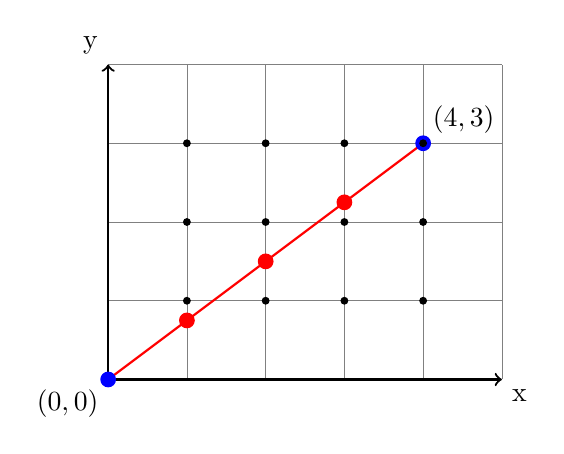
\begin{tikzpicture}[scale=1]
        \draw[step=1cm,gray,very thin] (0,0) grid (5,4);
    
        \draw[thick,->] (0,0) -- (5,0) node[anchor=north west] {x};
        \draw[thick,->] (0,0) -- (0,4) node[anchor=south east] {y};
    
        \draw[thick,red] (0,0) -- (4,3);
    
        \fill[blue] (0,0) circle (0.1);
        \node[below left] at (0,0) {$(0,0)$};
        \fill[blue] (4,3) circle (0.1);
        \node[above right] at (4,3) {$(4,3)$};
    
        \foreach \x in {1,2,3,4} {
            \foreach \y in {1,2,3} {
                \fill[black] (\x,\y) circle (0.05);
            }
        }
    
        \fill[red] (1,0.75) circle (0.1); % (1,0.75)
        \fill[red] (2,1.5) circle (0.1);  % (2,1.5)
        \fill[red] (3,2.25) circle (0.1); % (3,2.25)
    \end{tikzpicture}
\end{center}

\vspace{0.5cm}

次に、$(x, y)$が互いに素ではない場合、つまり最大公約数が1よりも大きい場合を考えます。このとき、$x = g \cdot x', y = g \cdot y'$と表すことができます。$g$が1よりも大きい場合は、
$(0, 0)$と$(x, y)$を結ぶ線分は格子点を通ることがあります。この$(x, y)$を最大公約数$g = 4$で割ると、$(0, 0)$と$(3, 1)$となり、3と1は互いに素です。先ほどのように互いに素の場合は
格子点は存在しません。$d = 4$というのはこの互いに素という格子点の最小単位が4つであることを示しています。今回の設定では、線分の端は格子点に含まれないので、格子点の個数は$4 - 1 = 3$個です。

\vspace{0.5cm}

\begin{center}
    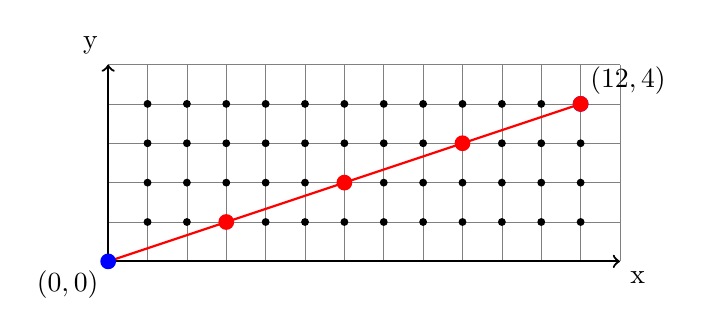
\begin{tikzpicture}[scale=0.5]
        % Draw the grid
        \draw[step=1cm,gray,very thin] (0,0) grid (13,5);
    
        % Draw the x and y axes
        \draw[thick,->] (0,0) -- (13,0) node[anchor=north west] {x};
        \draw[thick,->] (0,0) -- (0,5) node[anchor=south east] {y};
    
        % Draw the line segment from (0,0) to (12,4)
        \draw[thick,red] (0,0) -- (12,4);
    
        % Mark the points (0,0) and (12,4)
        \fill[blue] (0,0) circle (0.2);
        \node[below left] at (0,0) {$(0,0)$};
        \fill[blue] (12,4) circle (0.2);
        \node[above right] at (12,4) {$(12,4)$};
    
        % Mark the grid points around the line segment
        \foreach \x in {1,...,12} {
            \foreach \y in {1,...,4} {
                \fill[black] (\x,\y) circle (0.1);
            }
        }
    
        % Highlight the points that lie on the line segment
        \foreach \i in {3,6,9,12} {
            \fill[red] (\i,{\i/3}) circle (0.2);
        }
    
    \end{tikzpicture}
\end{center}

\vspace{0.5cm}

実装例を以下に示します。

\begin{lstlisting}[caption=2点間の格子点の個数の実装, label=grid, frame=TRBL]
def GCD(a: int, b: int) -> int:
    if a < b:
        a, b = b, a
    if b == 0:
        return a
    
    return GCD(b, a % b)

def count_grid_points(x1: int, y1: int, x2: int, y2: int) -> int:
    x, y = abs(x1 - x2), abs(y1 - y2)
    return GCD(x,y) - 1
\end{lstlisting}

他にも様々な性質があります。

\begin{theorembox}[互いに素と一次不定方程式]
    $a, b \in \mathbb{Z}$が互いに素であるとき、
    \begin{equation*}
        ax + by = 1
    \end{equation*}
    を満たす$x, y \in \mathbb{Z}$が存在する。
\end{theorembox}

これは上で見た拡張ユークリッドの互除法そのものです。

\begin{theorembox}
    $a, b \in \mathbb{Z}$が互いに素であるとき、$b \in \mathbb{Z}$に関して$bc$が$a$で割り切れるなら、
    $c$は$a$の倍数である。

    \textbf{証明}  \\
    $a, b$は互いに素であるから、$ax + by = 1$を満たす$x, y \in \mathbb{Z}$が存在する。
    \begin{equation*}
        c = c \times 1 = c (ax + by) = acx + bcy
    \end{equation*}
    $acx$は自明に$a$で割り切れる。$bcy$も条件より$a$で割り切れるから、$c$は$a$の倍数である。

\end{theorembox}

\begin{theorembox}[合同式の割り算]
    $a, m \in \mathbb{Z}$が互いに素であるとする。
    \begin{equation*}
        ax \equiv by \mod{m}
    \end{equation*}
    であるとき、
    \begin{equation*}
        x\equiv y (\mod{m})
    \end{equation*}
    が成立する。
\end{theorembox}

\begin{theorembox}[倍数の周期性]
    $a, m \in \mathbb{Z}$が互いに素であるとする。
    \begin{equation*}
        0, a, 2a, \cdots, (m - 1)a
    \end{equation*}
    を$m$で割った余りを昇順に並び替えると、$0, 1, 2, \cdots, m - 1$になる。
\end{theorembox}

\begin{theorembox}[逆元と合同方程式]
    $a, m \in \mathbb{Z}$が互いに素であるとする。任意の$b \in \mathbb{Z}$に対して、
    \begin{equation*}
        a x \equiv b \mod{m}
    \end{equation*}
    を満たす$x \in \mathbb{Z}$が$m$を法としてただ一つ在する。特に、$b = 1$の場合を逆元という。
\end{theorembox}

\newpage
\begin{tcolorbox}[enhanced,
    colback=white!85!gray,
    drop fuzzy shadow,
    boxrule=0.3mm,
    arc=0mm,
    left=0pt,
    top=0pt,
    sharp corners,
    width=\textwidth,
    ]
    \textbf{オイラー関数} \\
    オイラー関数とは、自然数$N$が与えられたときに、$1, 2, \cdots, N$のうち$n$と互いに素になる数の個数を求める関数$\Phi(N)$
    です。
  \tcblower
  
  \begin{tcolorbox}[
    coltext=white!10!blue,
    colback=white!90!purple!90!blue,
    drop fuzzy shadow,
    boxrule=0mm,
    arc=0mm,
    width=1.3cm,
    left=0pt,
    right=0pt,
    top=0pt,
    bottom=0pt,
    halign=flush left,
  ]
  \end{tcolorbox}
  \tcblower
  \textbf{回答:}
  \begin{lstlisting}
def enumerate_divisors(n: int) -> list[int]:
    divisors = set()
    for i in range(1, int(n ** 0.5) + 1):
        if n % i == 0:
            divisors.add(i)
            if i != n // i:
                divisors.add(n // i)
    
    return list(divisors)


def main():
    n = int(input())
    divisors = enumerate_divisors(n)
    
    print(*divisors)
    
if __name__ == "__main__":
    main()

  \end{lstlisting}
  \end{tcolorbox}% タイトルの独立

\subsection{問題}

問題1  yukicoder No.442 和と積 \\
2つの整数$a, b$が与えられるので、$a + b, a \times b$の最大公約数を求める問題です。
\begin{lstlisting}[caption=2点間の格子点の個数の実装, label=grid, frame=TRBL]
\end{lstlisting}

\textbf{参考}

\begin{itemize}
    \item \url{https://qiita.com/drken/items/ae02240cd1f8edfc86fd}
\end{itemize}

\section{冪乗: 繰り返し二乗法}

$x^n$を求める際に単に$x \times x \times \cdots \times x$と計算すると$O(n)$の計算量がかかります。繰り返し二乗法を用いると、$O(\log n)$で計算することができます。
また、冪乗では計算結果が非常に大きくなることがあるので、計算結果をmodで割った余りを求めることがあります。剰余で答えを出すときの演算によって処理が異なるので
注意が必要です。

\begin{itemize}
    \item 加算: 加算した後でmodを取る
    \item 減算: 減算した後でmodを取る
    \item 乗算: 乗算した後でmodを取る
    \item 除算: 計算途中でmodを取るときは逆元を用いる(後述)
\end{itemize}

\begin{lstlisting}[caption=繰り返し二乗法の実装, label=power, frame=TRBL]
def exp_mod(n: int, m: int, mod: int) -> int:
    if m == 0:
        return 1
    if m == 1:
        return n % mod
    ans = 1
    m1, m2 = m // 2, m % 2
    ans *= exp_mod(n, m1, mod) % mod
    ans = (ans * ans) % mod
    
    ans *= exp_mod(n, m2, mod)
    ans %= mod
    
    return ans
\end{lstlisting}

\section{逆元とフェルマーの小定理}

% 乗算のmodは計算結果と計算途中でmodを取ると結果が違いことを説明する
除算のmodを取るとき、計算途中でmodをもとった場合と最後にmodを取った場合で結果が異なることがあります。例えば、$a = 20, b = 4, mod = 6$で考えます。

\begin{itemize}
    \item \textbf{計算途中でmodを取る場合:}
    \begin{enumerate}
        \item まず、\( a \) と \( b \) に対してmodを取ります:
        \[
        a \mod m = 20 \mod 6 = 2
        \]
        \[
        b \mod m = 4 \mod 6 = 4
        \]
        \item 次に、得られたmodの値で除算を行い、さらにmodを取ります:
        \[
        \left(\frac{a \mod m}{b \mod m}\right) \mod m = \left(\frac{2}{4}\right) \mod 6
        \]
        通常の整数除算では、これは0(小数は考慮しない)となるため、
        \[
        0 \mod 6 = 0
        \]
        結果は \( 0 \) になります。
    \end{enumerate}

    \item \textbf{最後にmodを取る場合:}
    \begin{enumerate}
        \item まず、\( a \) を \( b \) で割ります:
        \[
        \frac{20}{4} = 5
        \]
        \item 次に、その結果に対してmodを取ります:
        \[
        5 \mod 6 = 5
        \]
    \end{enumerate}
\end{itemize}

除算のmodを求めるときは、計算途中でmodを取ると結果が異なることがあるので、逆元を用いて計算します。

\subsection{フェルマーの小定理と逆元}

除算におけるmodを考えるために\textbf{フェルマーの小定理}と\textbf{逆元}を導入します。

\begin{tcolorbox}[enhanced,title=フェルマーの小定理, 
    attach boxed title to top left, 
    colback=white!95!blue,
    colbacktitle=white!10!blue!50!black,
    drop fuzzy shadow,
    boxrule=0.25mm,
    ]
    $a$は任意の自然数、$m$を素数で$a, m$が互いに素であるとき、以下の式が成り立つ。
    \begin{equation*}
        a^{m-1} \equiv 1 \pmod{m}
    \end{equation*}
  \end{tcolorbox}

\begin{tcolorbox}[enhanced,title=逆元, 
    attach boxed title to top left, 
    colback=white!95!blue,
    colbacktitle=white!10!blue!50!black,
    drop fuzzy shadow,
    boxrule=0.25mm,
    ]
    $m$が素数で、$a$が$m$では割り切れない整数であるとき、以下の式を満たす$x$が[1, m)の範囲で一意に存在する。
    このような$x$を $\pmod m$における$a$の逆元と呼ぶ。
    \begin{equation*}
        a x \equiv 1 \pmod{m}
    \end{equation*}
  \end{tcolorbox}
  ここで、$a^{m-1} \equiv a \times a^{m-2} \equiv 1 \pmod{m}$となるので、$a^{m-2}$が$a$の逆元であることがわかります。以上より以下のことがわかります。

  \vspace{0.5cm}

  \begin{center}
    \textbf{aで割ることは、aの逆元をかけることと等しい}
  \end{center}

\subsection{問題}
逆元を使った問題を解いてみましょう。

  \begin{tcolorbox}[enhanced,
    colback=white!85!gray,
    drop fuzzy shadow,
    boxrule=0.3mm,
    arc=0mm,
    left=0pt,
    top=0pt,
    sharp corners,
    width=\textwidth,
    ]
    \textbf{問題}
    ${}_n \mathrm{C}_k$を998244353で割ったあまりを求めるプログラムを作成せよ。
  \tcblower

  \begin{tcolorbox}[
    coltext=white!10!blue,
    colback=white!90!purple!90!blue,
    drop fuzzy shadow,
    boxrule=0mm,
    arc=0mm,
    width=1.3cm,
    left=0pt,
    right=0pt,
    top=0pt,
    bottom=0pt,
    halign=flush left,
  ]
  \end{tcolorbox}
  \tcblower
  \textbf{回答} 
  ${}_n \mathrm{C}_k = \frac{n!}{(n - k)! k!}$の剰余を求めるます。$\mod$の世界で除算が登場しているので、逆元を用いて計算します。
  乗算するのは$(n - k)!, k!$であることから、これらで割ることは$\mod$の世界では、これらの逆元つまり、それぞれ$(n - k)!^{(DIV-2)}, k!^{(DIV-2)}$をかけることと等しいです。
  \begin{lstlisting}[caption=${}_n \mathrm{C}_k$を求める, label=combination]
DIV = 998244353

def factorial(n: int) -> list[int]:
    memo = [1] * (n + 1)
    for i in range(1, n + 1):
        memo[i] = (memo[i-1] * i) % DIV
    
    return memo

def inverse(n: int) -> int:
    return pow(n, DIV - 2, DIV)

def comb(n: int, k: int, memo: list[int]) -> int:
    return (memo[n] * inverse(memo[k]) * inverse(memo[n-k])) % DIV
 
n, k = map(int, input().split())
memo = factorial(n)
print(comb(n, k, memo) % DIV)
  \end{lstlisting}
  \end{tcolorbox}% 

EEIC2024アルゴリズムの授業で扱ったデータ構造のアルゴリズムのシケプリです。扱った内容は以下の通りです。
\begin{itemize}
	\item スタック
	\item キュー
	\item 線形リスト
	\item ツリー
	\item ヒープ
	\item セグメント木(発展的な内容)
	\item BIT(発展的な内容)
\end{itemize}

\section{スタック}

スタックはLIFO(Last In First Out)といって、最後に入れたデータが最初に取り出されるデータ構造です。本を積み重ねるイメージで考えるとわかりやすいです。スタックには以下の操作があります。

\begin{itemize}
	\item push: スタックにデータを追加する
	\item pop: スタックからデータを取り出す
\end{itemize}

\vspace{1cm}

\begin{center}
\begin{tikzpicture}
		\draw (0, 0) rectangle (1, 1);
		\node at (0.5, 0.5) {8};
		\draw (0, 1) rectangle (1, 2);
		\node at (0.5, 1.5) {4};
		\draw (0, 2) rectangle (1, 3);
		\node at (0.5, 2.5) {5};
		\draw (0, 3) rectangle (1, 4);
		\draw (0, 4) rectangle (1, 5);
	
		\draw (4, 0) rectangle (5, 1);
		\node at (4.5, 0.5) {8};
		\draw (4, 1) rectangle (5, 2);
		\node at (4.5, 1.5) {4};
		\draw (4, 2) rectangle (5, 3);
		\node at (4.5, 2.5) {5};
		\draw (4, 3) rectangle (5, 4);
		\node at (4.5, 3.5) {6};
		\draw (4, 4) rectangle (5, 5);
	
		\draw (8, 0) rectangle (9, 1);
		\node at (8.5, 0.5) {8};
		\draw (8, 1) rectangle (9, 2);
		\node at (8.5, 1.5) {4};
		\draw (8, 2) rectangle (9, 3);
		\node at (8.5, 2.5) {5};
		\draw (8, 3) rectangle (9, 4);
		\draw (8, 4) rectangle (9, 5);

		% pushと文字を描画
		\draw[->, very thick] (1.2, 3.5) -- (3.8, 3.5);
		\node at (2.5, 3.8) {push(6)};	

		% popと文字を描画
		\draw[->, very thick] (5.2, 3.5) -- (7.8, 3.5);
		\node at (6.5, 3.8) {pop()};
\end{tikzpicture}
\end{center}

\vspace{0.5cm}
\begin{center}
	\textbf{スタックのイメージ}
\end{center}
\vspace{0.5cm}

\subsection{スタックの実装}
実装のポイントは以下の3つです。Pythonのclassを使って実装します。
\begin{itemize}
	\item スタックは配列で実装する
	\item 要素が入る位置を示すポインタを持つ
	\item pushとpopのメソッドを実装する
\end{itemize}

実装は以下の\ref{stack}のようになります。

\begin{lstlisting}[caption=スタックの実装, label=stack, frame=TRBL, label={stack}]
	class Stack:
    def __init__(self, size: int) -> None:
        self.stack: list[int] = [0] * size
        self.top: int = 0
    
    def push(self, value: int) -> None:
        if self.top < len(self.stack):
            self.stack[self.top] = value
            self.top += 1
        else:
            print("This stack is full.")
    
    def pop(self) -> None:
        if self.top > 0:
            self.top -= 1
            return_value = self.stack[self.top]
            return return_value
        else:
            print("This stack is empty.")

def main():
    size = 5
    stack = Stack(size)
    
    stack.push(8)
    stack.push(4)
    stack.push(5)
    stack.push(6)
    return_value = stack.pop()
    
    print(f"returned value is {return_value}")
    
main()

\end{lstlisting}

\begin{tcolorbox}[enhanced, title=Column1 collections.deque, breakable, colback=white, drop fuzzy shadow, attach boxed title to top center={yshift*=0.1cm}]
	実際にスタックを使用するときは、Pythonの標準ライブラリであるcollectionsのdequeを使うと便利です。PythonではStack スタックやキューが明示的に用意されていないため、双方向キューであるdequeを使ってスタックやキューを使用します。
	スタックは上記のように配列で簡単に実装可能ですが、標準ライブラリのdequeを使うことで、より高速にスタックを使用できます。

	\begin{lstlisting}[caption=スタックの実装, label=stack, frame=TRBL]
		def main():
    from collections import deque
    stack = deque()
    
    stack.append(8)
    stack.append(4)
    stack.append(5)
    stack.append(6)
    
    return_value = stack.pop()
    
    print(f"returned value is {return_value}")
    
main()
    	
	\end{lstlisting}
\end{tcolorbox}

\newpage

\section{キュー}
キューはFIFO(First In First Out)といって、最初に入れたデータが最初に取り出されるデータ構造です。ディズニーランドの待ち行列のようなイメージで考えるとわかりやすいです。
キューには以下のような操作があります。

\begin{itemize}
	\item enqueue: キューにデータを追加する
	\item dequeue: キューからデータを取り出す
\end{itemize}

先ほどのスタックと違って配列の頭からデータを取り出していることに注意してください。つまり、dequeueをするたびに
取り出すデータの位置をずらす必要があります。従って、データを取り出すための先頭アドレス、データを追加するための末尾アドレスを持つ必要があります。

しかし、ここで困ったことがあります。dequeueをするたびに配列の頭が右にずれていくと、配列の先頭にデータが残っているにも関わらず、配列の末尾にデータが追加できなくなります。この問題を解決するために、リングバッファ
というデータ構造を使います。

\vspace{1cm}

\begin{center}
	\begin{tikzpicture}
		\draw (0, 0) rectangle (1, 1);
		\node at (0.5, 0.5) {8};
		\draw (1, 0) rectangle (2, 1);
		\node at (1.5, 0.5) {4};
		\draw (2, 0) rectangle (3, 1);
		\node at (2.5, 0.5) {5};
		\draw (3, 0) rectangle (4, 1);
		\draw (4, 0) rectangle (5, 1);

		% enqueueの丸と矢印を描画
		\draw (6.5, 0.5) circle[radius=0.5];
		\draw [<-] (5.2, 0.5) -- (6.0, 0.5);
		\node at (6.5, 0.5) {2};

		\draw (0, -3) rectangle (1, -2);
		\node at (0.5, -2.5) {8};
		\draw (1, -3) rectangle (2, -2);
		\node at (1.5, -2.5) {4};
		\draw (2, -3) rectangle (3, -2);
		\node at (2.5, -2.5) {5};
		\draw (3, -3) rectangle (4, -2);
		\node at (3.5, -2.5) {2};
		\draw (4, -3) rectangle (5, -2);

		% dequeueの丸と矢印を描画
		\draw (-1.0, -2.5) circle[radius=0.5];
		\draw [<-] (-2.5, -2.5) -- (-1.5, -2.5);
		\node at (-1.0, -2.5) {8};

		\draw (0, -6) rectangle (1, -5);
		\draw (1, -6) rectangle (2, -5);
		\node at (1.5, -5.5) {4};
		\draw (2, -6) rectangle (3, -5);
		\node at (2.5, -5.5) {5};	
		\draw (3, -6) rectangle (4, -5);
		\node at (3.5, -5.5) {2};
		\draw (4, -6) rectangle (5, -5);

		% enqueueと文字を描画
		\draw[->, very thick] (2.4, -1.0) -- (2.4, -1.8);
		\node at (2.5, -0.8) {enqueue(2)};

		% dequeueと文字を描画
		\draw[->, very thick] (2.4, -4.0) -- (2.4, -4.8);
		\node at (2.5, -3.8) {dequeue()};

	
	\end{tikzpicture}
\end{center}

\begin{adjustbox}{center}
	% 初期状態:3要素が入っている状態
	\begin{tikzpicture}
		\draw (0, 0) circle[radius=2];
		\draw (0, 0) circle[radius=1.5];
	
		\foreach \i in {0, 1, 2, 3, 4, 5, 6, 7} {
			\node at ({360/8 * \i}:2.2) {\i};
		}
	
		\foreach \i in {0, 1,  7} {
			\draw[fill=blue!30] ({360/8 * \i}:1.75) circle[radius=0.15];
		}
	
		\draw[->, thick] (-45:3.0) node[right]{head} -- (-45:2.5);
		\draw[->, thick] (90:3.0) node[above]{tail} -- (90:2.5);
	\end{tikzpicture}
	
	% 1要素追加:headが進む
	\begin{tikzpicture}
		\draw (0, 0) circle[radius=2];
		\draw (0, 0) circle[radius=1.5];
	
		\foreach \i in {0, 1, 2, 3, 4, 5, 6, 7} {
			\node at ({360/8 * \i}:2.2) {\i};
		}
	
		\foreach \i in {0, 1, 2, 7} {
			\draw[fill=blue!30] ({360/8 * \i}:1.75) circle[radius=0.15];
		}
	
		\draw[->, thick] (-45:3.0) node[right]{head} -- (-45:2.5);
		\draw[->, thick] (135:3.0) node[above]{tail} -- (135:2.5);
	\end{tikzpicture}

	
	% さらに1要素追加:headが進む
	\begin{tikzpicture}
		\draw (0, 0) circle[radius=2];
		\draw (0, 0) circle[radius=1.5];
	
		\foreach \i in {0, 1, 2, 5, 6} {
			\node at ({360/8 * \i}:2.2) {\i};
		}
	
		\foreach \i in {0, 1, 2} {
			\draw[fill=blue!30] ({360/8 * \i}:1.75) circle[radius=0.15];
		}
	
		\draw[->, thick] (0:3.0) node[right]{head} -- (0:2.5);
		\draw[->, thick] (135:3.0) node[above]{tail} -- (135:2.5);
	\end{tikzpicture}
	\end{adjustbox}

\vspace{0.5cm}

\hspace{6cm} \textbf{enqueue()}
\hspace{3cm} \textbf{dequeue()}

リングバッファの仕組みを見てみましょう。enqueueをするときはtailの位置にデータを追加しtailを1だけ進めます。dequeueをするときはheadの位置のデータを取り出しheadを1だけ進めます。headとtailが同じ位置になったときは、キューが空になります。
実装の際は、要素の数で割った余りを使ってheadとtailの位置を管理します。

\subsection{キューの実装}
キューの実装のポイントは以下の3つです。
\begin{itemize}
	\item キューは配列で実装する
	\item 取り出す位置を示すポインタと追加する位置を示すポインタの2つを持つ
	\item リングバッファをモジュロ演算で実装する (\%を使う)
	\item enqueueとdequeueのメソッドを実装する
\end{itemize}

\begin{lstlisting}[caption=キューの実装, frame=TRBL, label={queue}]
	class Queue:
    def __init__(self, size: int) -> None:
        self.queue = [0] * size
        self.size = 0
        self.head = 0
        self.tail = 0
        
    def enqueue(self, value: int) -> None:
        if not self.is_full():
            self.size += 1
            self.queue[self.tail] = value
            self.tail = (self.tail + 1) % len(self.queue)
        else:
            print("queue is full")
    
    def dequeue(self) -> int:
        if not self.is_empty():
            self.size -= 1
            return_value = self.queue[self.head]
            self.head = (self.head + 1) % len(self.queue)
            print(return_value)
        else:
            print("queue is empty")
        
    
    def is_empty(self):
        return self.size == 0

    def is_full(self):
        return self.size == len(self.queue)

queue = Queue(5)

queue.enqueue(8)
queue.enqueue(4)
queue.enqueue(5)

queue.enqueue(2)

queue.dequeue()

\end{lstlisting}

\begin{tcolorbox}[enhanced, title=Column2 collections.deque, breakable, colback=white, drop fuzzy shadow, attach boxed title to top center={yshift*=0.1cm}]
	スタックと同様にキューも実際に使用するときは、Pythonの標準ライブラリであるcollectionsのdequeを使うと便利です。
	
	\begin{lstlisting}[frame=TRBL]
		from collections import deque

queue = deque()

queue.append(8)
queue.append(4)
queue.append(5)

queue.append(2)

return_value = queue.popleft()

print(f"returned value is {return_value}")
	\end{lstlisting}
\end{tcolorbox}

\newpage

\section{線形リスト}

線形リストとは、以下の図のようにデータと次のポインタを持つデータを連結させるデータ構造です。
線形リストは必要なときに必要なデータを追加していくことができるため、空間計算量的に効率がいいです。しかし、データを取り出すときは
先頭から順番にたどる必要があるため、時間計算量的には効率が悪いです。

今回実装する線形リストは以下の操作ができるものです。

\begin{itemize}
	\item 片方向の線形リスト
	\item 新しい要素は常に末尾に追加する
	\item 検索は先頭から順番に行う
\end{itemize}

双方向の線形リストや、データの追加や削除を任意の位置で行うものもありますが、今回は片方向の線形リストを実装します。

\vspace{1cm}

\begin{tikzpicture}[node distance=6cm,baseline=-0.5ex,  arrow/.style = {thick,-stealth}]
    \node(NodeName1){
        \begin{tcolorbox}[width=4cm]
		データ1
		\tcblower
		次へのポインタ
        \end{tcolorbox}
    };
	\node(NodeName2)[right of=NodeName1]{
		\begin{tcolorbox}[width=4cm]
		データ2
		\tcblower
		次へのポインタ
		\end{tcolorbox}
	};
	\node(NodeName3)[right of=NodeName2]{
		\begin{tcolorbox}[width=4cm]
		データ3
		\tcblower
		次へのポインタ
		\end{tcolorbox}
	};

	% 矢印を描画
	\draw[arrow] (NodeName1) -- (NodeName2);
	\draw[arrow] (NodeName2) -- (NodeName3);
\end{tikzpicture}

\vspace{1cm}

\subsection{線形リストの実装}
先ほどのスタックやキューは配列を使って実装しましたが、線形リストはポインタ(Pythonではクラスのインスタンス)を使って要素をつなげて実装します。

\begin{lstlisting}[caption=線形リストの実装, label=linear, frame=TRBL, label={linear}]
class Node:
    def __init__(self, value) -> None:
        self.value = value
        self.next: Node = None
        
class LinkedList:
    def __init__(self) -> None:
        self.head = Node(None)
    
    def append(self, value: int) -> None:
        current_cell = self.head
        while current_cell.next != None:
            current_cell = current_cell.next
        
        # 追加する数値を値にもつノード
        new_cell = Node(value)
        # 現在の最後のノードの次のノードに付け加える
        current_cell.next = new_cell
        
    def pop(self, value: int) -> Node | None:
        """
        valueと同じ数値を値に持つノードを取り除く
        """
        prev_cell = None
        current_cell = self.head
        
        while current_cell != None:
            if current_cell.value == value:
                # 取り出すため、付け替える
                prev_cell.next = current_cell.next
                return value
            else:
                prev_cell = current_cell
                current_cell = current_cell.next
        
        return None

linked_list = LinkedList()

linked_list.append(10)
linked_list.append(535)
linked_list.append(51)
linked_list.append(40)
linked_list.append(40)
linked_list.append(1)

return_value = linked_list.pop(51)

print(return_value)

\end{lstlisting}

\newpage

\section{ツリー(木構造)}
木をひっくり返して根っこを上にして書いた木のような離散構造をツリーと言います。ツリーは用語が重要なため、以下の用語を覚えておくと良いです。

\subsection{木構造の用語}

\subsubsection{根と葉}

一番上のノードを\textbf{根}、一番下のノード(より下に子ノードを持っていないノード)\textbf{葉}といいます。

\vspace{1cm}

\begin{center}
	\begin{tikzpicture}[scale=0.4]
		\node[circle, draw, minimum size=1.2cm] (A) at (0, 0) {};
		\node[circle, draw, minimum size=1.2cm] (B) at (-4, -5) {};
		\node[circle, draw, minimum size=1.2cm] (C) at (4, -5) {};
		\node[circle, draw, minimum size=1.2cm] (D) at (-9, -10) {};
		\node[circle, draw, minimum size=1.2cm] (E) at (-13, -10) {};
		\node[circle, draw, minimum size=1.2cm] (F) at (-2, -10) {};
		\node[circle, draw, minimum size=1.2cm] (G) at (-6, -10) {};
		\node[circle, draw, minimum size=1.2cm] (H) at (2, -10) {};
	
		\draw (A) -- (B);
		\draw (A) -- (C);
		\draw (B) -- (D);
		\draw (B) -- (E);
		\draw (B) -- (F);
		\draw (B) -- (G);
		\draw (C) -- (H);

		% 円の中に文字を入れる
		\node at (0, 0) {根};

		% 葉には葉と書く
		\node at (-9, -10) {葉};
		\node at (-13, -10) {葉};
		\node at (-2, -10) {葉};
		\node at (-6, -10) {葉};
		\node at (2, -10) {葉};
	\end{tikzpicture}
\end{center}


\subsubsection{深さと高さ}

あるノードから繋がっている葉までの自分を除いたノードの数のうち最大の個数を\textbf{高さ}といいます。 葉ノード自体の高さは0です。また、
根からあるノードまでの高さを\textbf{深さ}といいます。

\vspace{1cm}
\begin{center}
	\begin{tikzpicture}[scale=0.4]
		\node[circle, draw, minimum size=1.2cm] (A) at (0, 0) {};
		\node[circle, draw, minimum size=1.2cm] (B) at (-4, -5) {};
		\node[circle, draw, minimum size=1.2cm] (C) at (4, -5) {};
		\node[circle, draw, minimum size=1.2cm] (D) at (-8, -10) {};
		\node[circle, draw, minimum size=1.2cm] (E) at (-0.5, -10) {};
		\node[circle, draw, minimum size=1.2cm] (F) at (-12, -15) {};
	
		\draw (A) -- (B);
		\draw (A) -- (C);
		\draw (B) -- (D);
		\draw (B) -- (E);
		\draw (D) -- (F);

		% 円の中に数字を入れる
		\node at (0, 0) {1};
		\node at (-4, -5) {2};
		\node at (4, -5) {3};
		\node at (-8, -10) {4};
		\node at (-0.5, -10) {5};
		\node at (-12, -15) {6};	

	\end{tikzpicture}
	\end{center}

\subsubsection{二分木(binary tree)}
すべてのノードに関して、その子ノードの数が2以下である木を\textbf{二分木}といいます。二分木は以下のような特徴があります。上の木も
二分木になっています。

また、、完全二分木というものがあります。完全二分技は英語で表記するとfull binary treeとcomplete binary treeがあります。これらは独立した定義ですので、注意してください。
違いを整理すると以下のようになります。

\begin{itemize}
	\item full binary tree: すべてのノードが0個または2個の子ノードを持つ二分木
	\item complete binary tree: 根がある階層(level)を除いて、すべての階層で埋まりうるノードがすべて埋まっているかつ、最後の階層のノードは左から右に向かって埋まっている二分木
\end{itemize}

両者の違いは最初は分かりにくいです、以下の図を見て理解を深めてください。

\vspace{1cm}

\begin{figure}[htbp]
\begin{center}
	\begin{tabular}{cc}
		\begin{tikzpicture}[scale=0.4]
			\node[circle, draw, minimum size=1.2cm] (A) at (0, 0) {};
			\node[circle, draw, minimum size=1.2cm] (B) at (-4, -5) {};
			\node[circle, draw, minimum size=1.2cm] (C) at (4, -5) {};
			\node[circle, draw, minimum size=1.2cm] (D) at (8, -10) {};
			\node[circle, draw, minimum size=1.2cm] (E) at (0, -10) {};

			\draw (A) -- (B);
			\draw (A) -- (C);
			\draw (C) -- (D);
			\draw (C) -- (E);
		\end{tikzpicture}

		& 
		\begin{tikzpicture}[scale=0.4]
			\node[circle, draw, minimum size=1.2cm] (A) at (0, 0) {};
			\node[circle, draw, minimum size=1.2cm] (B) at (-4, -5) {};
			\node[circle, draw, minimum size=1.2cm] (C) at (-6, -10) {};
			\node[circle, draw, minimum size=1.2cm] (D) at (-2, -10) {};
			\node[circle, draw, minimum size=1.2cm] (H) at (-8, -15) {};

			\node[circle, draw, minimum size=1.2cm] (E) at (4, -5) {};
			\node[circle, draw, minimum size=1.2cm] (F) at (8, -10) {};
			\node[circle, draw, minimum size=1.2cm] (G) at (2, -10) {};

			\draw (A) -- (B);
			\draw (B) -- (C);
			\draw (B) -- (D);

			\draw (A) -- (E);
			\draw (E) -- (F);
			\draw (E) -- (G);
			\draw (C) -- (H);

		\end{tikzpicture}
	\end{tabular}
\end{center}
\end{figure}

\hspace{1.5cm} full binary treeの例 \hspace{4.5cm} complete binary treeの例

\newpage

\section{ヒープ}
木構造を使ったデータ構造にヒープがあります。ヒープは以下の特徴があります。

\begin{itemize}
	\item 親ノードは子ノードよりも大きい(または小さい)という性質を持つ
	\item 根ノードは常に最大(または最小)となる
\end{itemize}

ヒープは最大値や最小値を根に持つため、最大値や最小値を取り出すのが高速です。
さらに今回はヒープの中でさらに、complete binary treeになっている\textbf{二分ヒープ}というデータ構造を扱います。ヒープはcomplete binary tree
に対して、以下の操作を行います。

\begin{itemize}
	\item 要素の追加
	\item 要素の取り出し
\end{itemize}

要素の追加に関して、二分ヒープがcomplete binary treeになっているため、根がある階層(level)の一番右に要素を追加してきます。
追加時に、追加したノードから根までヒープの条件を満たすように再帰的にノードを交換していきます。以下は最小ヒープの例です。

\begin{figure}[htbp]
	\begin{center}
		\begin{tabular}{cc}
			\begin{tikzpicture}[scale=0.4]
				\node[circle, draw, minimum size=1.2cm] (A) at (0, 0) {};
				\node[circle, draw, minimum size=1.2cm] (B) at (-4, -5) {};
				\node[circle, draw, minimum size=1.2cm] (C) at (4, -5) {};
				\node[circle, draw, minimum size=1.2cm] (D) at (-8, -10) {};
	
				% 線を引く
				\draw (A) -- (B);
				\draw (A) -- (C);
				\draw (B) -- (D);

				% 値を入れる
				\node at (0, 0) {1};
				\node at (-4, -5) {3};
				\node at (4, -5) {4};
				\node at (-8, -10) {6};
			\end{tikzpicture}
			&
			\begin{tikzpicture}[scale=0.4]
				\node[circle, draw, minimum size=1.2cm] (A) at (0, 0) {};
				\node[circle, draw, minimum size=1.2cm] (B) at (-4, -5) {};
				\node[circle, draw, minimum size=1.2cm] (C) at (4, -5) {};
				\node[circle, draw, minimum size=1.2cm] (D) at (-8, -10) {};
				\node[circle, draw, minimum size=1.2cm] (E) at (-1, -10) {};
	
				% 線を引く
				\draw (A) --(B);
				\draw (A) -- (C);
				\draw (B) -- (D);
				\draw (B) -- (E);

				% 値を入れる
				\node at (0, 0) {1};
				\node at (-4, -5) {3};
				\node at (4, -5) {4};
				\node at (-8, -10) {6};
				\node at (-1, -10) {2};
			\end{tikzpicture}
		\end{tabular}
		\begin{tikzpicture}[overlay, scale=0.4]
			\draw[->, thick] (-16, 0) -- (-13, 0);
			\node at (-14.7, -1.8) {追加};
		\end{tikzpicture}
	\end{center}
	\end{figure}

2を追加すると、第二階層において親の値は子以下であるという性質を満たさなくなってしまいます。そこで、2と3を交換します。実装としては
追加したノードから根に向かって再帰的に親ノードと比較してヒープの条件を満たすまでノードを交換していきます。

\begin{center}
	\begin{tikzpicture}[scale=0.4]
		\node[circle, draw, minimum size=1.2cm] (A) at (0, 0) {};
		\node[circle, draw, minimum size=1.2cm] (B) at (-4, -5) {};
		\node[circle, draw, minimum size=1.2cm] (C) at (4, -5) {};
		\node[circle, draw, minimum size=1.2cm] (D) at (-8, -10) {};
		\node[circle, draw, minimum size=1.2cm] (E) at (-1, -10) {};

		% 線を引く
		\draw (A) --(B);
		\draw (A) -- (C);
		\draw (B) -- (D);
		\draw (B) -- (E);

		% 値を入れる
		\node at (0, 0) {1};
		\node at (-4, -5) {2};
		\node at (4, -5) {4};
		\node at (-8, -10) {6};
		\node at (-1, -10) {3};
	\end{tikzpicture}
\end{center}

\vspace{1cm}

二分ヒープからの削除は少し複雑です。ヒープでは必ず根から取り出すことに注意してください。以下のような操作を行います。

\begin{enumerate}
	\item 根ノードを取り除く
	\item 一番右下のノードを根に移動する
	\item 根から下に向かって、子ノードと比較して、ヒープの条件を満たすように再帰的にノードを交換していく
\end{enumerate}

一番右のノードを根に移動する理由は、complete binary treeを保つためです。もしも、根を取り除いた後に直接根の子ノード
を根にしてしまうと、必ずしもcomplete binary treeにならず実装が複雑になります。

\begin{figure}[htbp]
	\begin{center}
		\begin{tabular}{cc}
			\begin{tikzpicture}[scale=0.4]
				\node[circle, draw, minimum size=1.2cm] (A) at (0, 0) {};
				\node[circle, draw, minimum size=1.2cm] (B) at (-4, -5) {};
				\node[circle, draw, minimum size=1.2cm] (C) at (4, -5) {};
				\node[circle, draw, minimum size=1.2cm] (D) at (-8, -10) {};
				\node[circle, draw, minimum size=1.2cm] (E) at (-1, -10) {};
	
				% 線を引く
				\draw (A) -- (B);
				\draw (A) -- (C);
				\draw (B) -- (D);
				\draw (B) -- (E);

				% 値を入れる
				\node at (0, 0) {1};
				\node at (-4, -5) {3};
				\node at (4, -5) {4};
				\node at (-8, -10) {6};
				\node at (-1, -10) {2};
			\end{tikzpicture}
			&
			\begin{tikzpicture}[scale=0.4]
				\node[circle, draw, minimum size=1.2cm, dashed] (A) at (0, 0) {};
				\node[circle, draw, minimum size=1.2cm] (B) at (-4, -5) {};
				\node[circle, draw, minimum size=1.2cm] (C) at (4, -5) {};
				\node[circle, draw, minimum size=1.2cm] (D) at (-8, -10) {};
				\node[circle, draw, minimum size=1.2cm] (E) at (-1, -10) {};
	
				% 線を引く
				\draw (A) --(B);
				\draw (A) -- (C);
				\draw (B) -- (D);
				\draw (B) -- (E);

				% 値を入れる
				\node at (-4, -5) {3};	
				\node at (4, -5) {4};
				\node at (-8, -10) {6};
				\node at (-1, -10) {2};
				
			\end{tikzpicture}
		\end{tabular}
		\begin{tikzpicture}[overlay, scale=0.4]
			\draw[->, thick] (-16, 0) -- (-13, 0);
			\node at (-14.7, -1.8) {1.根を除く};
		\end{tikzpicture}
	\end{center}
	\end{figure}


\begin{figure}[htbp]
	\begin{center}
		\begin{tabular}{cc}
			\begin{tikzpicture}[scale=0.4]
				\node[circle, draw, minimum size=1.2cm, dashed] (A) at (0, 0) {};
				\node[circle, draw, minimum size=1.2cm] (B) at (-4, -5) {};
				\node[circle, draw, minimum size=1.2cm] (C) at (4, -5) {};
				\node[circle, draw, minimum size=1.2cm] (D) at (-8, -10) {};
				\node[circle, draw, minimum size=1.2cm] (E) at (-1, -10) {};
	
				% 線を引く
				\draw (A) -- (B);
				\draw (A) -- (C);
				\draw (B) -- (D);
				\draw (B) -- (E);

				% 値を入れる
				\node at (0, 0) {};
				\node at (-4, -5) {3};
				\node at (4, -5) {4};
				\node at (-8, -10) {6};
				\node at (-1, -10) {2};
			\end{tikzpicture}
			&
			\begin{tikzpicture}[scale=0.4]
				\node[circle, draw, minimum size=1.2cm] (A) at (0, 0) {};
				\node[circle, draw, minimum size=1.2cm] (B) at (-4, -5) {};
				\node[circle, draw, minimum size=1.2cm] (C) at (4, -5) {};
				\node[circle, draw, minimum size=1.2cm] (D) at (-8, -10) {};
	
				% 線を引く
				\draw (A) --(B);
				\draw (A) -- (C);
				\draw (B) -- (D);

				% 値を入れる
				\node at (0, 0) {2};
				\node at (-4, -5) {3};	
				\node at (4, -5) {4};
				\node at (-8, -10) {6};
				
			\end{tikzpicture}
		\end{tabular}
		\begin{tikzpicture}[overlay, scale=0.4]
			\draw[->, thick] (-16, 0) -- (-13, 0);
			\node at (-14.7, -1.8) {2.右下を根に};
		\end{tikzpicture}
	\end{center}
	\end{figure}

上の例では、根を取り除き一番右のノードを根に移動すると木がヒープの性質を満たしていますが、一般的にはヒープの性質を満たすまで
根から下に向かってノードを再帰的に交換していきます。

二分ヒープの実装のポイントは

\begin{itemize}
	\item 1-indexedの配列で実装する(要素数 + 1の大きさの配列を用意する)
	\item 追加、削除時にヒープの条件を満たす様に再帰的に更新する
\end{itemize}


二分木は構造体を使わず配列だけで実装できる点が利点です。以下は最小ヒープの実装です。

\begin{lstlisting}[caption=二分ヒープの実装, label=binaryheap, frame=TRBL, label={binaryheap}]
class Heap:
	def __init__(self, size: int) -> None:
		self.inf = 1 << 60
		self.size = size + 1
		self.heap = [self.inf] * self.size
		self.tail = 0 # 現在のヒープのデータ数
		
	def swap(self, index1: int, index2: int) -> None:
		self.heap[index1], self.heap[index2] = self.heap[index2], self.heap[index1]

	def push(self, value: int) -> None:
		if self.tail != self.size - 1:
			self.tail += 1
			self.heap[self.tail] = value
			self.check_from_leaf(self.tail)

	def check_from_leaf(self, node: int) -> None:
		# nodeが根なら再帰終了
		if node == 1:
			return
		
		parent = node // 2
		# ヒープの条件を満たさない
		if self.heap[parent] > self.heap[node]:
			self.swap(parent, node)
			self.check_from_leaf(parent)
		

	def pop(self) -> int | None:
		if self.tail != 0:
			popping_value = self.heap[1]
			# 一番右の葉ノードを根ノードに移動
			self.heap[1] = self.heap[self.tail]
			self.tail -= 1
			self.check_from_root(1)
			return popping_value
		else:
			return None

	def check_from_root(self, node: int) -> None:
		left_child, right_child = 2 * node, 2 * node + 1
		
		# left > rightよりこれだけで十分
		if left_child > self.tail:
			return
		
		# 2つの子ノードの大小で区別する
		smaller_node = larger_node = 0
		if self.heap[left_child] < self.heap[right_child]:
			smaller_node, larger_node = left_child, right_child
		else:
			smaller_node, larger_node = right_child, left_child
		
		# 親ノードと小さい方の子ノードを比較
		if self.heap[node] > self.heap[smaller_node]:
			self.swap(node, smaller_node)
			# 小さい方だけで十分
			self.check_from_root(smaller_node)

\end{lstlisting}

\subsection{問題}
問題1 \\
ABC 141 D - Powerful Discount Tickets \\
とにかく一番高い商品の値段を半分の値段で買っていくのが良さそうです。上で実装した自作ヒープと
Pythonの標準ライブラリのheapqの両方を使って解きます。

\begin{lstlisting}[caption=問題1, label=問題1: heap, frame=TRBL]
class MinHeap:
    def __init__(self, size: int) -> None:
        self.inf = 1 << 60
        self.size = size + 1
        self.heap = [self.inf] * self.size
        self.tail = 0
    
    def _swap(self, index1: int, index2: int) -> None:
        self.heap[index1], self.heap[index2] = self.heap[index2], self.heap[index1]
    
    def push(self, value: int) -> None:
        if self.size - 1 <= self.tail:
            raise OverflowError("the heap is full")
        
        self.tail += 1
        self.heap[self.tail] = value
        
        self._reflesh_from_leaf(self.tail)
    
    def _reflesh_from_leaf(self, node: int) -> None:
        if node == 1:
            return
        
        child = node
        parent = child // 2
        
        if self.heap[child] < self.heap[parent]:
            self._swap(child, parent)
            self._reflesh_from_leaf(parent)
    
    def pop(self) -> int | None:
        if self.tail == 0:
            return None

        popping_value = self.heap[1]
        self.heap[1] = self.heap[self.tail]
        self.heap[self.tail] = self.inf
        self.tail -= 1
        
        self._refresh_from_root(1)
        
        return popping_value

    def _refresh_from_root(self, node: int) -> None:
        if node > self.tail:
            return 
        left, right = 2 * node, 2 * node + 1
        
        if left <= self.tail and self.heap[node] > self.heap[left]:
            self._swap(node, left)
        
        if right <= self.tail and self.heap[node] > self.heap[right]:
            self._swap(node, right)
        
        self._refresh_from_root(left)
        self._refresh_from_root(right)
    
    def all(self) -> int:
        sm = 0
        for i in range(1, self.tail + 1):
            sm += self.heap[i]
        
        return sm
    
def main():
    n, m = map(int, input().split())
    A = list(map(int, input().split()))

    heap = MinHeap(len(A))
    
    for a in A:
        heap.push(-a)
    
    for _ in range(m):
        max_price = -heap.pop()
        discounted_price = max_price // 2
        
        heap.push(-discounted_price)
        
    print(-heap.all())
    
    
if __name__ == "__main__":
    main()


# 別解 heapqを使用
from heapq import heapify, heappush, heappop
    
def main():
    n, m = map(int, input().split())
    A = list(map(int, input().split()))
    
    # heapqは最小ヒープになっているため
    for i in range(n):
        A[i] = -A[i]
    
    heapify(A)
    
    for _ in range(m):
        max_price = -heappop(A)
        discount_price = max_price // 2
        heappush(A, -discount_price)
        
    print(- sum(A))

if __name__ == "__main__":
    main()

\end{lstlisting}


\newpage

\section{セグメント木}
セグメント木はある条件を満たす演算に関する区間の計算結果を高速に求めるデータ構造です。区間の計算結果を高速にもとめると聞いて
累積和や尺取法を思い浮かべるかもしれませんが、セグメント木は扱うデータの要素が逐一変わるような状況でも区間の計算結果を高速に求めることができます。
具体的な演算は、区間の最大・最小値や、合計値などがあります。

\subsection{数学の知識の確認}
セグメント木の内容に入る前に、セグメント木を理解するのに必要な数学の知識を整理します。

\subsubsection{二項演算}

自然数や文字列の集合$S$の任意2つの元から新たに値を生成する操作のことを\textbf{$S$上の二項演算}といいます。
特に、$x, y \in S$に対する二項演算を$op(x, y)$と書き、

% equation*とすると、数式の番号がつかなくなる. 
\begin{equation*}
	op(x, y) = x * y
\end{equation*}

と表現することにします。

\subsubsection{閉じた演算}
$x, y \in S$に対して$op(x, y) \in S$を満たすような演算を閉じた演算といいます。例えば、自然数の集合$S$において、
$op(x, y) = x + y$は閉じた演算ですが、$op(x, y) = x - y$は閉じた演算ではありません。

今回実装するセグメント木は、閉じた演算を扱うため、セグメント木の演算は閉じた演算になるようにします。

\subsubsection{完全二分木}
セグメント木は完全二分木になっています。以下の図のように根以外のすべてのノードが2つの子ノードを持っていて、すべての葉の深さが同じ木になっています。

\vspace{0.25cm}

\begin{center}
\begin{tikzpicture}[scale=0.4]
    % ノードを描画
    \node[circle, draw, minimum size=1.2cm] (A) at (0, 0) {1};
    \node[circle, draw, minimum size=1.2cm] (B) at (-4, -5) {2};
    \node[circle, draw, minimum size=1.2cm] (C) at (4, -5) {3};
    \node[circle, draw, minimum size=1.2cm] (D) at (-6, -10) {4};
    \node[circle, draw, minimum size=1.2cm] (E) at (-2, -10) {5};
    \node[circle, draw, minimum size=1.2cm] (F) at (2, -10) {6};
    \node[circle, draw, minimum size=1.2cm] (G) at (6, -10) {7};

    % エッジを描画
    \draw (A) -- (B);
    \draw (A) -- (C);
    \draw (B) -- (D);
    \draw (B) -- (E);
    \draw (C) -- (F);
    \draw (C) -- (G);
\end{tikzpicture}
\end{center}

\subsection{セグメント木の仕組み}

セグメント木の理解に必要な知識の整理が終わったので、セグメント木の内容に入ります。

\subsubsection{セグメント木の構造}
セグメント木の構造の特徴は以下の通りです。下の図は$a_0からa_6$の7個のデータを持つセグメント木の例です。

\begin{itemize}
	\item 葉ノードにデータを持つ
	\item 親ノードは2つの子ノードの演算結果を持つ
	\item $op(x, y)$は結合法則を満たす ($(x * y) * z = x * (y * z)$が成立する)
	\item 集合$S$に対する$op$に単位元が存在する
\end{itemize}

\vspace{1cm}

\begin{center}
\begin{tikzpicture}[scale=0.7, transform shape]
    % ノードを描画
    \node[draw, rectangle, fill=cyan, minimum size=1.2cm] (A) at (0, 0) {?};
    \node[draw, rectangle, fill=cyan, minimum size=1.2cm] (B) at (-4, -3) {$(a_0 \star a_1) \star (a_2 \star a_3)$};
    \node[draw, rectangle, fill=cyan, minimum size=1.2cm] (C) at (4, -3) {?};
    \node[draw, rectangle, fill=cyan, minimum size=1.2cm] (D) at (-6, -6) {$a_0 \star a_1$};
    \node[draw, rectangle, fill=cyan, minimum size=1.2cm] (E) at (-2, -6) {$a_2 \star a_3$};
    \node[draw, rectangle, fill=cyan, minimum size=1.2cm] (F) at (2, -6) {$a_4 \star a_5$};
    \node[draw, rectangle, fill=cyan, minimum size=1.2cm] (G) at (6, -6) {?};
    \node[draw, rectangle, fill=cyan, minimum size=1.2cm] (H) at (-7, -9) {$a_0$};
    \node[draw, rectangle, fill=cyan, minimum size=1.2cm] (I) at (-5, -9) {$a_1$};
    \node[draw, rectangle, fill=cyan, minimum size=1.2cm] (J) at (-3, -9) {$a_2$};
    \node[draw, rectangle, fill=cyan, minimum size=1.2cm] (K) at (-1, -9) {$a_3$};
    \node[draw, rectangle, fill=cyan, minimum size=1.2cm] (L) at (1, -9) {$a_4$};
    \node[draw, rectangle, fill=cyan, minimum size=1.2cm] (M) at (3, -9) {$a_5$};
    \node[draw, rectangle, fill=cyan, minimum size=1.2cm] (N) at (5, -9) {$a_6$};
    \node[draw, rectangle, fill=cyan, minimum size=1.2cm] (O) at (7, -9) {?};

    % エッジを描画
    \draw (A) -- (B);
    \draw (A) -- (C);
    \draw (B) -- (D);
    \draw (B) -- (E);
    \draw (C) -- (F);
    \draw (C) -- (G);
    \draw (D) -- (H);
    \draw (D) -- (I);
    \draw (E) -- (J);
    \draw (E) -- (K);
    \draw (F) -- (L);
    \draw (F) -- (M);
    \draw (G) -- (N);
    \draw (G) -- (O);
\end{tikzpicture}
\end{center}

\vspace{1cm}

図には?があります。?を\textbf{全要素の総積をセグメント木の根が持つ}ように埋めていきます。下の図の$e$は単位元を表しています。
根$a_0 * a_1 * a_2 * a_3 * a_4 * a_5 * a_6$は全要素の総積になっていることを考えると、その下の?
は$a_4 * a_5 * a_6$になります。同様に、そのほかの?も埋めていくと以下の図のようになります。

\vspace{1cm}

\begin{center}
\begin{tikzpicture}[scale=0.7, transform shape]
    % ノードを描画
    \node[draw, rectangle, fill=cyan, minimum width=2.5cm, minimum height=1.2cm] (A) at (0, 0) {$a_0 \star a_1 \star a_2 \star a_3 \star a_4 \star a_5 \star a_6$};
    \node[draw, rectangle, fill=cyan, minimum width=2.5cm, minimum height=1.2cm] (B) at (-4, -3) {$a_0 \star a_1 \star a_2 \star a_3$};
    \node[draw, rectangle, fill=cyan, minimum width=2.5cm, minimum height=1.2cm] (C) at (4, -3) {$a_4 \star a_5 \star a_6$};
    \node[draw, rectangle, fill=cyan, minimum width=2.5cm, minimum height=1.2cm] (D) at (-6, -6) {$a_0 \star a_1$};
    \node[draw, rectangle, fill=cyan, minimum width=2.5cm, minimum height=1.2cm] (E) at (-2, -6) {$a_2 \star a_3$};
    \node[draw, rectangle, fill=cyan, minimum width=2.5cm, minimum height=1.2cm] (F) at (2, -6) {$a_4 \star a_5$};
    \node[draw, rectangle, fill=cyan, minimum width=2.5cm, minimum height=1.2cm] (G) at (6, -6) {$a_6$};
    \node[draw, rectangle, fill=cyan, minimum width=1.2cm, minimum height=1.2cm] (H) at (-7, -9) {$a_0$};
    \node[draw, rectangle, fill=cyan, minimum width=1.2cm, minimum height=1.2cm] (I) at (-5, -9) {$a_1$};
    \node[draw, rectangle, fill=cyan, minimum width=1.2cm, minimum height=1.2cm] (J) at (-3, -9) {$a_2$};
    \node[draw, rectangle, fill=cyan, minimum width=1.2cm, minimum height=1.2cm] (K) at (-1, -9) {$a_3$};
    \node[draw, rectangle, fill=cyan, minimum width=1.2cm, minimum height=1.2cm] (L) at (1, -9) {$a_4$};
    \node[draw, rectangle, fill=cyan, minimum width=1.2cm, minimum height=1.2cm] (M) at (3, -9) {$a_5$};
    \node[draw, rectangle, fill=cyan, minimum width=1.2cm, minimum height=1.2cm] (N) at (5, -9) {$a_6$};
    \node[draw, rectangle, fill=cyan, minimum width=1.2cm, minimum height=1.2cm] (O) at (7, -9) {$e$};

    % エッジを描画
    \draw (A) -- (B);
    \draw (A) -- (C);
    \draw (B) -- (D);
    \draw (B) -- (E);
    \draw (C) -- (F);
    \draw (C) -- (G);
    \draw (D) -- (H);
    \draw (D) -- (I);
    \draw (E) -- (J);
    \draw (E) -- (K);
    \draw (F) -- (L);
    \draw (F) -- (M);
    \draw (G) -- (N);
    \draw (G) -- (O);
\end{tikzpicture}
\end{center}

\vspace{1cm}

\subsection{セグメント木の実装}
セグメント木も二分木なので配列で表現することが可能です。ヒープと同様に1-indexedで実装します。以下の操作ができるようなセグメント木
を実装します。

\begin{itemize}
	\item セグメント木の構築
	\item 要素の更新
	\item 区間の演算結果の取得
\end{itemize}

\subsubsection{セグメント木の構築}
セグメント木では葉にデータが格納され、葉の数はデータの数以上でかつ$2^m$で表せられる最小の数になります。$2^m$は2進数表記にすると$2^m = 1\underbrace{00\cdots0}_{m}$となるので、2進数表記したときにm桁になる数と
$2^m$になる数であるときは葉の数を$2^m$にします。つまり、データの数$n$が$2^{m-1} + 1 \leq n \leq 2^m$であるとき、葉の数は$2^m$になります。そして今回のセグメント木は1-indexedのedの木になっているため配列の0番目の
要素は無視します。よって、配列全体の長さは$2 m$個になります。

セグメント木では扱う演算についての単位元を用意する必要があります。例えば、区間の最大値を求めるセグメント木では、単位元は$-\infty$になります。区間和では単位元は0になります。

葉をデータと単位元で埋めたら、その他のノードは2つの子ノードのデータを使って更新していきます。

\subsubsection{要素の更新}
更新クエリに対しては、該当する葉ノードを更新した後、その親ノードを更新していきます。

\subsubsection{区間の演算結果の取得}
区間の演算結果の取得は少々複雑です。何個か例を挙げて説明します。右開区間[left, right)の区間の演算結果を求めてみます。下のセグメント木を例にします。ノードの近くの数字は1-indexedな配列でセグメント木を表現し
したときのインデックス番号です。

・$left = 0, right = 3$のとき

求めるものは$a_0 * a_1 * a_2 = (a_0 * a_1) * a_1$つまり4と10の演算結果になります。 

・ $left = 1, right = 7$のとき

求めるものは$a_0 * a_1 * a_2 * a_3 * a_4 * a_5 * a_6 = a_1 * (a_2 * a_3) * (a_4 * a_5) * a_6$つまり、9と5と6と14の演算結果になります。

\vspace{1cm}

\begin{center}
	\begin{tikzpicture}[scale=0.7, transform shape]
		% ノードを描画
		\node[draw, rectangle, fill=cyan, minimum width=2.5cm, minimum height=1.2cm] (A) at (0, 0) {$a_0 \star a_1 \star a_2 \star a_3 \star a_4 \star a_5 \star a_6$};
		\node[draw, rectangle, fill=cyan, minimum width=2.5cm, minimum height=1.2cm] (B) at (-4, -3) {$a_0 \star a_1 \star a_2 \star a_3$};
		\node[draw, rectangle, fill=cyan, minimum width=2.5cm, minimum height=1.2cm] (C) at (4, -3) {$a_4 \star a_5 \star a_6$};
		\node[draw, rectangle, fill=cyan, minimum width=2.5cm, minimum height=1.2cm] (D) at (-6, -6) {$a_0 \star a_1$};
		\node[draw, rectangle, fill=cyan, minimum width=2.5cm, minimum height=1.2cm] (E) at (-2, -6) {$a_2 \star a_3$};
		\node[draw, rectangle, fill=cyan, minimum width=2.5cm, minimum height=1.2cm] (F) at (2, -6) {$a_4 \star a_5$};
		\node[draw, rectangle, fill=cyan, minimum width=2.5cm, minimum height=1.2cm] (G) at (6, -6) {$a_6$};
		\node[draw, rectangle, fill=cyan, minimum width=1.2cm, minimum height=1.2cm] (H) at (-7, -9) {$a_0$};
		\node[draw, rectangle, fill=cyan, minimum width=1.2cm, minimum height=1.2cm] (I) at (-5, -9) {$a_1$};
		\node[draw, rectangle, fill=cyan, minimum width=1.2cm, minimum height=1.2cm] (J) at (-3, -9) {$a_2$};
		\node[draw, rectangle, fill=cyan, minimum width=1.2cm, minimum height=1.2cm] (K) at (-1, -9) {$a_3$};
		\node[draw, rectangle, fill=cyan, minimum width=1.2cm, minimum height=1.2cm] (L) at (1, -9) {$a_4$};
		\node[draw, rectangle, fill=cyan, minimum width=1.2cm, minimum height=1.2cm] (M) at (3, -9) {$a_5$};
		\node[draw, rectangle, fill=cyan, minimum width=1.2cm, minimum height=1.2cm] (N) at (5, -9) {$a_6$};
		\node[draw, rectangle, fill=cyan, minimum width=1.2cm, minimum height=1.2cm] (O) at (7, -9) {$e$};
	
		% インデックス番号を追加
		\node at (0, 1) {1};
		\node at (-4, -2) {2};
		\node at (4, -2) {3};
		\node at (-6, -5) {4};
		\node at (-2, -5) {5};
		\node at (2, -5) {6};
		\node at (6, -5) {7};
		\node at (-7, -8) {8};
		\node at (-5, -8) {9};
		\node at (-3, -8) {10};
		\node at (-1, -8) {11};
		\node at (1, -8) {12};
		\node at (3, -8) {13};
		\node at (5, -8) {14};
		\node at (7, -8) {15};
	
		% エッジを描画
		\draw (A) -- (B);
		\draw (A) -- (C);
		\draw (B) -- (D);
		\draw (B) -- (E);
		\draw (C) -- (F);
		\draw (C) -- (G);
		\draw (D) -- (H);
		\draw (D) -- (I);
		\draw (E) -- (J);
		\draw (E) -- (K);
		\draw (F) -- (L);
		\draw (F) -- (M);
		\draw (G) -- (N);
		\draw (G) -- (O);
	\end{tikzpicture}
\end{center}

\vspace{1cm}

どのノードを使うかを機械的に判断していくにはどうすればいいでしょうか。それは、$left$と$right$が親ノードから見て右子ノードか左子ノードにあるかを見ていけばいいです。
leftとrightが右か左にあるかを見ていき、両者の間隔を狭めていって、leftとrightが同じノードになるまで続けます。

1. leftを右に移動する

leftが指すノードを使うか、それともその親ノードを使うかの判定を考えます。leftとrightの間は連続した区間であることに注意すると、leftが親の左側にある場合は親ノードの値を使えばいいことがわかります。
一方で、leftが親の右側にある場合は、leftが指すノードの値を使う必要があります。また1-indexedなセグメント木では右ノードと左ノードは偶奇で判定できます。

2. rightを左に移動する

rightも同様に考えます。ただ、rightは開区間になっているためright - 1を使うか使わないかを考えます。rightが親の左側にある時はright - 1よりも左側の要素を使うことになりますが、それはright - 1の親ノード
が含んでいるため、right - 1は使いません。一方、rightが親の右側にある場合はright - 1を使う必要があります。

\subsubsection{実装}

以上の考察をコードにします。以下は区間の最大値を求めるセグメント木の実装例です。


\begin{lstlisting}[caption=セグメント木の実装, label=segment, frame=TRBL, label={segment}]
# 区間の最大値を求めるセグメント木
class SegmentTree:
    def __init__(self, data_size: int, v: list[int] | None = None):
        self.data_size = data_size
        self.log = (data_size - 1).bit_length()
        self.capacity = 1 << self.log
        self.e = - (1 << 60)
        self.tree = [self.e] * (2 * self.capacity)

        # データが事前に与えられている場合
        if v is not None:
            # 葉ノードを埋める
            for i in range(self.data_size):
                 self.tree[self.capacity + i] = v[i]
                 
            # 葉ノード以外を埋める 
            for i in range(self.capacity - 1, 0, -1):
                self.update(i)
    
    def update(self, index: int) -> None:
        self.tree[index] = max(self.tree[2 * index], self.tree[2 * index + 1])

    # 更新クエリ
    def set(self, index: int, value: int) -> None:
        # 葉に移動
        index += self.capacity
        # 更新
        self.tree[index] = value
        # 上のノードを更新 根(1)を更新するまで続ける
        while index > 1:
            index //= 2
            self._update(index)
            
    # 取得クエリ
    def prod(self, left: int, right: int) -> int:
        left_value = right_value = self.e
        
        # 葉に移動
        left += self.capacity
        right += self.capacity
        
        while left < right:
            # 範囲の左側が右のノード、本実装では奇数
            if left % 2 == 1:
                left_value = max(left_value, self.tree[left])
                left += 1
            
            if right & 2 == 1:
                right -= 1
                right_value = max(right_value, self.tree[right])
                
            # 親に移動
            left //= 2 
            right //= 2
        
        return max(left_value, right_value)

    def all_prod(self):
        return self.tree[1]
    

\end{lstlisting}

\newpage

\section{BIT}
BIT(Binary Indexed Tree)はフェニック木とも呼ばれるデータ構造で、要素の値が変化する区間の\textbf{和}を高速に求めることができます。
セグメント木でも区間和の計算ができますが、BITはセグメント木よりもシンプルに実装が可能です。区間和に限定すればセグメント木は牛刀をもって鶏を割く
ようなものです。セグメント木はより一般的な演算に対応したデータ構造です。

BITはセグメント木に比べてシンプルです。

\subsection{和}

1番目からi番目の要素の和を高速に求めるために、以下のような操作を行います。

\begin{enumerate}
	\item iを2進数表記にしたときに一番右にある1の要素を足していく
	\item 1の要素を足していくときに、その要素を取り除いて次の1の要素を足していく
\end{enumerate}

例えば、$i = 7$の場合を考えると、$7 = 111(2)$となり、右から1を引いていくと、$111(2), 110(2), 100(2), 000(2)$、つまり$7, 6, 4, 0$となります。

BITのデータを持つ配列をbitとすると、1から7番目の要素の和は、bit[0] = 0になっているので、
\begin{equation*}
	\text{bit}[7] + \text{bit}[6] + \text{bit}[4] + \text{bit}[0]
\end{equation*}

になります。

\subsection{更新}

要素の更新は和の計算と逆の操作を行います。具体的には、以下の操作を行います。

\begin{enumerate}
	\item iを2進数表記にしたときに一番右にある1の要素を引いていく
	\item 1の要素を引いていくときに、その要素を取り除いて次の1の要素を引いていく
\end{enumerate}

例えば、$A = [1, 2, 3, 4, 5, 6, 7, 8]$という等差数列の5番目に6を足すと、$A = [1, 2, 3, 4, 11, 6, 7, 8]$になります。このような値の更新をBITで行ってみましょう。

まず、5を2進数で表すと、$101_2$となります。ここで、一番右にある1の桁に1を足す操作を順に行っていきます。$N = 8$を超える前に操作をやめます。

具体的には、$101_2 \rightarrow 110_2 \rightarrow 1000_2$ となります。これを10進数に直すと、5→6→8となります。ここで出てきた数をインデックスとして、6を足していくことで値を更新することができます。

実際の操作は以下のようになります。

\begin{verbatim}
BIT[5] += 6
BIT[6] += 6
BIT[8] += 6
\end{verbatim}

\subsection{実装}
BITの実装例は以下の通りです。

\begin{lstlisting}[caption=BITの実装, label=bit, frame=TRBL, label={bit}]
	class BIT:
    def __init__(self, size: int) -> None:
        self.size = size
        self.tree = [0] * (size + 1)
    
    def sum(self, index: int) -> int:
        res = 0
        while index > 0:
            res += self.tree[index]
            index -= index & (~index + 1)
        
        return res
    
    def update(self, index: int, value: int) -> None:
        while index < self.size:
            self.tree[index] += value
						index += index & (~index + 1)
\end{lstlisting}
\end{document}